% !TEX root = ../lectures_olympics.tex

\chapter{运动学}

自然界中的物体都处于从不间断的运动过程之中,真正绝对静止的物体其实是不存在的,所以我们学习物理的第一步自然就是要学会如何来描写各个物体的运动。
只有具备了相当数量刻画运动的方式,能够随心所欲地将任何物体的运动用科学的方法表示出来,才能够进一步研究物体运动状态的变化之间的联系,即物理学所想要告诉我们的自然界运行的基本规律。


\section{运动物体的抽象:质点}
和所有科学一样,物理的研究也是从最简单的对象开始,当把简单的问题研究清楚了以后逐渐地深入到更复杂的研究对象。
最简单的运动着的对象自然就是一个点,物理学中把一个运动着的点称之为一个{\heiti 质点}(mass point)。
用一个质点代表一个给定质量的点状物体的位置。
当然了,所有运动的对象实际上都有或简单或复杂的内部结构,但是如果它的形状和结构对于具体问题的研究影响不大时就可以将该对象看做一个几何上的点。


\begin{figure}[htbp]
\begin{center}
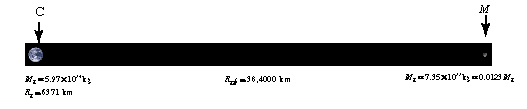
\includegraphics[width=0.9\textwidth]{images/motion-moon.pdf} 
\caption{月球和地球以及月地距离的真实尺寸}
\label{fig: 月球和地球以及月地距离的真实尺寸}
\end{center}
\end{figure}



能否将一个物体当做质点不仅与物体本身的大小有关,还与所研究的具体问题有关。
如果试图描写跳水运动员入水的动作时,他在入水过程中身体姿态至关重要,所以不能够当做质点来看待。
而在描写一个人从北京到上海的整个过程中,我们自然不必在意相对于上千公里的旅程中身体上各个部位之间的微小差别,这时一个人完全有理由当做一个质点。
同样如图\ref{fig: 月球和地球以及月地距离的真实尺寸}所示在研究月球围绕地球的转动时用一个点代表月球的位置相当精确,而在研究嫦娥号在月球上的着陆时月球肯定不能当做质点看待。



当把运动物体抽象为质点以后,它的位置就由这个点的空间位置来代表,这为我们描写运动带来了极大的简化,首先研究质点的运动,当掌握了足够的研究手段以后就有办法来描写真实物体的复杂运动了。
实际上,即使把运动物体简化为一个点它的运动也不是那么容易描写,为此我们将从最简单的运动形式出发,逐渐推广到一般的情况。
在掌握了描写质点或其它物理对象运动的方式以后将进一步研究支配它们运动背后的原因。


\section{最简单的运动:一维运动}




最简单的运动莫过于一个质点始终保持在一条直线上运动,就称它做直线运动。
一个做一维运动物体的位置的描写十分简单,只需要把一根{\heiti 数轴}(number line)放在它运动的直线上,选择任意一点当做数轴的原点,选择任意一个方向当做数轴的正方向,选择一个给定的长度当做计量长度的单位\footnote{物理学中通常选取米或千米来做为长度单位},一个质点的位置就可以用在该数轴上的坐标来唯一决定。
以这种方式选取的数轴称做描写该质点运动的{\heiti 坐标系(coordinate system)},而该质点某一时刻所在位置在坐标系中的读数就叫做它的{\heiti 位置(position)}或{\heiti 坐标}(coordinate)。
对于一维运动的质点,它在坐标系中的坐标通常用$x$来表示,不过这一点不是必须的。


一维运动的描写相对简单,只要知道了每一时刻它所处的位置就完全掌握了该质点的一维运动行为。
假设有一个质点,在时间$t=0\unit{s}$时的坐标为$x_0$,$t=1\unit{s}$时坐标为$x_1$,$t=2\unit{s}$时坐标为$x_2$……
当知道了它在很多时刻的坐标时,就在一定程度上掌握了它的运动行为,运动质点在不同时刻的坐标值知道的越多,我们对它的运动信息就知道地越多。
知道了一些坐标与时间的关系以后可以用很多方法把它的运动表现出来,以一个参加百米赛跑的运动员为例,描写他从起跑到终点的运动的方法有
\begin{description}
\item[叙述]  第1秒跑了1米,第2秒到了4米,第3秒到了9米,第4秒到了16米,第5秒末到了25米,第6秒末到了35米,第7秒末到了45米,第8秒到了55米,第9秒到了65米,第10秒到了75米,11秒85米,12秒100米,结束。
可以看出叙述的方法是能够为我们提供一些信息,但是有些繁琐,也不太直观。
这种描述方法在日常对话中比较常见,但对于科学研究却有些力不从心。
\item[列表] 同样的运动过程如果用一个表来表达,会节约很多空间。
对于同样的运动用列表法由\ref{tab: 不同时刻短跑选手的位置}给出
可以看到列表法会节省很多空间,但也有一些不够直观,无法快速得到运动快慢的信息。
实践上列表法更多地用于实验的数据的记录。
\begin{table}[htbp]
\begin{center}
\begin{tabular}{|c|c c c c c c c c c c c c|}
\hline
时间(s)&1&2&3&4&5&6&7&8&9&10&11&12\\
\hline
位置(m)&1&4&9&16&25&35&45&55&65&75&85&100\\
\hline

\end{tabular}
\caption{不同时刻短跑选手的位置}
\end{center}
\label{tab: 不同时刻短跑选手的位置}
\end{table}



\item[图像]
物理上最直观的描写质点运动的方法是图像法。
此时我们将建立一个坐标系,用横轴代表所经历的时间,纵轴则是已知时刻质点的位置。
对于前面的短跑选手,用图像法可以将他的运动用图\ref{fig: 短跑选手跑动距离和时间的图像}来描写。
从中可以看出,在比赛开始阶段他越跑越快,而随后一段时间里运动速度大致相同,最后在快接近终点的时候又有一个冲刺过程。
很明显可以看出,用图像来描写质点的运动具有最强的直观性。
\begin{figure}[htbp]
\begin{center}
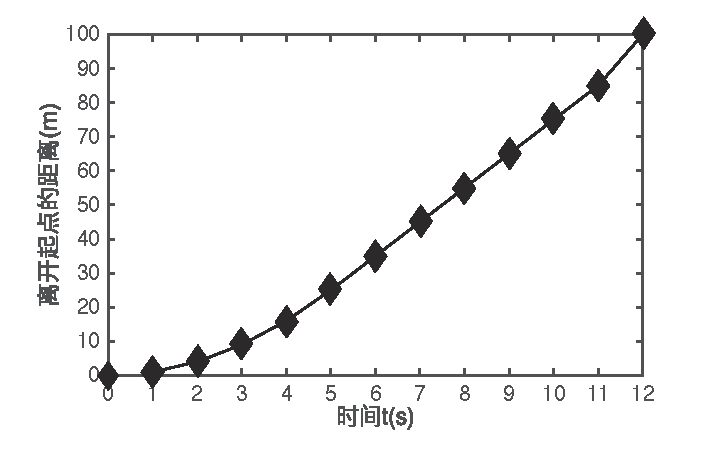
\includegraphics[width=0.5\textwidth]{images/motion-race.pdf}

\caption{短跑选手跑动距离和时间的图像}
\label{fig: 短跑选手跑动距离和时间的图像}
\end{center}
\end{figure}
\end{description}

不难发现以上的三种描写质点运动的方法都无法体现运动的一个最明显的特征:连续性。
运动的质点在每一时刻的位置一般来说都不相同,处于连续的变化过程当中。
为了体现这种特点,我们希望有一种办法对于每一个时刻都能够给出质点的位置,而不是仅仅给出几个特殊时刻的位置。
利用数学中的{\heiti 函数}可以帮助我们得到任意时刻运动质点的位置。
这时一个质点的运动可以表达为
\begin{equation}
x = x(t)
\end{equation}
当函数$x(t)$的形式为已知时,可以得到任意时刻质点所处的位置。
借助函数的图像可以形象地给出质点运动的特征。
例如当一个质点的运动可以用函数$x(t) = 3t$来描写,从中不但可以知道任意时刻质点的位置,还可以从函数的性质得知此时相同的时间里该质点会走过相同的距离。
假如另一个质点的运动函数为$x(t)=5t^2$,同样除了知道任意时刻的位置以及运动的其它性质。



\begin{example}
建立一个竖直向上的坐标系用来表示从它的原点处向上抛出物体的位置。
在不同的时间观察抛体的位置,某次实验得到的结果由下表给出,试着将测量值在坐标系中标出,并试着将其连接为一条光滑的曲线。

\begin{tabular}{|c|ccccccccccccc|}
\hline 
时间 & 0 & 0.5 & 1 & 1.5 & 2 & 2.5 & 3 & 3.5 & 4 & 4.5 & 5 & 5.5 & 6  \\ 
\hline 
位置 & 0 & 8.75 & 15 & 18.75 & 20 & 18.75 & 15 & 8.75 & 0 & -11.25 & -25 & -41.25 & -60 \\ 
\hline 
\end{tabular} 
\begin{center}
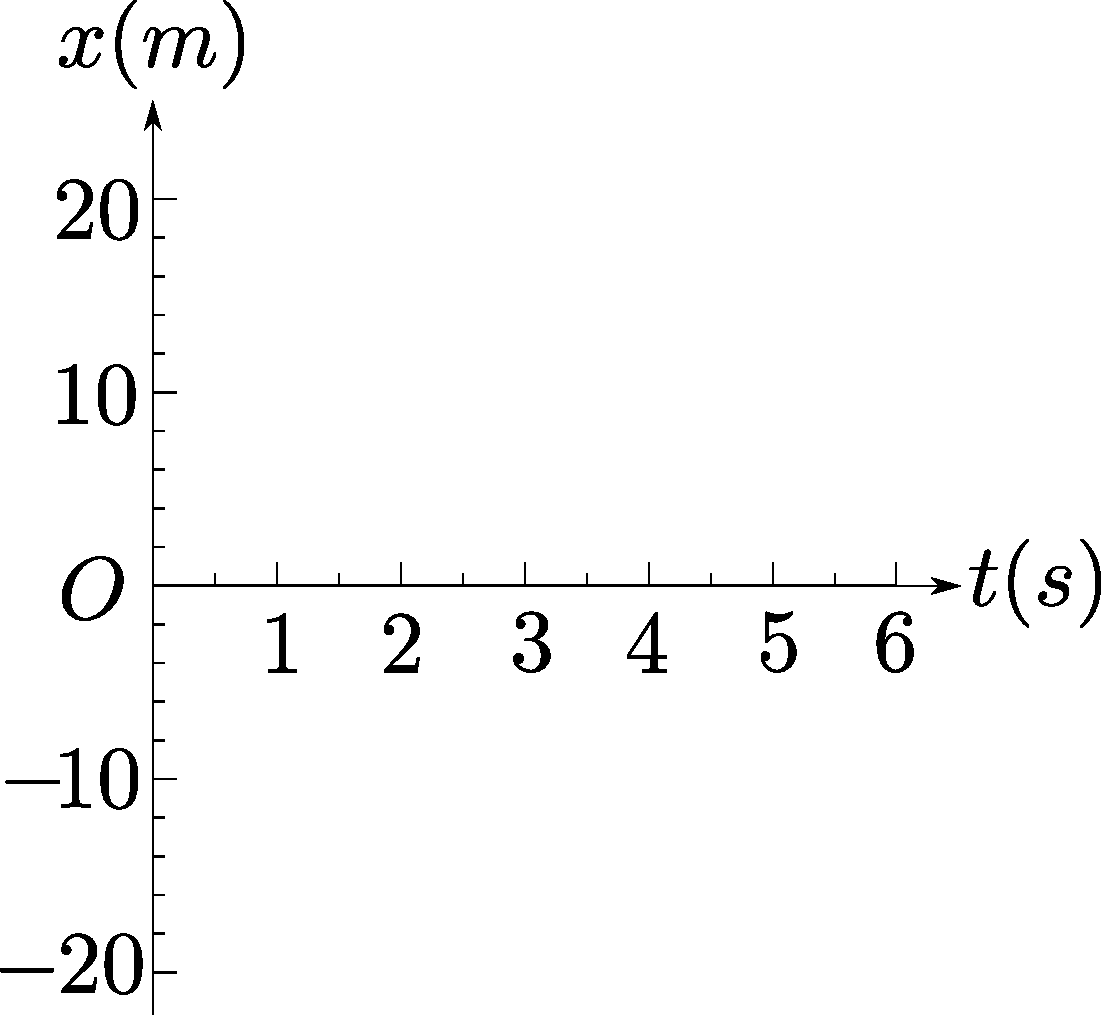
\includegraphics[width=0.5\textwidth]{images/motion-problem-empty-coordinate.pdf} 
\end{center}

\end{example}



\begin{example}
已知质点的运动可以用以下函数描写,在坐标系中画出其$x-t$图像。

(1): $x(t) = 5t^2$;(2):$x(t) = \frac{3}{t+1}$;(3):$x(t) = 5\sin(2\pi t)$
\begin{center}
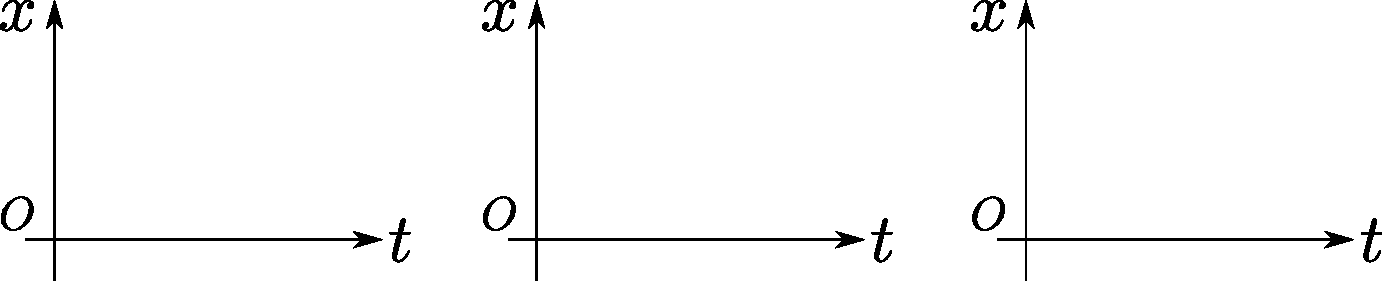
\includegraphics[width=0.9\textwidth]{images/motion-problem-three-empty-coordinate.pdf} 
\end{center}
\end{example}



\begin{example}
已知质点在一条直线上不同时刻的位置随时间的关系由下图给出,指出运动最明显的几个特征。
\begin{center}
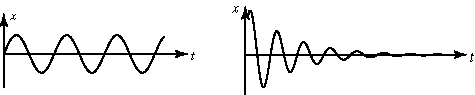
\includegraphics[width=0.8\textwidth]{images/motion-problem-4.pdf}
\end{center}
\tagged{student}{\vspace*{4cm}}
\begin{taggedblock}{teacher}
\noindent
解析:第一个就是简谐振动,第二个是阻尼振动,引导同学从图像中寻找尽可能多的信息。
\end{taggedblock}
\end{example}

事实上不但沿直线运动的质点可以利用以上的方法来描写,只要稍加思索就会发现用同样的方法来描写在弯曲的公路上行驶的汽车也是毫无问题的。
只需要在一条公路上找到一个正方向和原点,而行驶汽车的位置用它在公路上离开原点的距离来标记汽车的位置即可。
我国的公路里程就是用这种方法按照离开北京的距离进行统一标记的。


\subsection{运动的快慢:速率}
虽然当质点坐标随时间的函数为已知时,质点的运动的性质和特点实际上已经完全掌握了,但是我们还是希望从中得到运动有关的更为清楚的信息。
不同的物体运动快慢有着明显的不同,一个正常行走的人比乌龟要快很多,但与路上行驶的汽车比起来很明显要慢,物理上我们定义一个物理量--{\heiti 速率(speed)}来描写这种运动快慢的不同。
其实在过去已经有了一些速率的知识,那时将它称为速度,在物理上要格外注意两者的不同,这里我们谈的是速率,它用来给出运动快慢的量度。
只要想像一下行驶汽车的速率表,就能够马上得到关于速率的一个直观的印象。
过去速率定义为在某一给定的时间$ t$里运动质点所前进的路程,也就是距离$ s$的比值:
\begin{equation}
v = \frac{s}{ t}
\end{equation}
速率的这个定义对于匀速运动的质点来说没有问题,但是对于运动发生变化的过程来说就显得有些粗糙,比如对于静止开始逐渐加速的汽车来说。
很明显在开始的时候速率很慢,随着时间的增加速率则越来越快,为了更准确地描写物体运动的快慢我们需要更精确的速率的定义。
为此我们可以从某一时刻$t$开始计时,通过确定运动质点在某一不长的时间间隔$\Delta t$内前进的距离$\Delta s$与时间间隔$\Delta t$的比值称做在这一小段时间里质点运动的平均速率:
\begin{equation}\label{eqn: motion-平均速率的定义}
\overline{v} = \frac{\Delta s}{\dt}
\end{equation}
可以想像到的是选择越小的$\dt$,以如上方式得到的平均速率对运动质点在时间$t$时运动快慢的描写就越精确。

事实上$\dt$的选取是任意的,不同的$\dt$选取会得到不同的平均速率。
如果一个质点的运动用方程 $x=5t$ 来描写,那么对于任意的$t$,不同的$\dt$选取对平均速率实际上没有影响:
\begin{equation}
\overline{v} = \frac{5(t+\dt)-5t}{\dt} = \frac{5\dt}{\dt} = 5\unit{m/s}
\end{equation}
从运动方程来看我们也很清楚这时质点在做匀速运动,相同的时间里走过相同的距离。
但是如果另一个质点的运动方程为$x=5t^2$时,就不一样了,从函数的图像可以看出随着时间的增加看上去运动速度越来越快。
假如我们想知道在$t=1\unit{s}$时的速率,就需要在$t=1\unit{s}$时选择一个$\dt$并根据定义\ref{eqn: motion-平均速率的定义}来算出对于不同$\dt$时的平均速率。
\begin{eqnarray*}
\dt = 1&,&\overline{v} = \frac{5(1+1)^2-5}{1} = 15\unit{m/s}\\
\dt = 0.1&,&\overline{v} = \frac{5(1+0.1)^2-5}{1} = 10.5\unit{m/s}\\
\dt = 0.01&,&\overline{v} = \frac{5(1+0.01)^2-5}{1} = 10.05\unit{m/s}\\
\dt = 0.001&,&\overline{v} = \frac{5(1+0.001)^2-5}{1} = 10.005\unit{m/s}\\
\dt = 0.0001&,&\overline{v} = \frac{5(1+0.0001)^2-5}{1} = 10.0005\unit{m/s}\\
\dt = 10^{-n}&,&\overline{v} = \frac{5(1+10^{-n})^2-5}{1} = [10+5\pow{-n}]\unit{m/s} 
\end{eqnarray*}
从上面的计算可以很容易地看出,$\dt$取得越小所计算出的平均速率与$10\unit{m/s}$越接近,数学上将$\dt$取得小得不能再小时通过式\ref{eqn: motion-平均速率的定义}算出的运动质点在某一时刻到与它相邻极小时间里的平均速率称做运动质点在该时刻的{\heiti 瞬时速率}
\begin{equation}
v(t) = \lim_{\dt\rightarrow 0}\frac{\Delta s}{\dt}.
\end{equation}
行驶的汽车在每时每刻速率表的读数就是汽车在此时的瞬时速率。

当质点在某一时刻的瞬时速率为已知时,它在随后某一时间间隔$\dt$里所能够前进的距离就是瞬时速率$v$与时间间隔$\dt$的乘积
\begin{equation}\label{eqn: motion-ds=vdt}
\Delta s = v \dt.
\end{equation}
与瞬时速率的情况一样,$\dt$取得越小用这样的方式算出的前进距离与真实的前进距离的差别越小。
还以前面的运动$x(t)=5t^2$为例,已知在$t=1\unit{s}$时的瞬时速率$v = 10\unit{m/s}$,对于不同的$\dt$选取通过两种方法算出的前进距离分别为
\begin{eqnarray*}
\dt = 1,& \overline{v}\dt = 10\unit{m},&x(1+1)-x(1) = 15\unit{m}\\
\dt = 0.1,& \overline{v}\dt = 1\unit{m},&x(1+0.1)-x(1) = 1.05\unit{m}\\
\dt = 0.01,& \overline{v}\dt = 0.1\unit{m},&x(1+0.01)-x(1) = 0.1005\unit{m}\\
\dt = 10^{-n},& \overline{v}\dt = 10^{1-n}\unit{m},&x(1+10^{-n})-x(1) = [10^{1-n}+5\pow{-2n}]\unit{m}\\
\end{eqnarray*}
虽然有一些差别但是随着$\dt$变小,两者之间的差别就越来越小,虽然这种差别永远不会消失,但当$\Delta t\rightarrow 0$时用式\ref{eqn: motion-ds=vdt}来近似地表示质点前进的距离对于计算和分析都非常方便。


\begin{example}
下表为对于给定质点某一运动过程位置随时间关系的测量,求它在相邻两次测量之间运行的平均速率。

\begin{tabular}{|c|ccccccccccccc|}
\hline 
时间 & 0 & 0.5 & 1 & 1.5 & 2 & 2.5 & 3 & 3.5 & 4 & 4.5 & 5 & 5.5 & 6  \\ 
\hline 
位置 & 0 & 8.75 & 15 & 18.75 & 20 & 18.75 & 15 & 8.75 & 0 & -11.25 & -25 & -41.25 & -60 \\ 
\hline 
\end{tabular} 
\tagged{student}{\vspace*{4cm}}
\begin{taggedblock}{teacher}
\noindent
解析:注意这里求的是速率,所以要关注的是在给定时间段内走过的路程。
以1到1.5秒时间段为例,平均速率
\[
\overline{v} = \frac{18.75-15}{0.5} = \frac{3.75}{0.5} = 7.5\unit{m/s}
\]
其它时间段用相同的方法可以得到。
\end{taggedblock}
\end{example}

当在坐标系中谈论质点的运动时要特别注意的一点是,在建立坐标系的过程中我们已经假定了一个正方向,这样沿着坐标轴正方向的运动和沿着坐标轴负方向的运动虽然在相同时间里走过的路程是一样的,但经过一定的时间以后质点所处的位置却不同。
这一点在上面的例子当中也能够看出,从$t=0$到$t=2$的时间里,质点是沿着坐标轴的正方向运动,而在随后的时间里质点的运动方向则是与轴反向。
为了区别这种不同,在给出质点运动速率的同时就必须指出运动的方向,对于沿直线运动着的质点,沿着两个不同方向运动可以通过为速率指定一个正负号的办法达到。
当考虑了质点运动方向以后,速率就有了新的名称--{\heiti 速度(velocity)},对于沿轴运动着的质点,它的运动速度$v$能够为我们提供两个信息:质点本身移动的快慢用速度的绝对值给出,而移动的方向则由速度的正负号决定,当速度取正数时质点沿着轴正方向运动,反之当速度为负时质点则沿着轴的负方向运动。

对于一个以速度$v$匀速运动着的质点来说,如果$t$时刻它位于坐标轴上的$x_0$处,那么在此后的$\Delta t$时间之后,它所处位置的坐标$x$可以表达为
\begin{equation}
x = x_0 +v\Delta t
\end{equation}
无论质点的运动方向如何上式总是成立的。
对于那些不做匀速运动的质点,可以将$v$取做某一时刻的瞬时速度,那么对于越小的$\Delta t $的选取,由上式给出的坐标值就越精确。

\begin{example}
两个在同一直线上以匀速相向运动的质点$A$和$B$,在直线上建立坐标$Ox$,在开始时刻它们分别$x_A = -5\unit{m}$,$x_B=10\unit{m}$的位置。
已知质点$A$向着坐标正方向以$1.5\unit{m/s}$的速率运动,$B$逆着轴向运动,速率为$0.5\unit{m/s}$,求它们相遇的时间和位置。
 \tagged{student}{\vspace*{4cm}}
\begin{taggedblock}{teacher}
\noindent
解析:可能在小学就学过的相遇问题,是一个学习在坐标系中描写运动很好的例子。
两个质点的运动在坐标系中分别为
\[x_A = -5+1.5 t,\qquad x_B = 10-0.5 t\]
它们相遇时要求$x_A = x_B$,联立两个方程可以解出
\[t = 7.5\unit{s},\qquad x = -5+1.5\times 7.5 = 6.25\unit{m}\]
\end{taggedblock}
\end{example}

\subsection{图像详解}
\begin{figure}[htbp]
\begin{center}
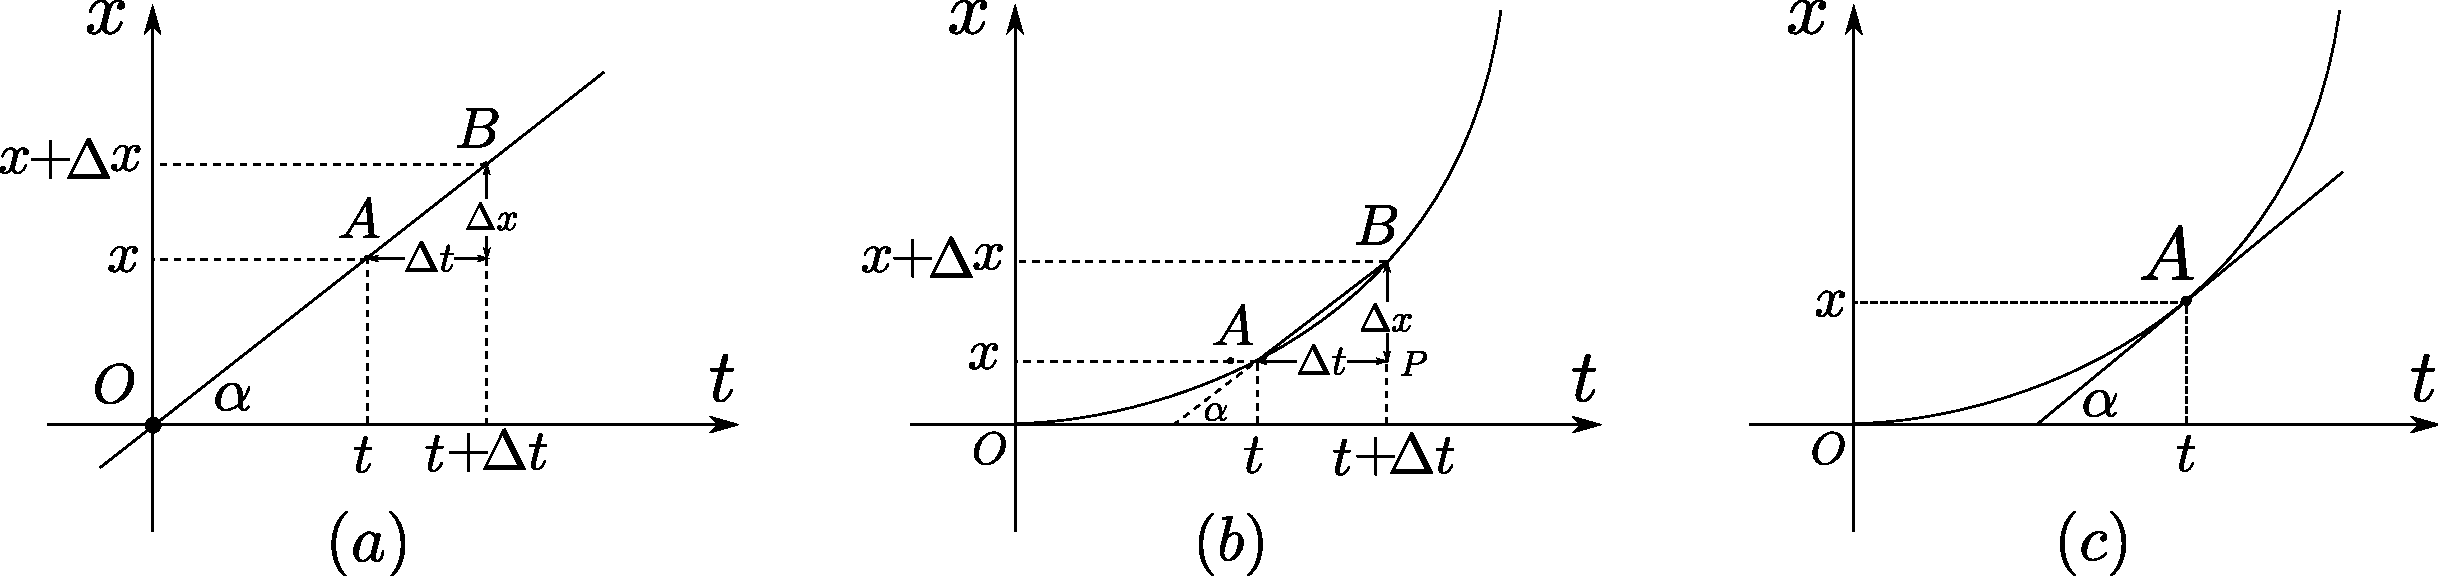
\includegraphics[width=0.8\textwidth]{images/motion-x-t.pdf}
\caption{一维运动$x-t$图像以及平均速率和瞬时速率的几何意义。(a)对于匀速直线运动来说,它的图像是一条直线,任意时刻的速率均为表示运动的直线的斜率。(b)一般运动过程中从$t$到$t+\Delta t$时间间隔中的平均速率,它是连接曲线上两点$A、B$构成的直线的斜率,直线上A、B两点之间的部分有时被称为曲线的割线。(c)当$\Delta t\rightarrow 0$时,B点和A点无限地接近,在图中已经无法区分两个点,这时用来衡量两个时间点里距离变化的割线也变成了曲线的切线,而切线的斜率正是运动物体在$t$时刻的瞬时速率。}
\label{fig: motion一维运动$x-t$图像以及平均速率的几何意义}
\end{center}
\end{figure}
无论是坐标,还是速度当质点运动时都能够用时间的某种函数来给出。
既然是函数,我们就可以将它们在坐标系中画出来,这样就可以很形象地看出运动函数所具有的性质,并且还能够得到不同物理量之间的联系。


最简单的图像自然就是坐标与时间的图像,有时称之为$x-t$图像,如图\ref{fig: motion一维运动$x-t$图像以及平均速率的几何意义}所示。
从图中可以很容易地找出某一给定时刻质点的坐标。
如果一个质点以匀速运动,那么它的$x-t$图像用图\ref{fig: motion一维运动$x-t$图像以及平均速率的几何意义}(a)中的直线表示,并且可以从图中看出质点运动的速率就是这条直线与横轴夹角$\alpha$的正切。

另外从$x-t$图像中其实我们还能够得到质点在某一时间段的平均速度,假设某一$t$时刻质点的坐标为$x$,它可以用图中的A点代表。
同理在时刻$t$之后一某个时间间隔$\dt$后它的坐标变成了$x+\Delta x$,可以用图中的B点来代表。
这样在$\dt$时间里的平均速率
\begin{equation}
\overline{v} = \frac{\Delta x}{\dt}
\end{equation}
就是图中直角三角形APB当中角$\alpha = \angle PAB$的正切。
对于越来越小的时间间隔$\dt$的选取,B点与A点的距离会越来越近,与此同时割线AB与曲线在A点的切线,就是那条与A点仅有一个交点的线产差别越来越小。
最终当B点无限地接近于A点时,割线AB就变成了曲线在A点的切线,而此时切线与横轴夹角的正切,也就是切线的斜率就是运动质点在此时的瞬时速率。






\begin{example}
根据如下x-t图像判断速度的变化趋势
\begin{center}
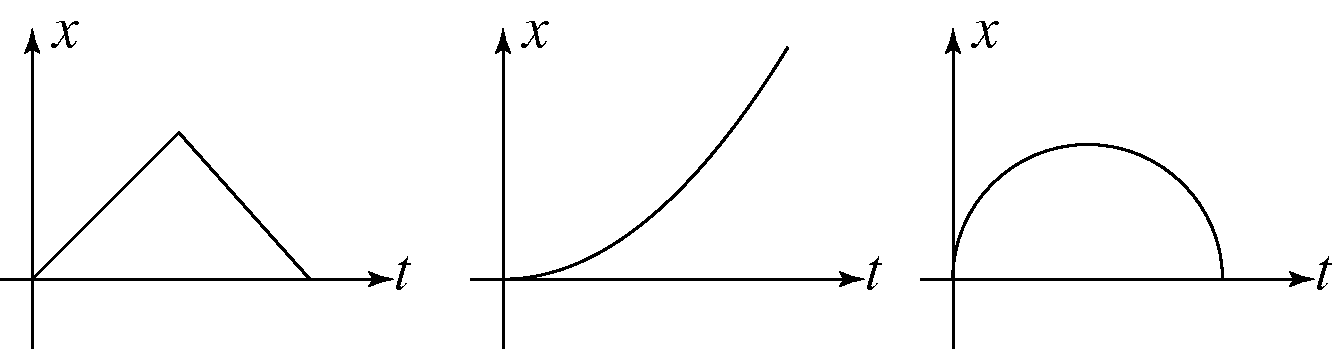
\includegraphics[width = 0.9\textwidth]{images/motion-problem-5.pdf}
\end{center}
\tagged{student}{\vspace*{3cm}}
\begin{taggedblock}{teacher}
\noindent
解析:根据图像分析即可,尽可能多提取出运动的信息。
\end{taggedblock}
\end{example}





\begin{figure}[h]
\begin{center}
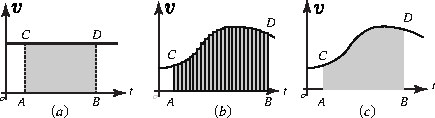
\includegraphics[width=0.8\textwidth]{images/motion-v-t.pdf}
\caption{一维运动$v-t$图像和运动距离的几何意义}
\label{fig: motion一维运动$v-t$图像以及运动距离的几何意义}
\end{center}
\end{figure}

除了$x-t$图像以外我们还可以做出$v-t$图像,也就是将不同时刻的速度用坐标系中的曲线连接起来,可以想像成在行驶的汽车里根据不同时刻速率表的读数。
当一个物体的运动速率不变时,它的$v-t$图像为一条平行一时间轴的一条直线,很明显一段时间里匀速运动质点前进的距离为速率与时间的乘积,图\ref{fig: motion一维运动$v-t$图像以及运动距离的几何意义}(a)当中矩形ABDC的面积就是由A到B点所代表的时间里质点前进距离。
当物体速率并不是常数而是随时间而变时,它的$v-t$图像如图\ref{fig: motion一维运动$v-t$图像以及运动距离的几何意义}(b)所示,其中轴坐标为对应时刻的瞬时速率。
根据\ref{eqn: motion-ds=vdt}式,质点在某一点处瞬时速率与之后一段微小时间间隔的乘积随着$\dt$取得越小则与真实运动在相同时间里所前进的距离越接近。
这样当给出$v-t$图像之后,物体前进的距离可以用图\ref{fig: motion一维运动$v-t$图像以及运动距离的几何意义}(b)当中很多宽为小的时间间隔,高为对应时刻的瞬时速度构成的窄矩形的面积的和。
可以看出,这些窄矩形的面积和在$\dt$越来越小时与图\ref{fig: motion一维运动$v-t$图像以及运动距离的几何意义}(c)当中由ABDC四个点围成区域的面积越来越接近!
也就是说,当给出$v-t$图像以后一段时间里质点前进的距离为$v-t$图像在两个时间点之间与横轴包围的曲线的面积。



\begin{example}
若质点作直线运动的速度$v$随时间$t$变化的图像如下图所示,则该质点的位移$x$(从$t=0$开始)随时间$t$变化的图像可能是下面的哪一个?
\begin{center}
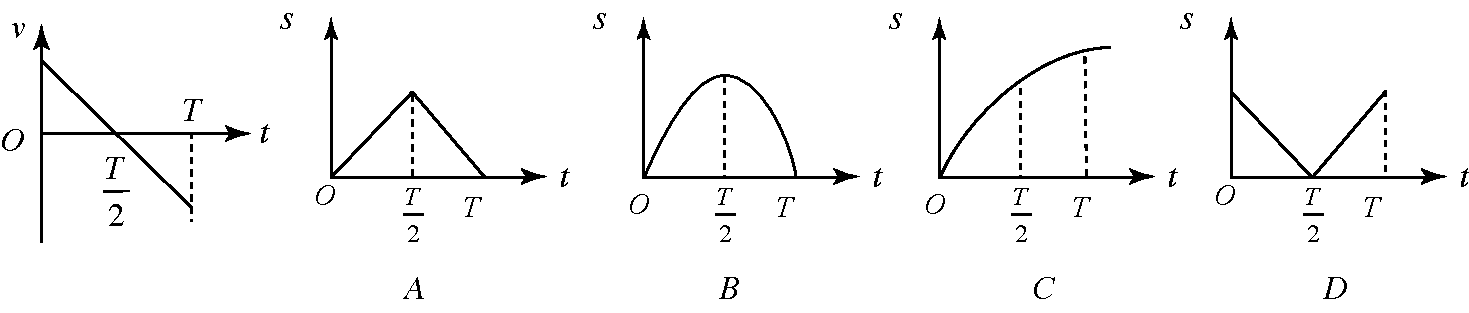
\includegraphics[width=0.9\textwidth]{images/motion-problem-39.pdf}

\end{center}
\tagged{student}{\vspace*{1cm}}
\begin{taggedblock}{teacher}
\noindent
解析:位移先变大后变小,开始时刻位移为零,根据图像可知最终位移也是零,所以答案是$B$。
\end{taggedblock}
\end{example}

\begin{example}
求质点在用以下 $v-t$图所表示的运动过程当中从初始时刻$t=0$出发到图中给定的$t$时刻当中所走过的总路程。
\begin{center}
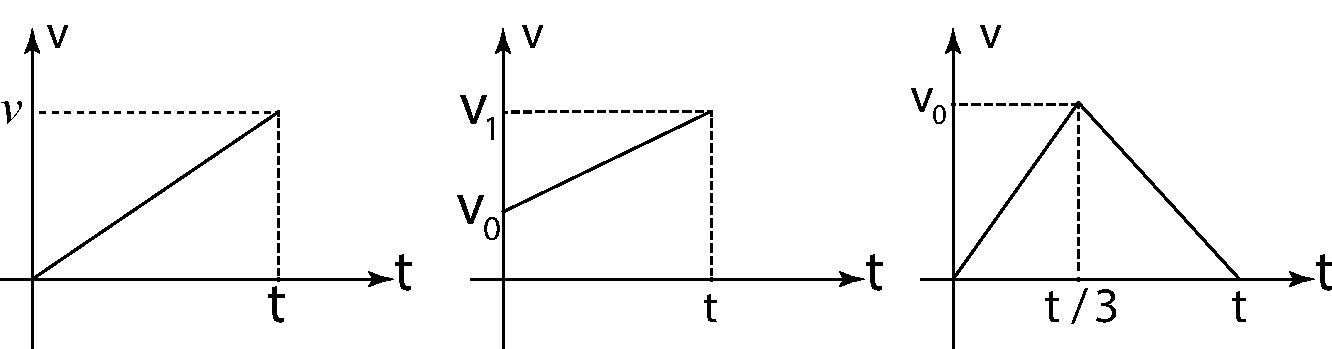
\includegraphics[width = 0.9\textwidth]{images/motion-problem-6.pdf}
\end{center}

\tagged{student}{\vspace*{4cm}}
\begin{taggedblock}{teacher}
\noindent
解析:所有的运动速度方向不变,所以$v-t$图像与$x$轴围成的面积就是走过的路程,这样
\begin{eqnarray*}
S_1 &=& \frac{1}{2}vt\\
S_2 &=& \frac{1}{2}(v_0+v_1)t\\
S_3&=& \frac{1}{2}v_0t
\end{eqnarray*}

\end{taggedblock}
\end{example}




\subsection{加速度,匀加速运动}
一般来说一个质点的运动速率总是在不断地发生变化,只要想像一辆行驶在路上的汽车就能够得到这样的印象。
正是因为这一点引入一个物理量来描写速率变化的快慢是很有必要的。
假设一个质点在某一时刻$t$的速率为$v(t)$,而在此后的$\dt$间隔之后由于某种原因变成了$v(t+\dt)$,在这个运动过程中速率的增加量自然就是$\Delta v = v(t+\dt)-v(t)$,那么加速度就被定义为速率的变化量与发生这一速率变化所需要时间$\dt$的比值:
\begin{equation}\label{eqn: motion-加速度的定义}
a = \frac{\Delta v}{\dt} = \frac{ v(t+\dt)-v(t)}{\dt}.
\end{equation}
很明显,如果在给定时间里速率变化量越大就对应着较大的加速度,反之若在相同的时间里速率只发生了很小的改变,那么意味着较小的加速度。
物理上用{\heiti 加速度(acceleration)}来衡量速度变化的快慢和方式。
如果上式中的间隔$\dt$是一个相对较大的时间,在该时间前后速度发生了相当可观的变化,那么由上式定义出的加速度就是$\dt$时间里的{\heiti 平均加速度}。
而当$\dt$取得非常之小,就可以认为由上式得到的实际上是运动质点在$t$时刻的{\heiti 瞬时加速度}。

当在一段时间里质点运动的加速度保持不变,这样的运动就被称为{\heiti 匀加速运动}。
若加速度为$a$且不随时间而变,在$t=0$的时刻质点的初始速率为$v_0$,那么在此之后的任意时刻$t$质点运动的速率则是
\begin{equation}\label{eqn: motion-v=v0+at}
v(t)=v_0+at.
\end{equation}
可以看出速度随时间线性增加,此时的$v-t$图像由图所示。
我们知道$v-t$图像在给定的两个时间点下包围的面积就是在该时间间隔当中质点的路程,当质点初始坐标为$x_0$时此后任意$t$时间它的坐标则是
\begin{equation}\label{eqn: motion=x=x0+v_0t+1/2at^2}
x(t)=x_0+v_0t+\frac{1}{2}at^2.
\end{equation}

和速度一样,加速度也可用它与时间的图像来形象地给出,匀加速度运动质点的$v-t$图像是一条直线,根据前面的经验可知加速度对应于该直线与时间轴夹角的正切,也就是该直线的斜率。
对于一般的情况,在任意时刻$t$加速度则是$v-t$曲线在该点处切线的斜率。
反过来当给出$a-t$图像时,两个给定时间之间$a-t$曲线下的面积则对应于这一段时间里速度的变化量。


\begin{example}
根据速度-时间图像由\ref{eqn: motion-v=v0+at}推出匀加速运动中位置随时间的变化关系式\ref{eqn: motion=x=x0+v_0t+1/2at^2}。
\tagged{student}{\vspace*{4cm}}
\begin{taggedblock}{teacher}
\newline
解析:匀加速度运动的$v-t$图像是直线,所以位移就是直线与横轴围成的面积,这样我们就有
\[
x(t)-x_0 = \frac{1}{2}(v_0+v_0+at)t = v_0t+\frac{1}{2}at^2,
\]
移项就可得证。
\end{taggedblock}
\end{example}

\begin{example}
加速度$a$作匀加速运动的质点初速度$v_1$,位置为$x_1$,在经过一段时间以后它的速度变成了$v_2$,运动到了坐标轴上的$x_2$处,证明以上物理量之间满足关系式
\[
v_2^2-v_1^2=2a(x_2-x_1)
\]
\tagged{student}{\vspace*{4cm}}
\begin{taggedblock}{teacher}
\noindent
解析:匀加速运动过程速度、位置随时间的变化规律分别为
\[v_2=v_1+at,\qquad x_2=x_1+v_1 t+\frac{1}{2}at^2\]
由第一个式子解出时间$t$得到
\[
t = \frac{v_2-v_1}{a}
\]
代入第二个式子就可以从两个方程当中消去时间,得到位置、速度和加速度之间的关系
\[
x_2-x_1 = v_1\frac{v_2-v_1}{a}+\frac{1}{2}a\frac{(v_2-v_1)^2}{a}
\]
将上式化简之后就可证明上述关系。
\end{taggedblock}
\end{example}

%%%%%%%%%%%%%%%%%%%%%%%%%%%%%%%%%%
\begin{example}
一列火车以给定的加速度沿直线轨道前进。
当列车前端通过点$O$时,列车的速度为$u_1$,当列车尾端通过$O$点时,速度为$u_2$,试求列车中部通过$O$点时的速度$v$。
\tagged{student}{\vspace*{4cm}}
\begin{taggedblock}{teacher}
\newline
解析:设列车长度为$L$,加速度为$a$,根据前面的公式我们有
\[
u_2^2-u_1^2 = 2aL,
\]
当中点通过时走过的路程是列车总长的一半,所以
\[
v^2-u_1^2 = 2a\frac{1}{2}L = aL = \frac{u_2^2-u_1^2}{2},
\]
整理之后可得
\[
v^2 = \frac{1}{2}(u_1^2+u_2^2),\qquad v = \sqrt{\frac{1}{2}(u_1^2+u_2^2)}.
\]
\end{taggedblock}
\end{example}
%%%%%%%%%%%%%%%%%%%%%%%%%%


\begin{example}
一辆汽车在公路上以速度$v_0 = 20\unit{m/s}$沿直线行驶,当它到达路口前$60\unit{m}$处发现交通信号的倒计时还剩$2\unit{s}$,如果他想加速通过路口,所需的加速度至少为多少?
如果他不想闯红灯,停止所需要的加速度至少为多少?
\tagged{student}{\vspace*{4cm}}
\begin{taggedblock}{teacher}
\newline
解析:若想通过路口,必须在2s内走完剩下的60m,设加速度为$a_1$,如果刚好通过,需要有
\[
v_0 t +\frac{1}{2}a_1t^2 = 60,\qquad a>a_1 = 10\unit{m/s^2}
\]
反之要想停下来,根据实际情况,对运动的时间没有要求,而是要在60m内停下来,设刚好停下来的加速度为$a_2$
\[
0-v_0^2 = 2a_2L,\qquad a<a_2 \simeq -3.3\unit{m/s^2}
\]
\end{taggedblock}
\end{example}

\begin{example}
A火车以$v_1=20\unit{m/s}$的速度匀速行驶,司机发现前方同轨道上相距$100\unit{m}$处有另一列火车正以$v_2=10\unit{m/s}$的速度匀速行驶,$A$车立即做加速度大小为$a$的紧急制动。
求能够使两车不至于相撞的$a$的最小取值。
\tagged{student}{\vspace*{4cm}}
\begin{taggedblock}{teacher}
\newline
解析:建立以火车$A$发现前车时刻$A$的位置为原点的坐标系,设$A$的加速度为$a$,两车的运动方程分别为
\[
x_A = v_1t+\frac{1}{2}at^2,\qquad x_B = 100+v_2t,
\]
如果两车不会相撞,那么意味着方程$x_A = x_B$无解:
\[
\frac{1}{2}at^t+(v_1-v^2)t-100 = 0,\qquad \frac{1}{2}at^t+10t-100 = 0
\]
二次方程无解要求判别式小于零:
\[
\Delta  = 100+200a<0,\qquad a<0.5\unit{m/s^2}
\]
\end{taggedblock}
\end{example}




\begin{example}
在通过某一弯道之后的大直道上两辆赛车展开追逐,后车的速度为$v_1$,前车的速度$v_2>v_1$,后车具有更好的加速性能$a_1>a_2$,两车相距$d$且直道的全长为$L$。
简单起见将两辆车都看成质点,求后车能够在直道上超越前车的条件。
\tagged{student}{\vspace*{4cm}}
\begin{taggedblock}{teacher}
\newline
解析:以后车的位置为原点建立坐标系,这样两车的运动可写为
\[
x_1 = v_1t+\frac{1}{2}a_1t^2,\qquad x_2 = d+v_2t+\frac{1}{2}a_2t^2
\]
不考虑赛道长度的情况下一定可以追上,追上的时间由方程$x_1=x_2$给出,它的解为
\[
t = \frac{(v_2-v_1+\sqrt{(v_2-v_1)^2+2(a_2-a_1)d})}{a_1-a_2},
\]
如果考虑了赛道的长度,就要求在上式解的时刻后面赛车走过的路程小于总长:
\[
v_1t+\frac{1}{2}a_1t^2<L,
\]
这样就可以给出能够追上所满足的条件。
\end{taggedblock}
\end{example}





\subsection{落体运动}
将一个重物由静止释放以后的运动就是一种均加速运动,以这种方式运动的物体称为{\heiti 自由落体}。
为了和今后的表达方式一致,建立一个竖直向上的坐标系$x$,物体由坐标系的原点处静止释放,实验表明任何自由落体都以相同的加速度均加速下落,加速度指向地面,随着时间的推移其速率均匀增加
\begin{equation}
v(t) = -gt,
\end{equation}
位置随时间的关系则是
\begin{equation}
x(t) = -\frac{1}{2}gt^2,
\end{equation}
其中$g\simeq 9.8 \unit{m/s^2}$,称为地球表面的{\heiti 重力加速度}。


当初始时刻$t=0$时速度或坐标取非零值时自由下落物体速度和位置随时间的变化关系由一般情况下的均加速运动满足的规律给出。
如果$t=0$时自由落体的位置和速度分别为$x_0$和$v_0$时,此后它的速度和位置随时间的关系为
\begin{equation}
v(t) = v_0-gt,\qquad x(t) = x_0+v_0t-\frac{1}{2}gt^2.
\end{equation}

\begin{example}
将竖直向上的坐标轴原点取成抛出物体的那一点,在以下各种情况下求质点的坐标:

(1)由静止开始下落的质点$1\unit{s}$、$5\unit{s}$、$10\unit{s}$时。

(2)向上以初速度$v_0=10\unit{m/s}$抛出质点在$1\unit{s}$、$2\unit{s}$、$3\unit{s}$时。

(3)向下以初速度$v_0=10\unit{m/s}$抛出质点在$1\unit{s}$、$2\unit{s}$、$3\unit{s}$时。
\tagged{student}{\vspace*{4cm}}
\begin{taggedblock}{teacher}
\newline
解析:三种情况下的运动方程分别为
\[
x_1 = -\frac{1}{2}gt^2,\qquad x_2 = 10t-\frac{1}{2}gt^2,\qquad x_3 = -10t-\frac{1}{2}gt^2,
\]
将各个时刻代入即可。
\end{taggedblock}
\end{example}

\begin{example}
建立竖直向上的坐标系$x$,从原点出发以初速度$v_0 = 20\unit{m/s}$竖直上抛的一个质点,质点的$x$坐标值就相当于抛出以后运行的高度。
求它运动到高度分别为 15 m、20 m 、25 m 、0 m 、-25m处所需要的时间。
为简单起见设$g=10 \unit{m/s^2}$
\tagged{student}{\vspace*{4cm}}
\begin{taggedblock}{teacher}
\newline
解析:设希望知道时间的高度为$h$,那么到达该高度的时间由方程
\[
h = 20t-5t^2,\qquad  5t^2-20t+h = 0
\]
给出,将各个高度代入上式求解二次方程即可得到时间:
\begin{enumerate}
\item x=15 m: 方程$5t^2-20t+15=0$,有两个解$t=1s,3s$,分别对应于上升阶段和下降阶段到达该高度的时间。
\item x=20 m: 方程$5t^2-20t+20=0$, 只有一个解$t=2s$,意味着到达最高点。

\item  x=25 m: 方程$5t^2-20t+25=0$,判别式小于零,无解,意味着给定的初速度飞不了这么高。

\item x=0m: 方程$5t^2-20t=0$, 两个解$t=0,4$,一个解对应于扔出的时刻,一个解对应于再次落回来的时刻。

\item x=-25m: 方程$5t^2-20t-25=0$,两个解$t=5,-1$,一个解正是落回来的时刻,另一个解对应于过去的时间,意味着一个在更低的点抛出物体,它正好在$t=0$的时刻通过这里的坐标原点且速度刚好是向上$20\unit{m/s}$的物体,它在上升过程中到达原点下方$25\unit{m}$处的时间,自然它对应于$t<0$的时间。
\end{enumerate}
\end{taggedblock}
\end{example}

\begin{example}
如图所示在地面上方高度为$h$处有一个质点$A$自由下落的同时从地面以初速度$v_0$竖直上抛另一个质点$B$,求它们能够在空中相遇的最小上抛速度$v_0$。
\begin{flushright}
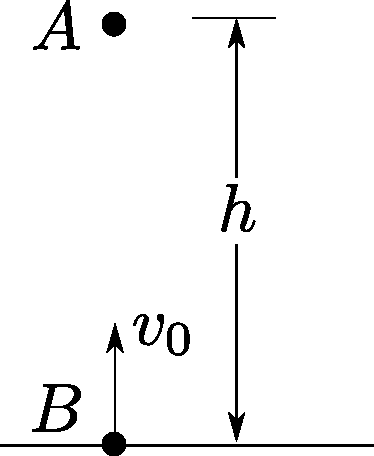
\includegraphics[width = 0.2\textwidth]{images/motion-one-up-one-down.pdf} 
\end{flushright}
\tagged{student}{\vspace*{1cm}}
\begin{taggedblock}{teacher}
\noindent
解析:建立一个原点在地面竖直向上的坐标系$Ox$,两个质点的运动方程分别为
\[x_A= h-\frac{1}{2}gt^2,\qquad x_B = v_0 t-\frac{1}{2}gt^2\]
设它们将于时刻$t$相遇,$t$满足方程
\[x_A = x_B,\qquad h = v_0 t,\qquad t=\frac{h}{v_0}\]
这么长的时间里$A$下落的高度必须小于$h$,这样它们才能够在空中相遇:
\[
\frac{1}{2}gt^2=\frac{1}{2}g(\frac{h}{v_0})^2\le h
\]
很容易解出$v_0$必需满足条件
\[ v_0^2\le \frac{1}{2}gh\]
\end{taggedblock}
\end{example}

\begin{example}
一个女子从高楼上落下,超人于时间$T$之后发现了这件事,超人立即以初速度$v_0$加速向下飞去救该女子。
假设女子下落和超人的飞行作自由落体运动,假设楼高$H$,求超人能够在女子落地前将她救起的最小初速度$v_0$。

\tagged{student}{\vspace*{4cm}}
\begin{taggedblock}{teacher}
\noindent
解析:选择超人发现以后的时刻为计时的起点,坐标系从楼顶算起竖直向下,开始时刻女子的速度$gT$,位置$\frac{1}{2}gT^2$,两者的运动方程分别为
\[
x_S = v_0t+\frac{1}{2}gt^2,\qquad x_g = \frac{1}{2}gT^2+gTt+\frac{1}{2}gt^2
\]
两人能够在空中相遇需要他们的坐标一致并且超人走过的距离比楼高要小。
简单的计算表明他们相遇的时间
\[
t = \frac{\frac{1}{2}gT^2}{v_0-gT},
\]
可见如果$v_0<gT$则无论如何也追不上,反之如果能够追上,那么追上时超人下降的高度
\[
h = v_0t+\frac{1}{2}gT^2 = \frac{1}{2}gT^2\frac{v_0^2-gTv_0-\frac{1}{4}g^2T^2}{(v_0-gT)^2} = \frac{1}{2}gT^2\frac{(v_0-\frac{1}{2}gT)^2}{(v_0-gT)^2}<H,
\]
经过计算可解出
\[
v_0>gT\frac{\sqrt{\frac{2H}{gT^2}}-\frac{1}{2}}{\sqrt{\frac{2H}{gT^2}}-1}
\]
\end{taggedblock}
\end{example}

\begin{example}
一质点自距离水平地面高$H$处自由下落,每次与地面发生碰撞以后反弹的速率均为撞向地面速率的$e$倍,$e<1$。
求自第一次反弹以后算起到最终停止所需要的总时间和质点走过的总路程。
\begin{flushright}
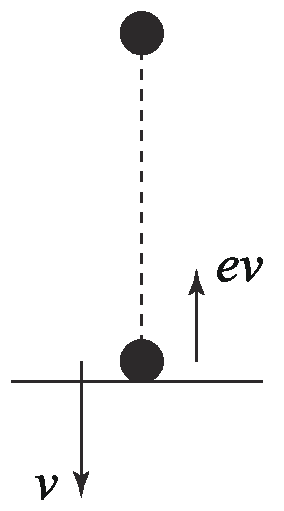
\includegraphics[width = 0.2\textwidth]{images/motion-29.pdf} 
\end{flushright}
\tagged{student}{\vspace*{0cm}}
\begin{taggedblock}{teacher}
\noindent
解析:第一次反弹之前质点撞向地面的速率$v_0 = \sqrt{2gH}$。
第一次反弹之后其向上的速率变成$v_1=ev_0$,上升到下落所需要的总时间$t_1 = \frac{2v_1}{g} = 2e\frac{v_0}{g}$,到第二次撞向地面之前走过的总路程$s_1 = e^2\frac{v_0^2}{g} = e^2H$。
很容易将这些结论推广到随后的情况,这样到最终停止时所经历的总时间
\[ T = \sum_{n=1}^\infty t_n =  \frac{2v_0}{g}\sum_{n=1}^\infty e^n = \frac{2v_0}{g} \frac{e}{1-e}  = 2 \sqrt{ \frac{2H}{g}} \frac{e}{1-e},\]
同样的道理到最终停止所走过的总路程则是
\[  S = \sum_{n=1}^\infty s_n =  H \sum_{n=1}^\infty e^{2n} = H\frac{e^2}{1-e^2}.\]
它们都是有限的,这一点从直观上不太容易发现。
\end{taggedblock}
\end{example}


%%%%%%%%%%%%%%%%%%%%%%%%%%%%%%%%%%
\begin{example}
一个质点以初速度$v_0$撞向一个板,第一次与板碰撞反弹以后的运动变成加速度指向板的匀加速运动,加速度大小为$a$,此后每次与板碰撞以后速度反向且大小不变,但指向板的加速度变成原来的$k(k>1)$倍。
求此后运动的总时间和质点走过的总路程。
\tagged{student}{\vspace*{4cm}}
\begin{taggedblock}{teacher}
\newline
解析:和前一问一样的思路,第一次反弹以后的运动记做第0次运动,这样就有递推关系:
\[  a_n = k^na,\qquad t_n = \frac{1}{k^n}\frac{2v_0}{a},\qquad s_n = \frac{1}{k^n}\frac{v_0^2}{a},\]
这样总时间和总路程为
\[
T = \sum_{n=0}^\infty t_n = \frac{2v_0}{a}\frac{k}{k-1},\qquad S = \sum_{n=0}^\infty s_n = \frac{v_0^2}{a}\frac{k}{k-1}.
\]
\end{taggedblock}
\end{example}
%%%%%%%%%%%%%%%%%%%%%%%%%%%%%%%%%%

\begin{example}
有一竖直放置、两端封闭的长玻璃管,管内为真空,管内有一小球自某处自由下落(初速度为零),落到玻璃管底部时与底部发生弹性碰撞,反弹速度与入射速度相同。
以后小球将在玻璃管内不停地上下跳动。
现在支架固定一照相机,用以拍摄小球在空间的位置。
每隔一相等的确定的时间间隔$T$拍摄一张照片,照相机的曝光时间极短,可忽略不计。
从所拍到的照片发现,每张照片上小球都处于同一位置。
求小球开始下落处离玻璃管底部距离(用$H$表示)的可能值以及与各$H$值相应的照片中小球位置离玻璃管底部距离的可能值。
\tagged{student}{\vspace*{6cm}}
\begin{taggedblock}{teacher}
\newline
解析:全国中学生物理竞赛复赛
\end{taggedblock}
\end{example}



\section{高维运动,位移,速度}
前面我们研究的都是做一维运动的质点,定义了位置(坐标),速度和加速度等能够方便描写质点运动的物理量。
当质点的运动并不局限于一条直线或给定的轨道上时,描写它的运动通常要更复杂一些,需要一些新的概念和物理量才能做到。
大多数情况下,尽管质点的运动不在一条直线上,但依然保持在某一个给定的平面中,例如抛体的运动以及地球围绕太阳的公转都满足这一特征,所以我们首先来看一下在一个平面中的运动,当搞明白平面内的运动以后很容易向三维空间运动做推广。
\subsection{位置的确定:坐标系}
在一个平面上确定一个点的位置比在直线上需要更多的信息。
生活上有两种常用的方法来说明两点之间的位置关系,例如说清华大学在从天安门出发向西走6公里再向北走11公里;或者说北京大学在天安门北偏西大约40$^\circ$方向12公里处。
这两种描述方法对应于物理中的两种常用的方式来确定平面上一个点的位置。
\begin{enumerate}
\item 直角坐标系:  如图\ref{fig: motion-两种坐标系}(a)所示,从一个给定点$O$出发沿着两个相互垂直的方向做两个数轴$x,y$,那么任意点的位置可以用它在这两个轴上的投影的坐标值$(x,y)$唯一确定。
当一个点的$x$坐标取负值时说明它在$O$点的左侧,同理当它的$y$坐标值为负数时说明它在$O$点的下方,$x、y$坐标可能的取值范围都是全部的实数值。
\item 平面极坐标系:如图\ref{fig: motion-两种坐标系}(b)所示的从一个给定点$O$出发确定一个给定的方向$ON$,任何一点P的位置用它和$O$点的直线距离$r$以及和给定方向之间的夹角$\theta$来唯一确定。
与直角坐标系不同的是$r$的取值范围是从0开始的正数,$r=0$意味着该点位于图中的$O$点处;角度变量$\theta$的取值有一定的任意性,从角度的一般定义可以看出,对于相同的$r$,当两个角度$\theta_1$和$\theta_2$相差$2\pi$的整数倍时实际上对应于图中的同一个点,在使用的时候要注意这一点。
另外原点$O$处的角度取值并没有实际意义,都对应于图中的$O$点。
\end{enumerate}




\begin{figure}[hbtp]
\centering
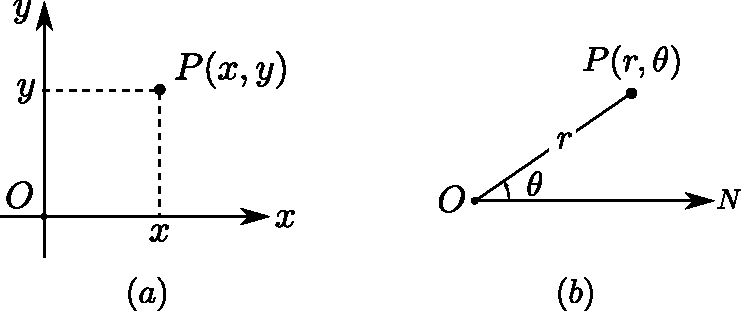
\includegraphics[width=0.6\textwidth]{images/motion-theory-1.pdf}
\caption{(a)平面直角坐标系, (b)平面极坐标系}\label{fig: motion-两种坐标系}
\end{figure}

无论选取哪种坐标系来描写质点的运动,都必须在开始描写物理问题之前明确地指出坐标系的取法。
对于直角坐标系来说需要指出原点的位置以及两个轴的正方向分别指向何处;当使用平面极坐标系时需要 指定原点的位置和参考方向的取向,只有当坐标系被明确地给出以后利用坐标系来描写质点的运动才是有意义的。
两种坐标系都可用来唯一地给出质点的位置,在处理不同问题时选择合适的坐标系会使问题极大地简化。
一般来说研究地球上质点的运动时选用直角坐标系来描写质点的位置,但是如果运动有一个明显的中心,例如太阳系中各个行星围绕太阳的转动时用极坐标则会更方便一些。

\begin{example}
在下图所示的平面直角坐标系中标出由以下几个已知坐标的点:

$A:  (3,4); B: (5,0); C: (-3,2);  D: (2,-5); E: (-3,-2); F: (0, 3); G: (-1,0); H: (0,-3) $
\begin{center}
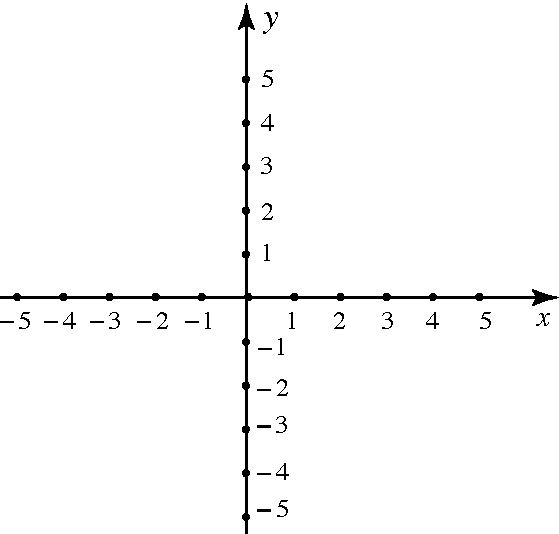
\includegraphics[width=0.4\textwidth]{images/motion-problem-7.pdf}
\end{center}

\tagged{student}{\vspace*{0cm}}
\begin{taggedblock}{teacher}


\end{taggedblock}
\end{example}

\begin{example}
在下图所示的平面极坐标系中标出由以下几个已知坐标的点:

$A: (5, \pi/3); B: (2, \pi/3);  C:(5, \pi/2); D:(4, \pi); E: (4, 3\pi/2)), F: (3,0)$
\begin{center}
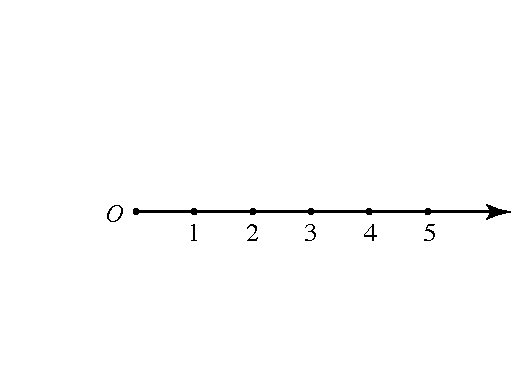
\includegraphics[width=0.4\textwidth]{images/motion-problem-8.pdf}
\end{center}
\tagged{student}{\vspace*{0cm}}
\begin{taggedblock}{teacher}


\end{taggedblock}
\end{example}

\subsection{位置的变化:位移}
当质点在平面上运动,也就是它的位置发生变化时,描述这种变化一般我们会说“它从某处(起点)出发沿着某种路线(轨迹)最后到达了某处(终点)”。
如图\ref{fig: motion-始末点相同但沿着不同路径的运动}所示对于相同的起点$A$和终点$B$会有无数种运动的轨迹(path),沿着不同轨迹的运动很不一样,但它们都有共同的起点和终点。
物理上我们用{\heiti 位移(displacement)}来描写运动质点的位置变化,它的定义很简单,就是一条由起点到终点的一个箭头,即有向线段来给出质点的位移。
这个有向线段的长度代表了位置变化的距离,而它的方向自然给出了位置变化的方向。
这样当初始位置为已知,并且经过某种运动之后的位移也为已知时,在运动结束以后的位置就被唯一确定了。
图\ref{fig: motion-点出发沿给定路径运动到不同位置时质点的位移}给出了从A点出沿着曲线运动的质点在各个不同位置时的位移。
从中可以看出,如果两点非常接近时,位移的大小和质点真正走过的距离非常接近,但当质点沿着轨迹前进一段距离之后位移的大小和所走过路程之间有了明显的差别,并且位移的大小和所走过路程的长短也没有必然的关系。


\begin{figure}[hbtp]
\begin{minipage}[c]{0.45\textwidth}
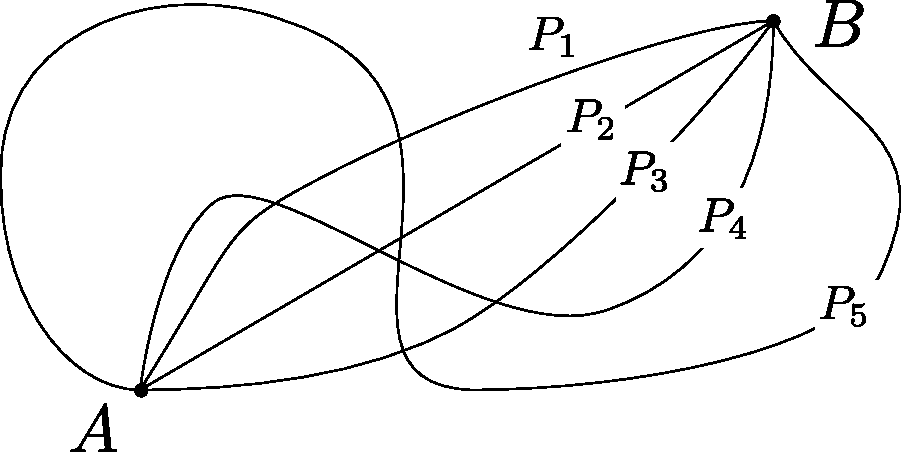
\includegraphics[height=1in]{images/motion-theory-2.pdf}
\caption{始末点相同但沿着不同路径的运动}
\label{fig: motion-始末点相同但沿着不同路径的运动}
\end{minipage}
\begin{minipage}[c]{0.45\textwidth}
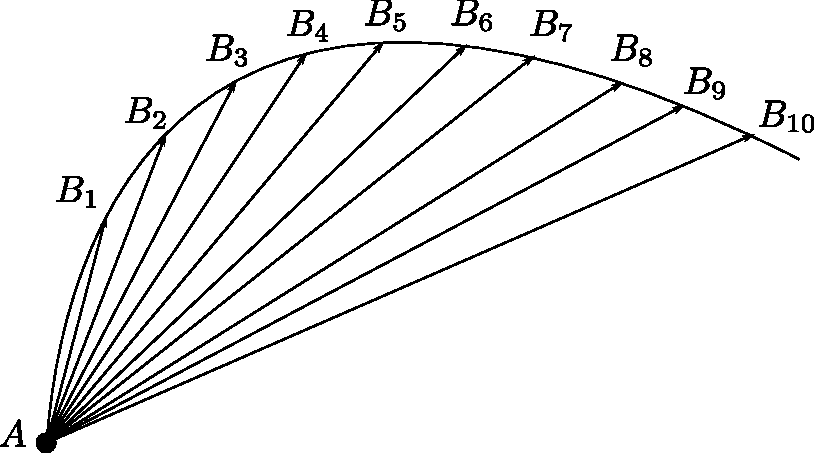
\includegraphics[height=1in]{images/motion-theory-3.pdf}
\caption{从$A$点出发沿给定路径运动到不同位置时质点的位移}
\label{fig: motion-点出发沿给定路径运动到不同位置时质点的位移}
\end{minipage}
\end{figure}

除了用箭头来表示位移,其实我们还可以用一段运动过程前后质点在给定坐标系中坐标值的变化来表示给定过程中的位移。
对于一个在给定平面内运动的质点,建立一个平面直角坐标系$Oxy$,当它在运动开始时刻位于由坐标$(x_1,y_1)$所给出的位置,而在运动结束时的位置为$(x_2,y_2)$时,整个运动过程的坐标变化量:
\[\Delta x = x_2-x_1,\qquad \Delta y = y_2-y_1\]
也可以用来表示其位置移动。
反过来,对于初始时刻位置$(x_1,y_1)$和一段运动过程中的位置变化$(\Delta x,\Delta y)$为已知时,运动结束时刻的位置$(x_2,y_2)$可以利用以上两个物理量求出:
\[x_2 = x_1+\Delta x,\qquad y_2 = y_1+\Delta y.\]

\subsection{具有大小的方向的物理量:矢量}
像位移这样的物理量我们以前很少接触,不但需要有给定的大小同时还需要给出它的方向才能够完全确定一个质点的位移。
物理上将这种必须由大小和方向同时决定的物理量称做{\heiti 矢量(vector)};与之相对应的那些只需要给出大小就可以完全给出的物理量被称为{\heiti 标量(scalar)}。既然矢量由大小和方向来给出,直观地描写一个矢量需要要在纸上画出矢量的大小和方向。
因为矢量同时具有大小和方向,所以当我们说两个矢量相等时不但要求它们的大小相等,同时也必须指向相同的方向才可以。



对于一个给定的矢量和另外一个标量(数),可以定义标量和矢量的乘积,它们的乘积同样是一个矢量,方向与被乘的矢量完全一致,而大小则为被乘矢量的大小与标量大小的乘积,需要注意的是当标量乘数为一个负数时,相乘的结果矢量方向与被乘矢量相反!
类似地可以定义一个矢量除以一个标量为矢量和标量倒数的乘积,只要该标量不为零的话。

如果有两个给定的矢量$\vec{A}$和$\vec{B}$,定义两者的加法:将$\vec{B}$的起点放置在$\vec{A}$的终点处,那么两者相加的结果为一个新的矢量$\vec{C}$,它是一个由$\vec{A}$的起点到$\vec{B}$的终点的矢量。
可以很容易地证明,将$\vec{A}$的起来放在$\vec{B}$的终点时由$\vec{B}$的起点指向$\vec{A}$的终点所给出的矢量与前面的方法一致。
另外将两个矢量的终点放在一起,并且将它们做为两个边做平行四边形,而由共同的起点指向平行四边形的对点所给出的矢量也与前面的结果一致。
两个矢量的加法可以写为
\begin{equation}
\vec{C} = \vec{A}+\vec{B}
\end{equation}
同样可以定义两个矢量之间的减法,利用前面加法的定义,两个矢量的减法
\begin{equation}
\vec{C} = \vec{A}-\vec{B} = \vec{A}+(-1\times \vec{B})
\end{equation}
矢量之间不但可以有加减法运算,还有一种类似于乘积的运算--{\heiti 内积}。
定义两个矢量的内积为一个标量,它等于两个矢量长度以及它们之间夹角余弦的乘积:
\begin{equation}
c = \vec{A}\cdot\vec{B} = |\vec{A}|\cdot |\vec{B}|\cdot\cos\theta,
\end{equation}
其中$|\vec{A}|$和$|\vec{B}|$分别代表两个矢量的长度,而$\theta$为两个矢量之间夹角的余弦。


\begin{figure}[hbtp]
\centering
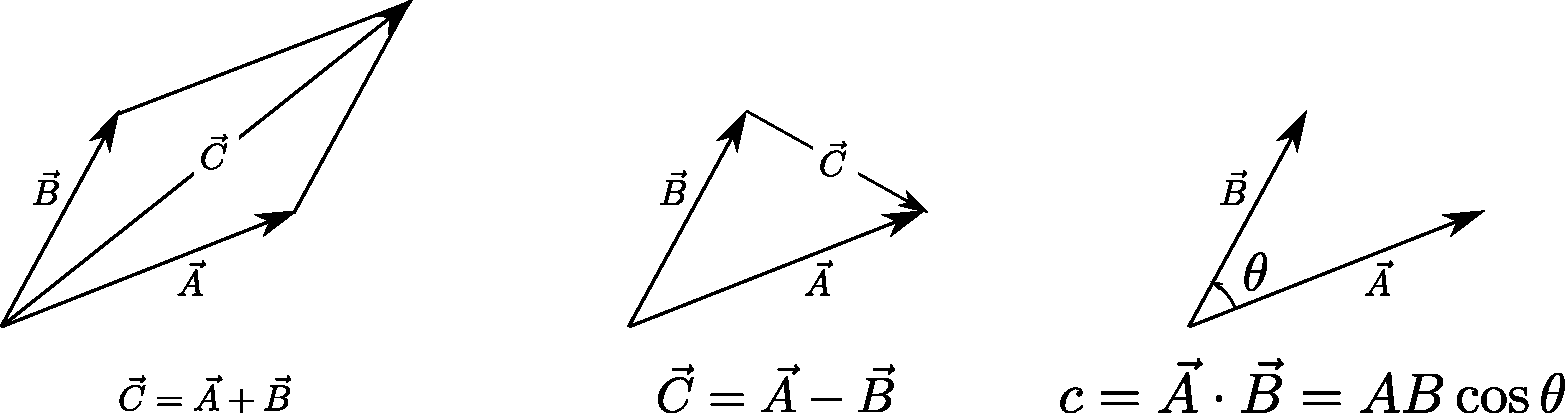
\includegraphics[width=0.7\textwidth]{images/motion-theory-4.pdf}
\caption{矢量的三种简单运算,加减法得到新的矢量,内积得到的是一个标量}
\end{figure}

除了用图形表示矢量,还可以利用直角坐标系将矢量用它的分量表示。
当平面直角坐标系被给定了以后,如图\ref{fig: motion-矢量在坐标系中的分量}所示对于任意平面的矢量$A$,可以将它平移直到起点与坐标系的原点$O$重合,这样它在直角坐标系中可以用它的终点的坐标$(A_x,A_y)$来表示,$(A_x,A_y)$称为矢量在坐标系中的分量。
这样它与一个给定标量$c$的乘积的分量为矢量的各个分量分别与标量$c$的乘积:
\begin{equation}
(c\vec{A})_x = cA_x,\qquad (c\vec{A})_y = cA_y
\end{equation}
同样对于另外一个矢量$\vec{B} = (B_x, B_y)$,它与$\vec{A}$的加法、减法以及内积的分量则可分别表示为
\begin{align}
&(A+B)_x = A_x+B_x, \qquad (A+B)_y = A_y+B_y&\\
&(A-B)_x = A_x-B_x, \qquad (A-B)_y = A_y-B_y&\\
&A\cdot B = A_x\cdot B_x+A_y\cdot B_y&
\end{align}
\begin{figure}[hbtp]
\centering
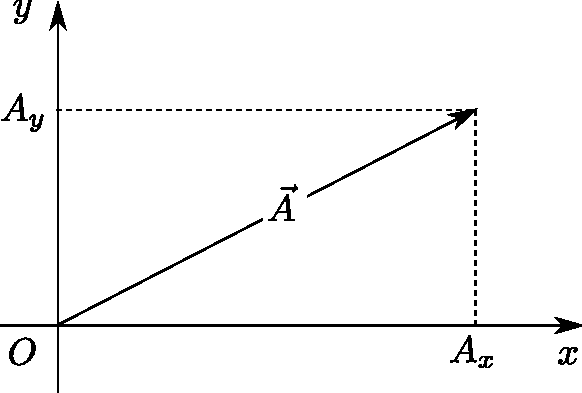
\includegraphics[width=0.4\textwidth]{images/motion-theory-5.pdf}
\caption{矢量的分量,将矢量平移到原点,其终点的坐标即矢量的分量值}\label{fig: motion-矢量在坐标系中的分量}
\end{figure}

\begin{example}
对一个运动质点的观测表明在$t_1$时刻位于$A$点,$t_2$时刻位于$B$点,$t_3$时刻位于$C$点,分别在图中给出它在$t_1\rightarrow t_2$,$t_2\rightarrow t_3$时间段中的位移,$t_1\rightarrow t_3$的位移。
从中你能够得到什么结论?
\tagged{student}{\vspace*{4cm}}
\begin{taggedblock}{teacher}
\newline
解析:略
\vspace*{5cm}
\end{taggedblock}
\end{example}

\begin{example}
已知一个运动质点在$t_1\rightarrow t_2$的位移为$\vec{D}_1$,$t_1\rightarrow t_3$的位移为$\vec{D}_2$,求它在$t_2$到$t_3$时间内的位移。
\tagged{student}{\vspace*{4cm}}
\begin{taggedblock}{teacher}
\newline
解析:略
\vspace*{4cm}
\end{taggedblock}
\end{example}

\begin{example}
为了描写一个在给平面上质点的运动,建立平面直角坐标系。
$t=0$时质点的坐标为$(2,3)$,随后运动过程产生的位移由矢量$(4,5)$给出,所有量的单位都是米,求最终质点所处的位置。
\tagged{student}{\vspace*{4cm}}
\begin{taggedblock}{teacher}
\newline
解析:根据位移的关系以及矢量在坐标系中的运算法则可知最终的位置
\[(x,y) = (2,3)+(4,5) = (6,8).\]
\end{taggedblock}
\end{example}




\subsection{运动的快慢:速度}
运动质点的{\heiti 速度}被定义为位移随时间的变化率,所以它和位移一样不但有大小而且有方向。
对于一个在$t$时刻位于$\vec{r}(t)$而在$\dt$时刻位于$\vec{r}(t+\dt)$运动的质点来说它的平均速度的定义为
\begin{equation}
\vec{v} = \frac{\vec{r}(t+\dt)-\vec{r}(t)}{\dt}=\frac{\Delta \vec{r}}{\Delta t}.
\end{equation}
当$\dt$很小时可以发现速度的方向和此时质点运动的方向趋近于一致,其大小则等于此时的瞬时速率,称做质点的{\heiti 瞬时速度}
\begin{equation}
\vec{v}(t) = \lim_{\Delta t\rightarrow 0}\frac{\Delta \vec{r}}{\Delta t}
\end{equation}
如果物体沿曲线运动,则瞬时速度的方向实际上就是轨迹切线的方向。


\begin{figure}[hbtp]
\centering
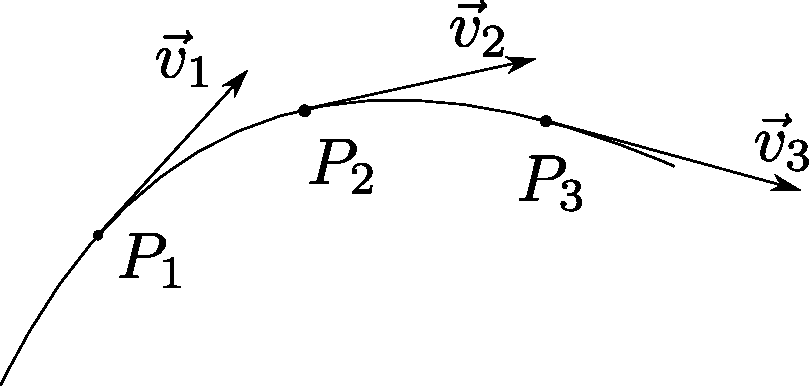
\includegraphics[width=0.5\textwidth]{images/motion-theory-6.pdf}
\caption{曲线运动轨迹上各点的瞬时速度,大小等于瞬时速率,方向沿着曲线切线的方向}\label{fig: motion-曲线上各点的瞬时速度}
\end{figure}


当一个物体在某一时刻的位置$\vec{r}$和速度$\vec{v}$同时为已知时,则在一微小时刻$\dt$之后它所处的位置由
\begin{equation}
\vec{r}(t+\dt) = \vec{r}+\vec{v}\dt
\end{equation}
所给出。
如果质点的运动速度的大小和方向都不随时间而变化时,这样的运动被称为{\heiti 匀速直线运动}。
当一个做匀速直线运动的质点在$t=0$时的位置为$\vec{r}_0$,而它的速度为$\vec{v}$时,非常容易地,在任意$t$时刻它的位置为
\begin{equation}
\vec{r}(t) = \vec{r}_0+\vec{v}t.
\end{equation}





\begin{example}
飞机由机场起飞后以速度$v=800\unit{km/h}$沿北偏东$53^\circ$的方向行驶了1小时间以后突然接到紧急命令需要在半小时内到达位于出发机场正东1000 km的机场$B$,求调整航向以后的速度的大小和方向。
可取近似值$\sin53^\circ = \frac{4}{5}$
\tagged{student}{\vspace*{3cm}}
\begin{taggedblock}{teacher}
\newline
解析:设1小时后飞机到达$C$点,通过位置关系可以判断出$B$在$C$的南偏东$37^\circ$方向$600\unit{km}$处,这样如果飞机在给定的时间内到达,它的的速度大小必须为$1200\unit{km/h}$,方向指向前面给出的方向。
\end{taggedblock}
\end{example}



\begin{example}
如图所示,有一艘潜艇潜伏于$A$点,一艘敌船以匀速$v$沿直线$MN$航行,$A$点到$MN$的垂线距离为$L$。
潜艇发射的鱼雷速度为$u$,沿直线匀速运行,在不被发现的情况下当敌船航行到图中所示的$\theta$角时发射可使鱼雷垂直击中,造成最大的破坏,求$\theta$角的大小与已知物理量的关系。

\begin{flushright}
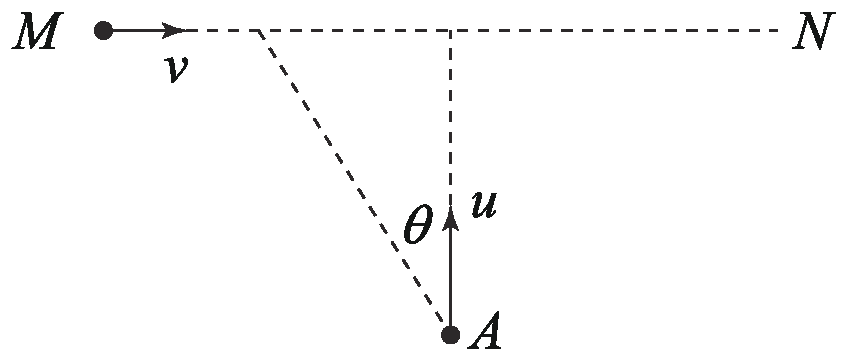
\includegraphics[width = 0.5\textwidth]{images/motion-30.pdf} 
\end{flushright}
\tagged{student}{\vspace*{4cm}}
\begin{taggedblock}{teacher}
\noindent
解析:做出船和鱼雷满足条件的运行轨迹,解三角形可知
\[
\tan\theta = \frac{vt}{ut} = \frac{v}{u},
\]
可见发射角度与它们之间的距离无关,只与速度有关。
\vspace*{3cm}
\end{taggedblock}
\end{example}

\begin{example}
足球比赛,一攻方队员在图中的$A$处沿$AX$方向传球,球在草地上以速度$v$匀速滚动,守方有一队员在图中$B$处,以$d$表示$A$、$B$间的距离,以$\theta$表示$AB$与$AX$之间的夹角,已知$\theta <90^\circ$,设在球离开A处的同时,位于B处的守方队员开始沿一直线在匀速运动中去抢球,以$v_p$表示他的速率,在不考虑场地边界限制的条件下,求出守方队员可以抢到球的必要条件。

%2.如果攻方有一接球队员个处在$AX$线上等球,以$r$表示他到$A$点的距离,求球不被原在$B$处的守方队员抢断的条件。
%
%3.如果攻方有一接球队员个处在$AX$线上等球,以$r$表示他到$A$点的距离,在球离开$A$处的同时,他开始匀速跑动去接球,以$v_r$表示其速率,求在这种情况下球不被原在$B$处的守方队员抢断的条件。
\begin{flushright}
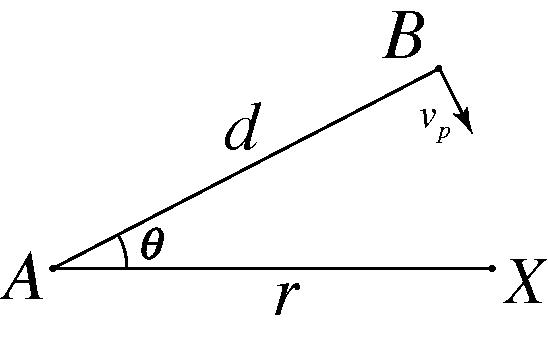
\includegraphics[width = 0.3\textwidth]{images/motion-problem-football.pdf}
\end{flushright}
\tagged{student}{\vspace*{4cm}}
\begin{taggedblock}{teacher}
\vspace*{4cm}
\noindent
解析:如上图所示,球员能够抢到球说明在某一时刻他和球处于同一位置,假设时间为$t$,这时球员跑过的距离为$v_pt$,球跑过的距离为$vt$,三角形中根据余弦定理我们有
\[
v_p^2t^2 = d^2+v^2t^2-2vtd\cos\theta,
\]
这是一个关于时间的一元二次方程
\[
(v_p^2-v^2)t^2+2dv\cos\theta t-d^2=0.
\]
能够抢到球说明这个方程有解,也就是它的判别式大于等于零:
\[
\Delta  = 4d^2v^2\cos^2\theta+4d^2(v_p^2-v^2)\ge 0,\text{可得},\qquad v_p\ge v\sin\theta.
\]
\end{taggedblock}
\end{example}

\begin{example}
两个质点$A$、$B$同时从$P$、$Q$两点出发,分别以速度$\vec{v}_{1}$沿直线$AB$和以速度$\vec{v}_2$沿PR作匀速直线运动,$QR$和$QP$的夹角为$\alpha$,开始时$PQ$两点相距$l$,求此后两质点的最短距离。
\begin{flushright}
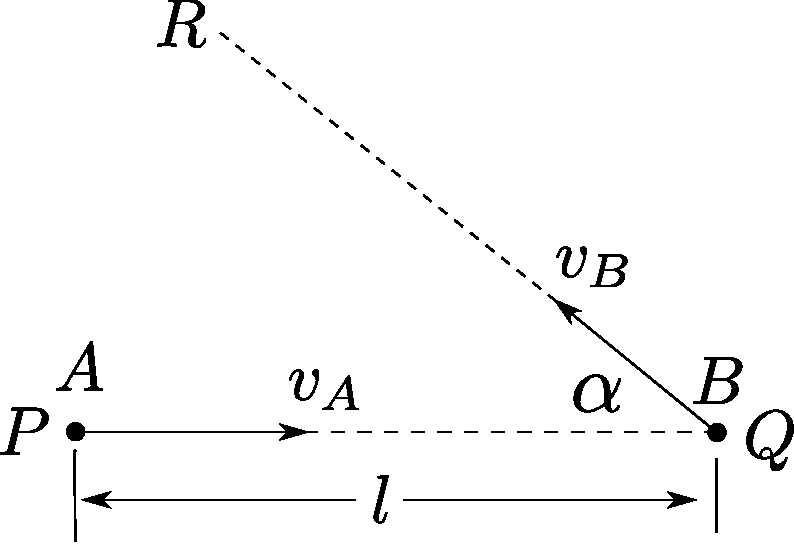
\includegraphics[width = 0.3\textwidth]{images/motion-problem-29.pdf}  
\end{flushright}
\tagged{student}{\vspace*{4cm}}
\begin{taggedblock}{teacher}
\noindent
解析:建立一个原点在$A$点,$x$轴沿两点连线方向的坐标系,两个质点的运动可以用它们的坐标来表示,分别为
\[x_A = v_At,\qquad y_A = 0\]
\[x_B = l-v_B t\cos\alpha,\qquad y_B = v_Bt\sin\alpha.\]
这样根据勾股定理两点之间距离的平方可以表示为
\begin{eqnarray*}
d^2& =& (x_A-x_B)^2+(y_A-y_B)^2 = [l-(v_B\cos\alpha+v_A)t]^2+[v_Bt\sin\alpha]^2\\
&=& (v_B^2+v_A^2+2v_Av_B\cos\alpha)t^2-2(v_B\cos\alpha+v_A)lt+l^2
\end{eqnarray*}
是一个关于$t$的二次函数,根据二次函数图像的性质可知其对称轴位于
\[
t = \frac{v_B\cos\alpha+v_A}{v_B^2+v_A^2+2v_Av_B\cos\alpha}l
\]
处,这时它们之间的距离可将上面的时间代入距离的表达式中得到:
\[
d_{min}^2 = \left[1-\frac{(v_B\cos\alpha+v_A)^2}{v_B^2+v_A^2+2v_Av_B\cos\alpha}\right]l^2,\qquad d_{min} = \frac{v_B\sin\alpha}{\sqrt{v_B^2+v_A^2+2v_Av_B\cos\alpha}}l
\]


\end{taggedblock}
\end{example}


\begin{example}
如图所示,一个人在图中$A$点处看到一个人在水中$B$点求救,已知它在地面奔跑的速度为$v_1$,在水中游泳的速度为$v_2$,各个长度已在图中标出。
求他能够在最短时间到达落水点$B$所走的路径。
\begin{flushright}
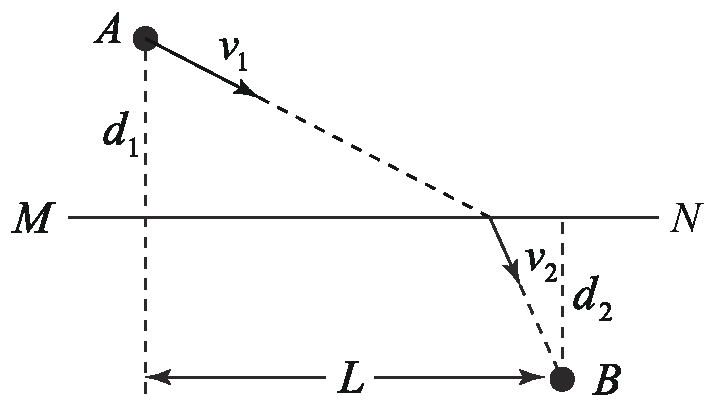
\includegraphics[width = 0.4\textwidth]{images/motion-31.pdf} 
\end{flushright}
\tagged{student}{\vspace*{3cm}}
\begin{taggedblock}{teacher}
\vspace*{2cm}
\noindent
解析:类比光的折射定律,可以得到
\[
\frac{1}{v_1}\sin\theta_1 = \frac{1}{v_2}\sin\theta_2
\]
\end{taggedblock}
\end{example}

\subsection{速度的变化:加速度}
\begin{figure}[hbtp]
\centering
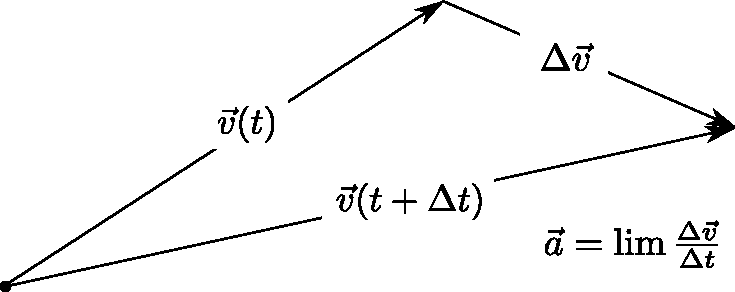
\includegraphics[width=0.6\textwidth]{images/motion-theory-7.pdf}
\caption{质点运动过程中速度的变化,加速度}
\end{figure}

和一维的情况类似,平均加速度被定义为给定时间$\dt$里速度的变化率
\begin{equation}
\vec{a} = \frac{\vec{v}(t+\dt)}{\dt}=\frac{\Delta \vec{v}}{\dt},
\end{equation}
而上式在$\Delta t\rightarrow 0$的极限情况下的值为质点在$t$时刻的瞬时加速度:
\begin{equation}
\vec{a}(t) = \lim_{\Delta t\rightarrow 0}\frac{\Delta\vec{v}}{\Delta t}
\end{equation}
和速度和位移一样,一般情况下的加速度也是一个矢量,大小为速度变化量随时间的变化率,而方向给出了速度变化的方式。
因为速度是一个矢量,当它的大小或者方向发生变化时都会带来非零的加速度。




当质点在某一时刻$t$时的速度$\vec{v}(t)$和此时它的加速度$\vec{a}$同时为已知时,在此后$\dt$时间后它的速度为
\begin{equation}
\vec{v}(t+\dt) = \vec{v}(t)+\vec{a}\dt.
\end{equation}
加速度的大小和方向都不变的运动被称为{\heiti 匀加速运动}。
$t=0$时位于$\vec{r}_0$,速度为$\vec{v}_0$的做加速度为$a$的匀加速运动速度和位置随时间的变化率形式相对简单:
\begin{eqnarray}
\vec{v}(t) &=& \vec{v}_0+\vec{a}t\\
\vec{r}(r)&=&\vec{r}_0+\vec{v}_0t+\frac{1}{2}\vec{a}t^2
\end{eqnarray}



\section{抛体运动}
在地球表面附近抛出的物体在阻力可以忽略不计时的运动称之为抛体运动。
观测表明抛体运动是均加速运动,运动过程中加速度的大小等于重力加速度$g$,方向指向地面。
当初始速度的方向与地表的垂线方向一致,也就是竖直向上或向下时,抛出的质点将作直线运动,但如果初始速度有水平方向的分量时,运动的轨迹将是一条曲线,曲线的形状和大小与初速度的大小和方向密切相关,数学上将这类曲线统称为{\heiti 抛物线}
因为抛体的运动易于观察,所以我们首先集中精力研究抛体运动的一般性质和处理方法,在这里所学的方法和结果实际上能够很轻易地推广到其它的的匀加速运动中去。

在不考虑复杂因素的理想情形下,斜向抛出的物体将在一个平面内运动。
为了方便地研究抛体的运动,我们在它运动的平面内建立一个平面直角坐标系,简单起见,设坐标系的原点与抛体运动的起始点重合,$x$轴与初速度的水平分量的方向一致,称为水平方向,$y$轴垂直于地面竖直向上,称之为竖直方向。
在这样的坐标系原点处抛出质点的速度大小为$v_0$,它与水平方向的夹角定义为$\theta$,这样的两个量唯一地决定了抛体此后的运动状态。
为了定量地描写抛体的运动,我们用它在运动过程中某一时刻$t$的水平和竖直坐标值来表示它的位置。
抛体运动过程中水平和竖直方向的运动行为不同,它的水平坐标值$x$随着时间的推移均匀地增大,看上去像是在作匀速直线运动,其匀速运动的速度就是初始速度的水平分量:
\begin{eqnarray}
v_x(t)& =& v_0\cos\theta\label{eqn: motion-抛体的水平速度}\\
x(t) &=& v_0\cos\theta\cdot  t\label{eqn: motion-抛体的水平运动}
\end{eqnarray}

而在竖直坐标$y$随时间的变化关系则和以初速度的竖直分量$v_{y0} = v\sin\theta$为初速度的竖起上抛运动完全一致:
\begin{eqnarray}
v_y(t)& =& v_0\sin\theta\cdot  t-gt\label{eqn: motion-抛体的竖直速度}\\
y(t) &=& v_0\sin\theta\cdot t-\frac{1}{2}gt^2\label{eqn: motion-抛体的竖直运动}
\end{eqnarray}

像上面那样把一个空间中的曲线运动用它在某一坐标系中的各个坐标值随时间的关系来表示的过程称之为{\heiti 运动的分解},反过来如果知道了一个特定的运动过程在某一坐标系中的各个坐标随时间的关系,那么它在空间中的运动行为就被唯一地决定,这样的处理过程称为{\heiti 运动的合成}。
将一个复杂的运动首先分解为沿着各个方向的分运动,在搞清楚各个方向的分量运动的行为之后再将它们统一起来得到最终的运动是运动学中非常常用的方法。
以前面抛体运动为例,看上去抛体的运动是具有一定的复杂性的曲线运动,但将它的运动过程用它的水平和竖直坐标来描写时发现它们都满足简单的运动规律,水平方向上作匀速直线运动,而在竖直方向上稍复杂一些,也不过是竖直的落体运动。


水平和竖直方向的分运动合起来就是完整的抛体运动。
抛出物体的运动轨迹可由它们的运动方程\ref{eqn: motion-抛体的水平运动},\ref{eqn: motion-抛体的竖直运动}导出,从\ref{eqn: motion-抛体的水平运动}中解出时间
\[
t = \frac{x}{v_0\cos\theta}
\]
将它代入\ref{eqn: motion-抛体的竖直运动}当中就是可消去时间$t$从而得到抛体运动过程中任何一点处的竖直坐标和此时物体水平坐标的关系,也就是抛体的{\heiti 轨迹方程}
\begin{equation}\label{eqn: motion-抛体的轨迹方程}
y(x) = \tan\theta\cdot x-\frac{g}{2v_0^2\cos^2\theta}x^2
\end{equation}
可以看出上式当中$y$是水平坐标$x$的二次方程,这就是数学上将二次方程代表的曲线称为抛物线的原因。
进一步观察上式还可以看出所有的抛体轨迹在我们选取的坐标系中都是开口向下的抛物线,其对称轴的位置和宽度由初始条件,也就是初速度的大小$v_0$和角度$\theta$共同决定。
当初速度和抛射角取一些特殊值时的,一般的抛体运动退化成相对简单的运动形式,例如
\begin{itemize}
\item
自由落体运动:$v_0 = 0$
\item
竖直上抛运动:$v_0>0$,$\theta =  \frac{ \pi}{2}$
\item
竖直下抛运动:$v_0>0$, $ \theta = - \frac{ \pi}{2}$
\item
平抛运动: $v_0>0$, $ \theta=0$
\end{itemize}
以上就是抛体运动所满足的所有规律,灵活地使用这些基本的关系式就可以解决几乎所有和抛体运动有关的问题,以下是一些例子:

\begin{example}
网球的规则要求发球时球不能碰到球网,并且落到对方场地的指定区域(发球区)。
将发球过程简化为如下模型,整个网球场的长度为$2L$,发球区距离球网的距离为$l$,球网的高度为$h$,将球员发出球的运动简化为由高度$H$处以初速度$v_0$的平抛运动。
请证明击球的高度$H$必需大于某一给定值$H_0$才能够在规则允许的条件下将球发出,并求出$H_0$与其它已知量的关系。
\begin{flushright}
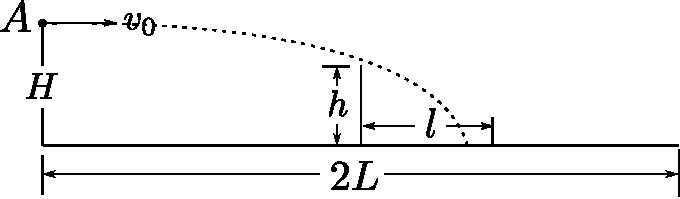
\includegraphics[width = 0.5\textwidth]{images/motion-8.pdf}
\end{flushright}
\tagged{student}{\vspace*{3cm}}
\begin{taggedblock}{teacher}
\noindent
解析:建立一个以一方端线为原点的坐标系,$x$轴指向对方场地,$y$轴指向上。
以初速度$v_0$抛出的物体的运动轨迹方程为
\[
y = H -\frac{gx^2}{2v_0^2}
\]
不碰到球网要求$x=L$时$y>h$:
\[
H-\frac{gL^2}{2v_0^2}>h,\qquad v_0^2>\frac{gL^2}{2(H-h)}
\]
而发球不出发球区则要求$x=L+l$时$y<0$:
\[
H-\frac{g(L+l)^2}{2v_0^2}<0,\qquad v_0^2<\frac{g(L+l)^2}{2H},
\]
这样联立以上两式可以看到要想满足条件需要
\[
\frac{gL^2}{2(H-h)}<\frac{g(L+l)^2}{2H},\qquad\textbf{解得}\qquad H>h\frac{(L+l)^2}{2Ll+l^2}
\]
\end{taggedblock}
\end{example}

%%%%%%%%%%%%%%%%%%%%%%%%%%%%%%%%%%
\begin{example}
将一块石头从$20\unit{m}$高的山顶上水平抛出,当石块落到地面上时,其速度方向与水平面成$45^\circ$角。
请问石块抛出时的速度是多少?
\begin{flushright}
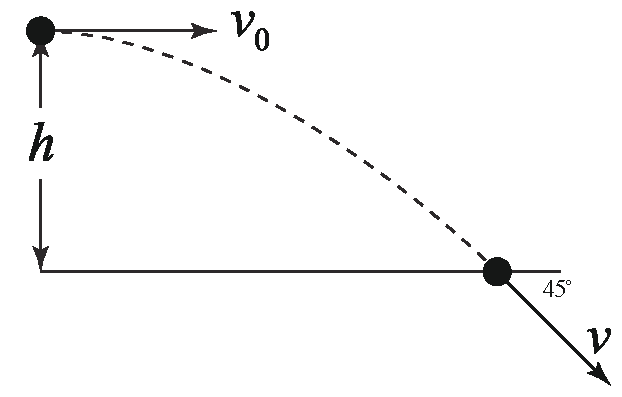
\includegraphics[width = 0.4\textwidth]{images/motion-32.pdf} 
\end{flushright}
\tagged{student}{\vspace*{2cm}}
\begin{taggedblock}{teacher}
\noindent
解析:通过抛体运动的分解可知落地时竖直方向的速度
\[
v_y = \sqrt{2gH} = 20\unit{m/s}
\]
而在运动过程中水平方向速度不变,所以如果最后以45度角撞向地面则要求水平速度$v_x = v_y = 20\unit{m/s} $。
\end{taggedblock}
\end{example}


\begin{example}
作斜上抛质点的射程被定义为当它再次落到与抛出点相同高度时的水平距离,试证明由初速度$v_0$、仰角$\theta$抛出物体的射程$S$满足
\[ S = \frac{v_0^2}{g}\sin 2\theta \]
并以此证明对于相同的初始速率$v_0$以斜向上$45^\circ$角抛出的物体射程最大。
\begin{flushright}
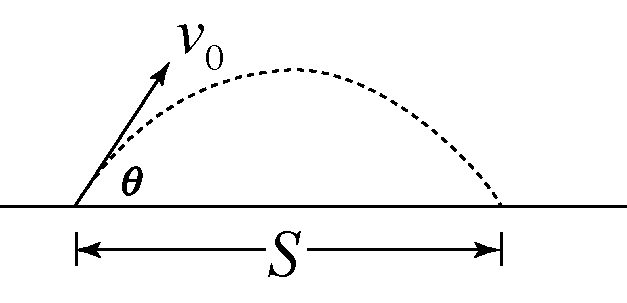
\includegraphics[width=0.4\textwidth]{images/motion-problem-2.pdf}
\end{flushright}
\tagged{student}{\vspace*{3cm}}
\begin{taggedblock}{teacher}
\noindent
解析:再次落到相同高度的时间由方程
\[
v_0\sin\theta t-\frac{1}{2}gt^2=0,\qquad t = \frac{2v_0\sin\theta}{g}
\]
给出,在这样的时间里水平方向的运动距离
\[
x = v_0\cos\theta t = v_0\cos\theta  \frac{2v_0\sin\theta}{g} = \frac{2v_0^2}{g}\sin\theta\cos\theta = \frac{v_0^2}{g}\sin 2\theta
\]
得证!
根据三角函数的性质可知,当$\theta = \frac{\pi}{4}$时上面的正弦取最大值,也就是射程达到最大,并且从中还可知最大射程
\[
S_{max} = \frac{v_0^2}{g}
\]
\end{taggedblock}
\end{example}

\begin{example}
一个以给定的初速度$v_0$,仰角为$\theta_1$抛出的物体的射程为$S$,求证以同样的初速度,仰角$\theta_2 = \pi/2-\theta_1$抛出物体的射程也是$S$,且射程相同的两个抛体在空中停留的时间乘积$t_1t_2 = \frac{2S}{g}$
\begin{flushright}
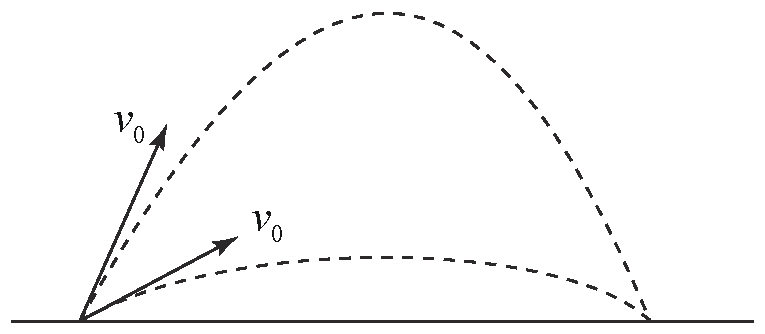
\includegraphics[width = 0.4\textwidth]{images/motion-33.pdf} 
\end{flushright}
\tagged{student}{\vspace*{4cm}}
\begin{taggedblock}{teacher}
\noindent
解析:根据前面一问得到的结果,射程和角度以及初速度大小的关系为$S = \frac{v_0^2}{g}\sin 2\theta$,相同初速率抛出的物体要想射程相同,需要有
\[
\sin 2\theta_1 = \sin 2\theta_2,\qquad \theta_1+\theta_2 = \frac{\pi}{2}.
\]
它们在空中飞行的时间分别为
\[
t_1 = \frac{2v_0\sin\theta_1}{g},\qquad t_2 = \frac{2v_0\sin\theta_2}{g}
\]
这样将它们相乘可得
\[t_1t_2 = \frac{4v_0^2}{g^2}\sin\theta_1\sin\theta_2 = \frac{2v_0^2}{g^2}\sin 2\theta_1 = \frac{2S}{g}\]
\end{taggedblock}
\end{example}



%
%\begin{example}
%求给定点$A$以相同大小的初始速率$v_0$沿不同仰角抛出的所有物体当中,当它的水平位置到达与抛出点相距$L$时可能的最大高度,以及能够到达该高度的仰角值。
%\begin{flushright}
%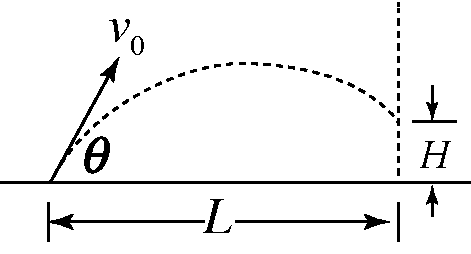
\includegraphics[width=0.3\textwidth]{images/motion-problem-3.pdf}
%\end{flushright}
%\tagged{student}{\vspace*{4cm}}
%\begin{taggedblock}{teacher}
%\noindent
%解析:
%\end{taggedblock}
%\end{example}



\begin{example}
求从图中$A$点抛出的物体能够越过距离$A$点$L$处的一个高度为$H$的障碍物所需要的最小速度。
\begin{flushright}
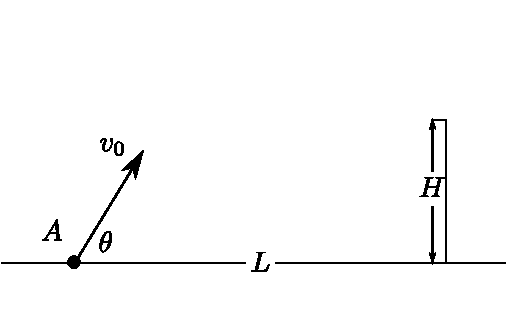
\includegraphics[width=0.34\textwidth]{images/motion-9.pdf} 
\end{flushright}
\tagged{student}{\vspace*{3cm}}
\begin{taggedblock}{teacher}
\noindent
解析:建立标准的坐标系,抛体的轨迹由方程\ref{eqn: motion-抛体的轨迹方程}给出。
根据题目的要求,需要它在运动到$x=L$时的高度至少为$H$,简单的分析可知最小的速度一定会出现在$y=H$时,根据三角函数的性质上面的条件等价于当把方程
\[
H = \tan\theta L -\frac{gL^2}{2v_0^2}(1+\tan^2\theta)
\]
看做是$\tan\theta$的一元二次方程时有解。
这个要求等价于方程的判别式
\[
\Delta  = L^2 - 4\frac{gL^2}{2v_0^2}(H+\frac{gL^2}{2v_0^2})\geq 0
\]
判别式在$v_0$很大时必然会小于零,而第一次出现等于零的值就意味着最小初速率,它等于零的解经过代数计算可得
\[
v_0^2 = \frac{gL^2}{\sqrt{L^2+H^2}-H}
\]
这个速度就是能够打过障碍的最小速度。
\end{taggedblock}
\end{example}


\begin{example}
对于一个从给定点$A$以给定的速率$v_0$不同角度抛出的物体来说,它所有可能到达的区域和不可能到达的区域有一条分界线,求该分解线在如图所示的坐标系中的方程。
\begin{flushright}
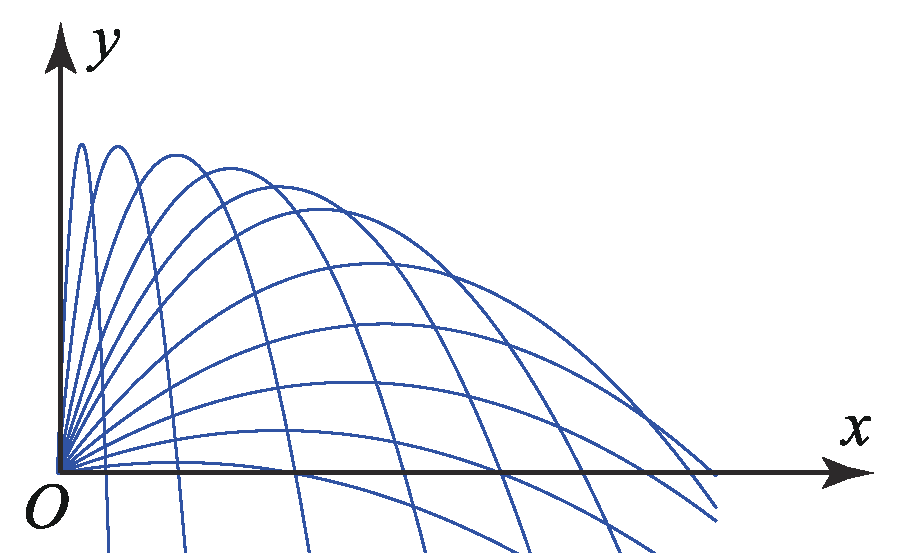
\includegraphics[width = 0.4\textwidth]{images/motion-34.pdf} 
\end{flushright}
\tagged{student}{\vspace*{4cm}}
\begin{taggedblock}{teacher}
\noindent
解析:原点抛出物体的轨迹方程\ref{eqn: motion-抛体的轨迹方程}为已知,这样对于给定的水平位置$x$处,以相同的初速率但角度不同的抛出物体当中,所能够达到的最大高度由
\[
\tan\theta = \frac{v_0^2}{gx}
\]
所给出的抛射角度给出,将这个抛射角度代入到轨迹方程中可得在给定$x$处最大高度
\[
y_max = -\frac{g}{2v_0^2}x^2+\frac{v_0^2}{2g}
\]
这就是所求的曲线方程。
\end{taggedblock}
\end{example}


\begin{example}
铅球运动员能够推出铅球的最大速度为$v_0$,肩膀距离地面的高度为$H$,求它能够推出最好成绩时铅球出手的速度方向与地面的夹角。
当$v_0 = 12.37 \unit{m/s}$,$H = 1.5\unit{m}$时求出能够得到最好成绩时的角度值以及他所获得的成绩。
\tagged{student}{\vspace*{4cm}}
\begin{taggedblock}{teacher}
\newline
解析:在初速度和高度差为已知时,想知道在给定的高度差下铅球所能够到达的最远距离,也就是上一问当中求出的曲线中$y=-H$所对应的水平坐标$x$:
\[
x = \sqrt{\frac{v_0^4}{g^2}+\frac{2v_0^2H}{g}}\simeq 23.12\unit{m}
\]
\end{taggedblock}
\end{example}

\begin{example}
在小丘上置一靶子,在炮位所在处看靶子的仰角为$\alpha$,炮与靶子间的水平距离为$L$,向目标射击时炮身的仰角为$\beta$,炮弹以什么初速度发射才能击中目标。
\begin{flushright}
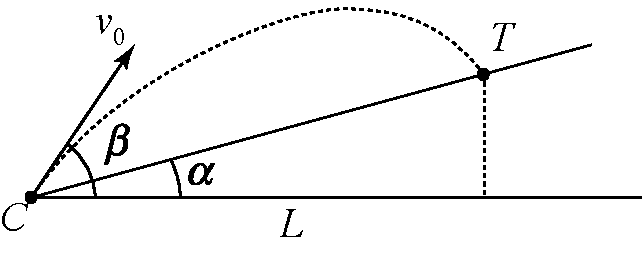
\includegraphics[width = 0.4\textwidth]{images/motion-problem-31.pdf} 
\end{flushright}
\tagged{student}{\vspace*{4cm}}
\begin{taggedblock}{teacher}
\noindent
解析:设速率为$v$则能够击中目标所需要满足的条件为
\[
L\sin\alpha = L\cos\alpha\tan\beta-\frac{gL^2\cos^2\alpha}{2v^2\cos^2\beta},
\]
解出上述方程即可得初速度
\[
v=\sqrt{\frac{gL\cos^2\alpha}{2\cos^2\beta(\cos\alpha\tan\beta-\sin\alpha)}}
\]
\end{taggedblock}
\end{example}



除了使用由方程\ref{eqn: motion-抛体的水平速度}-\ref{eqn: motion-抛体的轨迹方程}给出的代数方程以外,在解决有些问题时使用几何方法会极大降低计算量,并突出物理意义。
因为抛体运动就是匀加速度运动,在给定的时间$t$里速度的变化量就是重力加速度$g$乘以时间$t$,不要忘了速度是一个矢量,所以速度的改变量大小为$gt$,而方向指向地面。
当抛体的初始速度矢量$\vec{v}_0$被给定了以后,任一时刻$t$的速度矢量由
\begin{equation}
\vec{v}(t)=\vec{v}_0+\vec{g}t
\end{equation}
或者由图\ref{fig: motion-矢量抛体运动描写}(a)所给出的几何图形给出。
同样的道理从抛出点算起,抛体任一时刻的位移则可以用矢量表达为
\begin{equation}
\vec{r}(t)=\vec{v}_0t-\frac{1}{2}\vec{g}t^2
\end{equation}
其图形化的表示由图\ref{fig: motion-矢量抛体运动描写}(b)表示。
从中可以看出抛体的运动过程中任何时刻的位移可以看成是以初速度$\vec{v}_0$的匀速直线运动和一个自由落体运动的合成,这个图像可以极大地方便我们分析抛体的运动。
从两个图中还可以看到,当把代表位移的矢量关系图中代表自由落体的矢量放大一倍以后再与起始点连接构成的图形和代表速度矢量关系的图形相似。
\begin{figure}[hbtp]
\centering
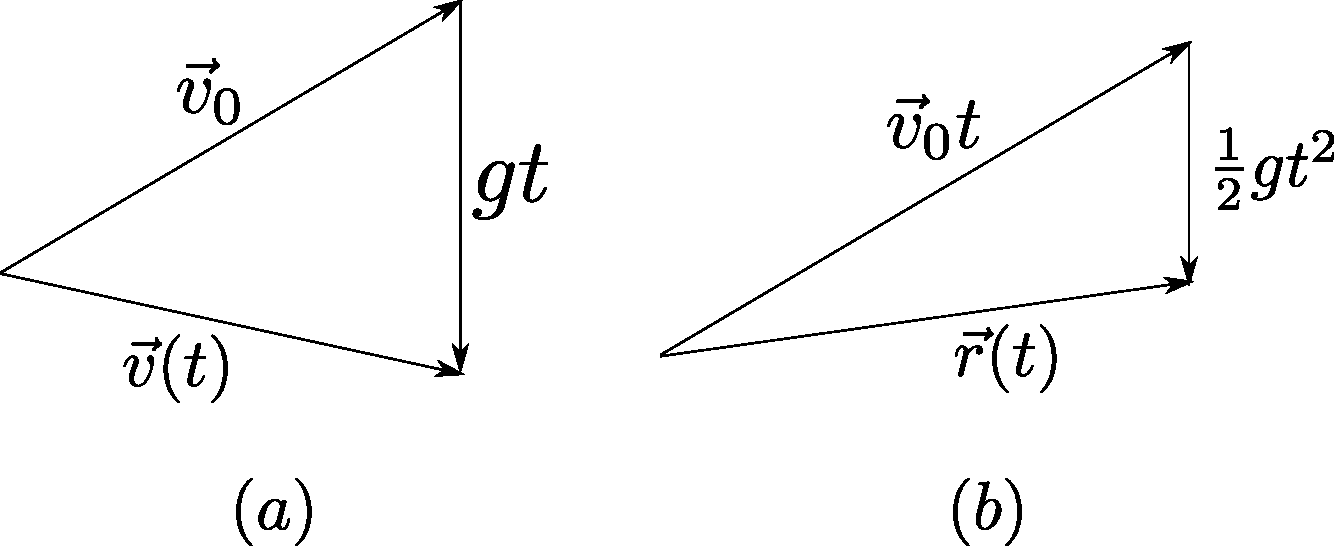
\includegraphics[width = 0.6\textwidth]{images/motion-10.pdf}
\caption{用矢量来表示抛体运动过程中任一时刻的速度和位移,如果两个图形代表的是同一个运动过程的话,这时它处于下降阶段但依然没有回落到与抛出点相同的高度}\label{fig: motion-矢量抛体运动描写}
\end{figure}

\begin{example}
在水平地面上距离$A$点距离为$L$处有一个高为$H$的障碍物,若从$A$点抛出的物体正好通过障碍物上端时的速度方向平行于地面,求抛出的仰角$\theta$和初始速率$v_0$。
\begin{flushright}
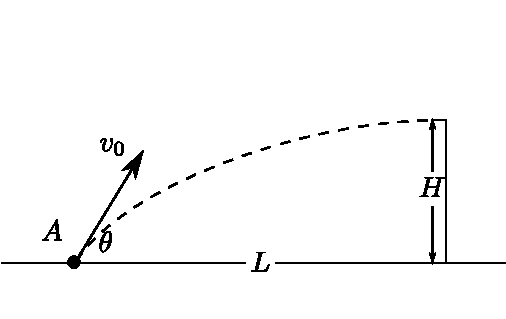
\includegraphics[width=0.3\textwidth]{images/motion-11.pdf} 
\tagged{teacher}{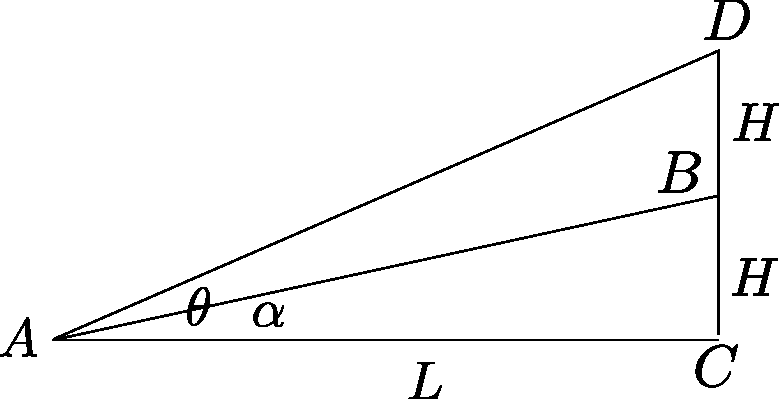
\includegraphics[width = 0.4\textwidth]{images/motion-solution-tt.pdf} }
\end{flushright}

\tagged{student}{\vspace*{3cm}}
\begin{taggedblock}{teacher}
\noindent
解析:用代数的方法当然能够求解,但是如果用几何的方法则特别地简单。
如上图所示,AC代表平面距离,BC代表墙,角DAC就是抛出时速度与地面的夹角$\theta$。
代表质点位置变化的矢量关系由三角形ADB给出,而代表速度变化的矢量关系则由三角形ACD给出。
这样的图形能够满足题目所给出的条件,刚好通过顶部并且速度与地面平行。
根据要求,BA与AC的夹角需要等于墙的顶部与抛出点连线与水平面的夹角$\tan\alpha = \frac{H}{L}$,而且DB=CB由位移和速度图形的相似关系。
这样抛出速度与地面的夹角必须满足
\[
\tan\theta = \frac{2H}{L}
\]

\end{taggedblock}
\end{example}


\begin{example}
在一个与地面夹角为$\alpha$的斜面底部斜向上抛出一个物体,当它的仰角为何值时在击中斜面时速度方向刚好与斜面垂直?
\begin{flushright}
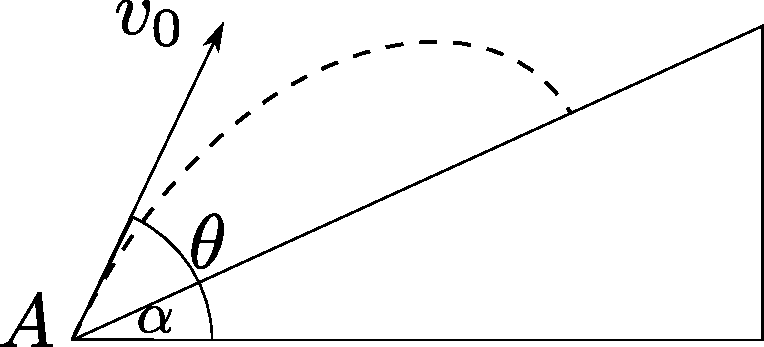
\includegraphics[width = 0.3\textwidth]{images/motion-12.pdf} 
\tagged{teacher}{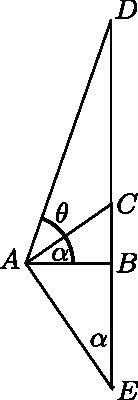
\includegraphics[height=1.5in]{images/motion-solution-12.pdf} }
\end{flushright}
\tagged{student}{\vspace*{4cm}}
\begin{taggedblock}{teacher}
\noindent
解析:如右图所示,假设三角形ADC代表表示位移的矢量关系,简单的分析可知当把DC边向下延长一倍以后的三角形与表示速度的三角形相似。
根据题目中的要求,需要角$AEB = \alpha$才能够垂直击中斜面,角$CAB = \alpha$才能够刚好落到斜面上,两个条件同时满足就可以满足前面的要求。
根据几何关系角$CAE$就是直角,并且$DC=CE$,这时图中的角$BAD$就是所需要的抛出仰角。
设$AC=L$,这样
\[
\tan\theta  = \frac{DC+CB}{AB} = \frac{\frac{L}{\sin\alpha}+L\sin\alpha}{L\cos\alpha} = \frac{\frac{1}{\sin\alpha}+\sin\alpha}{\cos\alpha}
\]
就得到了角度$\theta$与斜面角度$\alpha$的关系。

\end{taggedblock}
\end{example}

因为抛体的运动非常普遍,前面的几个例子并无法包含所有的情况。
当面对其它涉及到抛体运动问题时可以通过抛体运动的一般性质综合分析,最终找到问题的答案,下面就是几个例子:

\begin{example}
一个轰炸机在距离地面高度$H$处以速度$v$匀速飞行,请你设计一个描准装置,使得当飞行员在描准镜中看到目标位于十字交叉线正中时按下投弹按扭能够使炸弹准确击中目标。
如果描准镜是一个类似于望远镜的装置,求它与竖直垂线的夹角。
假设炸弹的飞行满足抛体运动规律。
\tagged{student}{\vspace*{4cm}}
\begin{taggedblock}{teacher}
\newline
解析:投出的炸弹可以看做平抛运动,它下降$H$的高度所需要的时间$t=\sqrt{\frac{2H}{g}}$,与此同时水平飞行的距离则是$vt$,这样落地点与投弹点的连线与垂线的夹角
\[
\tan\theta = \frac{vt}{H} = \frac{v\sqrt{\frac{2H}{g}}}{H} = \sqrt{\frac{2v^2}{gH}}
\]
可见与速度和高度均有关系,在投弹时需要仔细地调整描准镜才能够准确击中目标。
\end{taggedblock}
\end{example}


\begin{example}
如图所示的多级台阶,每级台阶的长度为$d$,高度为$l$,在$A$点以水平速度$v_0$抛出一个球体,球与台阶相撞以后其水平方向速度分量保持不变,但竖直方向的速度会反向,并变成碰撞前的$e$倍,$e<1$,如果球每次碰撞前与台阶相对速度均相同且其轨迹能够形成全同的往复过程,求$v_0$的大小和每次反弹以后上升的高度。
\begin{flushright}
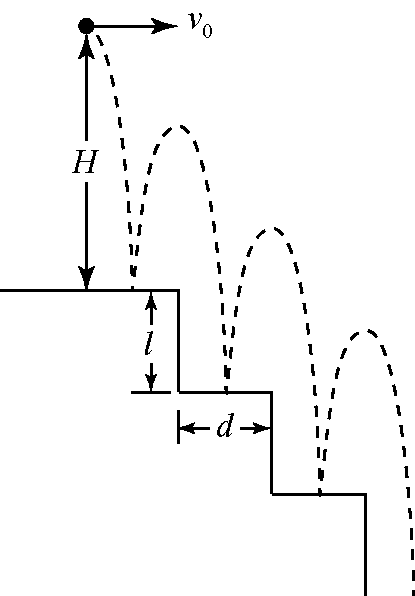
\includegraphics[width=0.3\textwidth]{images/motion-problem-30.pdf}
\end{flushright}
\tagged{student}{\vspace*{0cm}}
\begin{taggedblock}{teacher}
\noindent
解析:要想形成这样反复运动的过程,那么题目给出的量就不能是任意的,需要满足
\[
l = H(1-e^2)
\]
飞行的总时间就是每一段抛体在空中运行的时间
\[
T = (1+e)\sqrt{\frac{2H}{g}}
\]
要求在同样的时间里每次都向前飞行$d$的距离,从这个条件可知水平速度要满足
\[
v_0 = \frac{d}{T} = \frac{d}{(1+e)\sqrt{\frac{2H}{g}}}
\]
\end{taggedblock}
\end{example}



\begin{example}
一个球在距水平地面$h$高处以水平速度$\sqrt{2gh}$抛出,空气阻力不计。
小球每次落地反弹时水平速度不变,竖直速度大小按同样的比率$e$减小。
若自第一次反弹开始小球的运动轨迹与其在地面的投影之间所包围面积的总和为$\frac{8}{21}h^2$,求小球每次反弹竖直速度减小的比率$e$。

提示,小球每次做斜抛运动(从水平地面射出又落至地面)的轨迹与其在地面的投影之间所包围的面积等于其最大高度和水平射程乘积的$\frac{2}{3}$。
\tagged{student}{\vspace*{4cm}}
\begin{taggedblock}{teacher}
\newline
解析:13 年决赛第1题
\end{taggedblock}
\end{example}

\begin{example}
如图所示平面上有一个半径为$R$的球体,我们希望在地面上斜向上抛出一个物体击中球体的顶部。
求在不碰到球体的条件下能够击完成目标的最小的抛出速度$v_{min}$、抛出的角度$\theta_0$以及抛出点与球底部的距离$d_0$。
\begin{flushright}
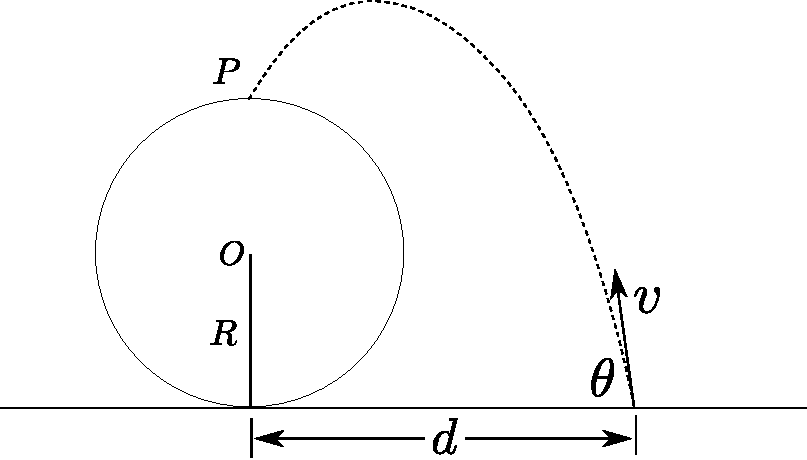
\includegraphics[width = 0.3\textwidth]{images/motion-13.pdf} 
\end{flushright}
\tagged{student}{\vspace*{4cm}}
\begin{taggedblock}{teacher}
\noindent
解析:根据抛体运动的可逆性,从地面抛出的物体如果能够击中顶部的话,以相反的速度从顶部抛出则可沿着相同的轨迹落到地面,根据能量守恒,顶部抛出物体的速度越小则到达地面时的速度就越小。
这样问题就反过来变成了从顶部抛出物体,不碰到球体表面而落到地面的最小速度。
利用前一问的答案,抛体能够打到的范围是一个随着初速度增加越来越大的抛物线,初速度不够时抛物线总会和圆有交点,这样抛体无论初速度方向如何都会碰到球。
当抛物线大到能够和球相切时就有一个可能性使沿特殊的角度抛出以后它的轨迹能够与球相切,这是不碰到球的临界条件。
当包络线与圆相切时,包络面的方程和圆的方程联立时只有一个解,当速度更大时则没有解,所以可以由这个条件解出相切对应的最小速度。
两个方程分别为
\[
y=2R+\frac{v_0^2}{2g}-\frac{g}{2v_0^2}x^2 \qquad 和\qquad
x^2+(y-R)^2=R^2
\]
注意第一个方程当中坐标系原点的变化,现在抛出点位于球的顶部,所以需要将包络线上移$2R$。
联立以后可以看做是$x^2$的一元二次方程:
\[
\frac{g^2}{4v_0^4}(x^2)^2 +\left [ 1-\frac{g}{v_0^2}(\frac{v_0^2}{2g}+R) \right ]x^2+\left [  (\frac{v_0^2}{2g}+R)^2-R^2 \right ]=0
\]
其判别式为零的条件为
\[
\Delta =(\frac{1}{2}+\frac{gR}{v_0^2})^2-4\frac{g^2}{4v_0^4}(\frac{v_0^4}{4g^2}-\frac{v_0^2R}{g})=0
\]
化简之后可以解出此时速度需要满足的条件,也就是最小的可能“击中”的速度值:
\[
v_0^2 = \frac{1}{2}gR
\]
由机械能守恒可知地面的最小抛出速度为
\[
v_{min}^2=\frac{1}{2}gR+4gR = \frac{9}{2}gR
\]
其抛出点的其它性质可由轨道给出。
\end{taggedblock}
\end{example}

\section{圆周运动}
质点沿圆的运动是另一类简单曲线运动,称为{\heiti 圆周运动}。
圆周运动是非常普遍的运动形式,在游乐场可以看到大量的圆周运动的例子,在历史上很长时间里人们一直认为天体的运动也是圆周运动。
最简单的圆周运动是质点以固定的速率沿着圆周运行,这样的运动称为{\heiti 匀速圆周运动},做匀速圆周运动的质点速度大小始终不变,但是速度的方向却在不断地变化。
根据加速度的定义可以看出即使是匀速圆周运动的质点的加速度也不为零。

最方便地描写圆周运动质点的位置并不是像研究抛体运动时的平面直角坐标系,而是用运动质点与圆心的连线与一个固定方向的夹角来表示质点的位置。
如图\ref{fig: motion-圆周运动的角位置}所示当做圆周运动的质点运动到$P$点时,它与固定方向$ON$的夹角$\theta$可以唯一地确定它在圆周上的位置$P$,我们将$\theta$称为做圆周运动质点的{\heiti 角位置},习惯上规定沿着逆时间转动的方向为$\theta$增大的方向。
从某种意义上角位置和一维运动质点的坐标有很多相似之处,但也要注意它们的不同。
例如一维运动质点的位置由其坐标唯一确定,但是角位置却不同,任意与给定的$\theta$相差$2\pi$整数倍的角度实际上给出的是同样的空间位置。
例如$\theta =0$与$\theta = 2\pi$所给出的位置都是图中的$N$点。



\begin{figure}[hbtp]
\begin{minipage}[l]{0.5\textwidth}
\centering
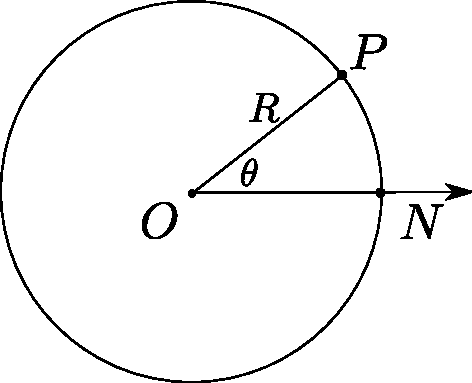
\includegraphics[height=1in]{images/motion-14.pdf}
\caption{圆周运动质点的位置用它和圆心的连线与一固定方向的夹角表示其位置}
\label{fig: motion-圆周运动的角位置}
\end{minipage} 
\begin{minipage}[r]{0.5\textwidth}
\centering
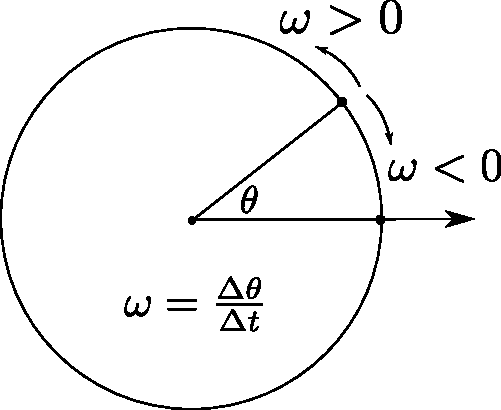
\includegraphics[height=1in]{images/motion-15.pdf} 
\caption{角速度的正负及其对应的运动方式}
\label{fig: motion-角速度的正负及其对应的运动方式}
\end{minipage}
\end{figure}


当质点在圆周上运动时,它的角位置$\theta$会随时间的推移不断地发生变化,作匀速圆周运动的质点相同时间里角位置的变化量为常数,称为匀速圆周运动的{\heiti 角速度},它定义为单位时间里角位置随时间的变化率。
如果在$\Delta t$时间里质点转过的角度为$\Delta \theta$,这时它作匀速圆周运动的角速度$\omega$就表示为
\begin{equation}
\omega = \frac{\Delta\theta}{\Delta t},
\end{equation}
从定义可以看出当质点的圆周运动方向是使$\theta$变大的方向,则角速度为正,反之角速度为负,图\ref{fig: motion-角速度的正负及其对应的运动方式}给出了实际的例子。
如果质点在圆周运动过程中角速度时刻保持不变,则称该质点作{\heiti 匀速圆周运动}。
当初始角位置和角速度均已知的匀速圆周运动,在任意时刻$t$的角位置能够表达为
\begin{equation}
\theta(t) = \theta_0+\omega t.
\end{equation}
因为角位置的周期性,在经过一段时间后它的角位置将与初始位置的差别变成$2\pi$,很容易想像实际上质点又回到了出发点。
匀速转动一周又回到起始点所需要的时间称为匀速圆周运动的{\heiti 周期},根据定义它和角速度的关系为
\begin{equation}
\omega T = 2\pi,\qquad T = \frac{2\pi}{\omega},
\end{equation}
从中可以看出角速度越大转动的周期就越短。
另外一个用来描写转动快慢的物理量为转动的{\heiti 频率},用单位时间(通常是$1\unit{s}$)内完成转动的圈数,从定义可以看出频率$f$和周期、角速度之间必然满足关系
\begin{equation}
f = \frac{1}{T} = \frac{\omega}{2\pi}
\end{equation}
频率的单位为{\heiti 赫兹},需要注意的是它并不需要一定要求是一个整数。


匀速圆周运动质点的速度大小并不会随时间发生变化,它的速率称为匀速圆周运动的{\heiti 线速度},当沿着半径为$R$的圆弧运动质点的角速度为$\omega$时,在时间$\Delta t$里将掠过$\Delta \theta = \omega \Delta t$的角度,这样它所掠过的弧长就是$\Delta s = R \cdot \omega\Delta t$,简单的计算表明它的线速度大小
\begin{equation}
v = \omega R,
\end{equation}
可以看出线速度的大小由角速度和半径共同决定,方向则满足速度的一般性质,沿着轨迹的切线方向,对于圆来说任何一点的切线方向与该点的圆心连线方向垂直。




\begin{example}
一个质点沿半径$r=10\unit{cm}$的圆周以匀速每分钟转动30圈,求其角速度、线速度和匀速圆周运动的周期。
\tagged{student}{\vspace*{4cm}}
\begin{taggedblock}{teacher}
\newline
解析:按照各个物理量的定义逐个求解即可。
角速度
\[
\omega = \frac{30\times 2\pi}{60} = \pi\unit{rad/s}
\]

\[\text{线速度}\qquad v = \omega r = \frac{\pi}{10}\unit{m/s}\]

\[
\text{周期}\qquad T = \frac{2\pi}{\omega} = 2\unit{s}
\]
\end{taggedblock}
\end{example}

\begin{example}
如图所示,质点$A$在半径为$R$的圆周上做角速度为$\omega$的匀速圆周运动。
当它运动到圆周上一给定点$P$时有一质点$B$从圆心$O$出发沿着$OP$方向以匀速$v$匀速运动,如果两个质点能够相撞,求所有$v$的可能取值。
\begin{flushright}
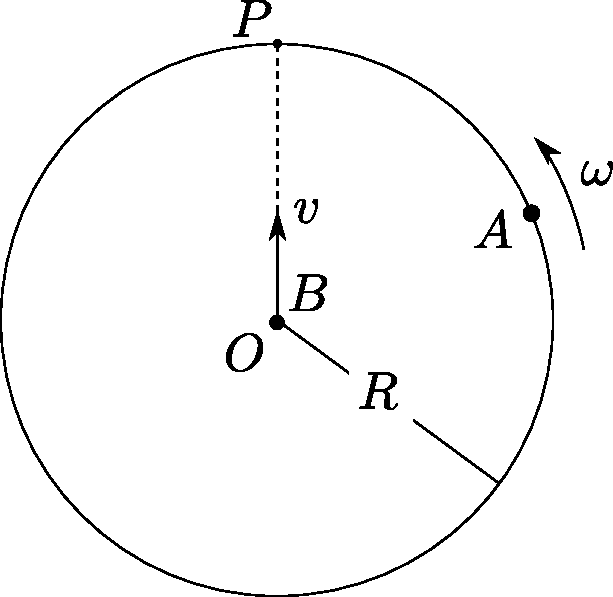
\includegraphics[width = 0.3
\textwidth]{images/motion-problem-9.pdf} 
\end{flushright}
\tagged{student}{\vspace*{4cm}}
\begin{taggedblock}{teacher}
\noindent
解析:质点B运动到圆周所需要的时间$t_B = \frac{R}{v}$,如果它们能够相遇,$A$必须完成若干个完整的周期,也就是
\[
\omega t_B = n\cdot 2\pi
\]
将各个量代入并简化可知
\[
v = \frac{\omega R}{2\pi}\cdot\frac{1}{n},\qquad n=1,2,3\cdots
\]
\end{taggedblock}
\end{example}





\begin{example}
如图所示,质点$A$在半径为$R$的圆周上做角速度为$\omega$的匀速圆周运动。
当它运动到圆周上一给定点$P$时有一质点$B$从圆心$O$从静止出发沿着$OP$方向作匀加速运动,如果两个质点能够相撞,求所有加速度$a$的可能取值。
\begin{flushright}
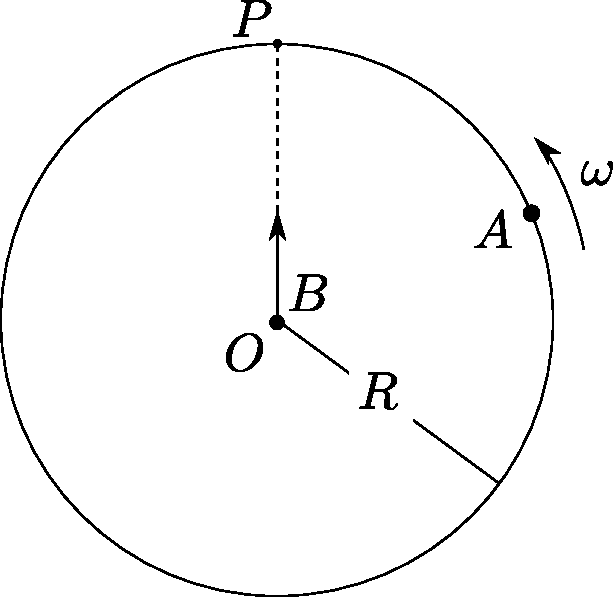
\includegraphics[width = 0.3
\textwidth]{images/motion-problem-10.pdf} 
\end{flushright}
\tagged{student}{\vspace*{4cm}}
\begin{taggedblock}{teacher}
\noindent
解析:这时$B$运动到圆周所需要的时间变成了$t_B = \sqrt{\frac{2R}{a_B}}$,如果它能够和$A$相遇需要满足条件
\[
\omega t_B = n\cdot 2\pi
\]
代数计算表明加速度的可能取值为
\[
a_B = \frac{\omega^2R}{2\pi^2}\cdot\frac{1}{n^2},\qquad n=1,2,3\cdots
\]
\end{taggedblock}
\end{example}

\begin{example}
两个质点在半径为$R$的圆周上分别做匀速圆周运动,角速度分别为$\omega_{1,2}$,并且$\omega_2>\omega_1$,已知$t=0$时两质点在圆周上相遇,求再次相遇的时间。
如图所示,第一次相遇点位于圆心正上方$P$点处,且两质点均沿逆时针方向转动,求再次相遇时的位置与$OP$的夹角$ \theta$。
\begin{flushright}
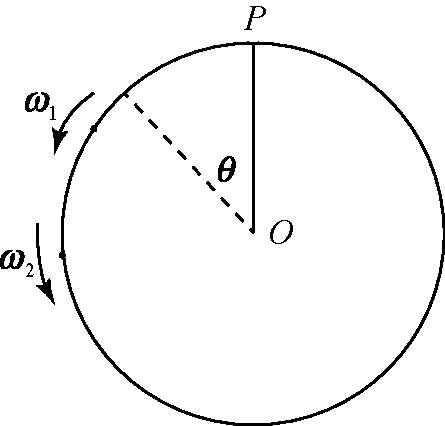
\includegraphics[width=0.4\textwidth]{images/motion-problem-44.pdf}
\end{flushright}
\tagged{student}{\vspace*{1cm}}
\begin{taggedblock}{teacher}
\noindent
解析:这是一个圆周上的追及问题,当两质点的角速度匀为已知时,当它们之间的相对角位移达到$2\pi$时,将再次相遇。
它们之间的相对角速度自然就是它们角速度的差$\omega_2-\omega_1$,所以相遇的时刻满足
\[(\omega_2-\omega_1)t = 2\pi\,\qquad t_= \frac{2\pi}{\omega_2-\omega_1}\]
转过的角度$ \Delta \theta = \omega_1 t$。
\end{taggedblock}
\end{example}

\begin{example}
两个质点$A$和$B$分别在半径为$R_1$、$R_2$的同心圆周上做匀速圆周运动,$A$的线速度为$v_A$,$B$的线速度为$v_B$,当$t=0$时它们连线的沿长线通过圆心且两质点位于圆心的同侧,求此后它们的连线通过圆心的所有时刻。
\begin{flushright}
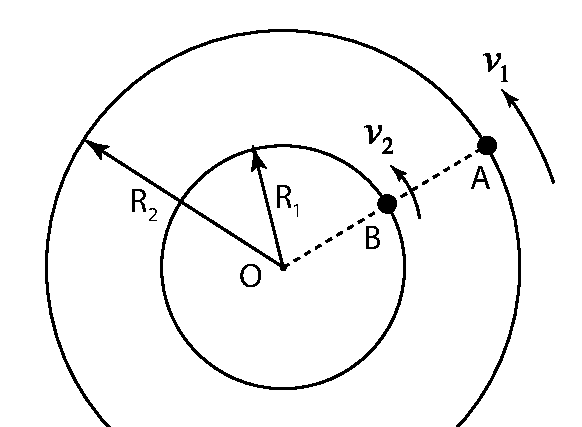
\includegraphics[width=0.4\textwidth]{images/motion-problem-32.pdf}
\end{flushright}
\tagged{student}{\vspace*{2cm}}
\begin{taggedblock}{teacher}
\noindent
解析:两个质点的角速度分别为$ \omega_A = \frac{v_A}{R_1}$、$ \omega_B = \frac{v_B}{R_2}$,利用上一问的结果即可。
\end{taggedblock}
\end{example}



\begin{example}
如图所示,有一个半径为$R$的圆水平放置,有一个质点$A$在其圆周上以角速度$\omega$作匀速圆周运动。
在它圆心$O$的正上方高度为$H$的$S$点以水平速度$v_0$抛出另外一个质点$B$,抛出时$A$正好位于$B$抛出的方向。
如果$B$与$A$能够相撞,则$v_0$和$H$需要满足什么条件。
\begin{flushright}
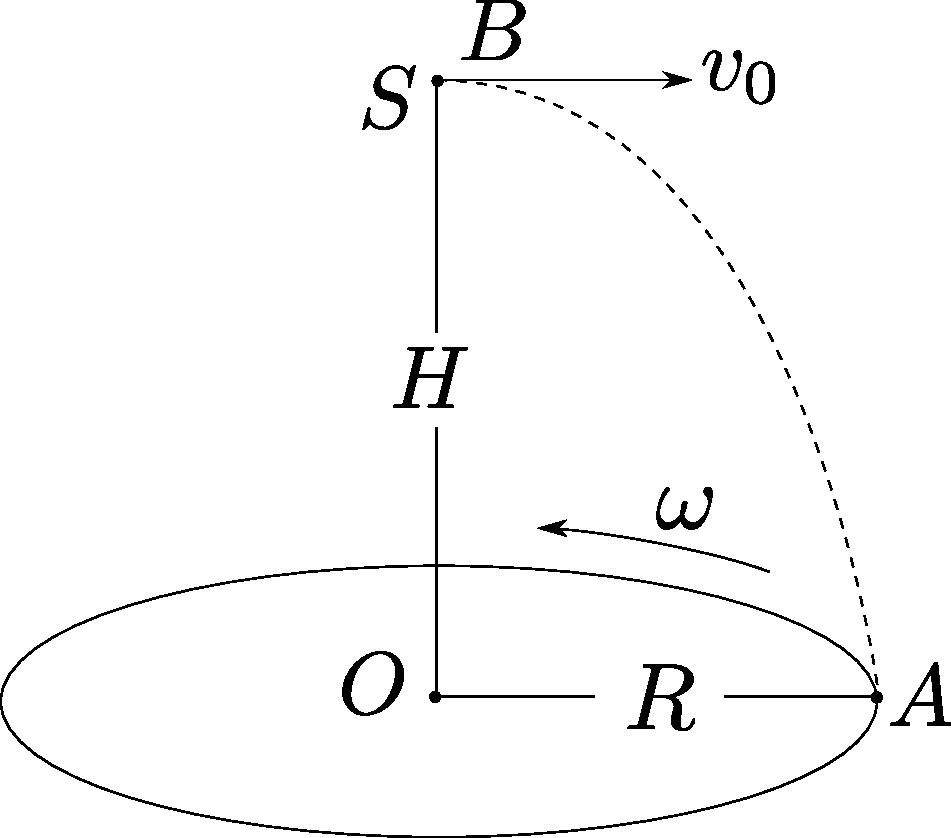
\includegraphics[width = 0.4\textwidth]{images/motion-16.pdf} 
\end{flushright}
\tagged{student}{\vspace*{4cm}}
\begin{taggedblock}{teacher}
\noindent
解析:通过对运动过程的分析可知质点下落过程所需要的时间必须是圆周运动周期的整数倍:
\[
t = \sqrt{\frac{2H}{g}} = nT = n\frac{2\pi}{\omega},\qquad H_n  = \frac{2\pi^2 g}{\omega^2}n^2
\]
水平方向上则要求
\[v_0t = R,\qquad v_n = \frac{\omega R}{2\pi} n\]
两个式子中$n$可取所有自然数。
\end{taggedblock}
\end{example}

\begin{example}
$A$、$B$两个质点在半径分别为$R_1$,$R_2$的同心圆形轨道上同向运动,$R_1<R_2$,角速度分别为$ \omega_1> \omega_2$。
从位于外侧轨道的$B$看过去$A$始终在圆心$O$点左右摆动,求在$B$看来它与$A$和$O$连线之间夹角$ \theta$的最大值以$A$相继出现在最大夹角处的时间间隔。
\begin{flushright}
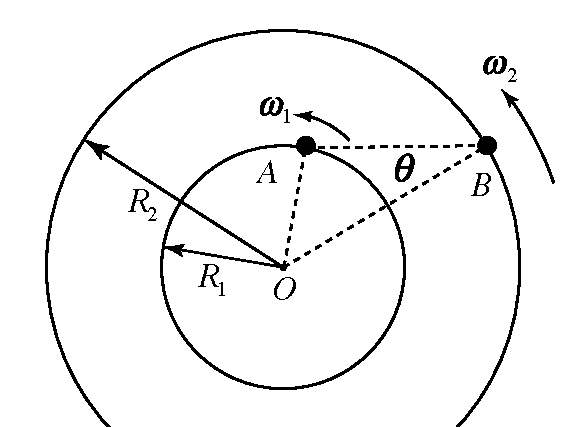
\includegraphics[width=0.4\textwidth]{images/motion-problem-33.pdf}
\end{flushright}

\tagged{student}{\vspace*{4cm}}
\begin{taggedblock}{teacher}
\noindent
解析:通过做图可以发现当外侧质点看到内侧质点张角最大时,两者与圆心连线之间的夹角$\alpha$满足:
\[
\cos\alpha = \frac{R_1}{R_2},\qquad \alpha = \arccos\frac{R_1}{R_2}
\]
这时视线张角
\[
\theta = \frac{\pi}{2}-\alpha.
\]
出现最大角度有两个交替出现的周期,一个是
\[
T_1 = \frac{2\alpha}{\omega_1-\omega_2}
\]
另一个则是
\[
T_2 = \frac{2\pi-2\alpha}{\omega_1-\omega_2}
\]
分别对应于从后向前和从前向后变化的阶段。

\end{taggedblock}
\end{example}











\begin{example}
20世纪早期人们通过实验发现电子有沿着通过自身轴转动的性质。
那时的电子被看成是一个半径$r_e \simeq 3\pow{-15}\unit{m}$,实验上要求电子自转的角速度与半径平方的乘积满足
\[  \omega R^2 \approx 10^{-5}\unit{m^2/s}\]
很短时间之后电子论的创始人洛伦兹马上指出这个模型有致命的缺陷,你能够看出这里面有什么问题吗?
\tagged{student}{\vspace*{4cm}}
\begin{taggedblock}{teacher}
\newline
解析:通过计算能够表明,如果电子的运动的确由上述条件所给出,那么它的边缘运动速度远大于光速。
\end{taggedblock}
\end{example}

虽然匀速圆周运动质点的速度的大小始终不变,但是因为它速度的方向不断发生变化所以加速度并不为零。
如图\ref{fig: motion-匀速圆周运动的加速度}所示一个质点在作半径为$R$角速度为$\omega$的匀速圆周运动,在某一时刻它位于$A$点处,在随后的$\Delta t$时间之后运动到了$B$点,$A、B$两点与圆心的夹角$\Delta\theta = \omega \Delta t$,两点处的速度大小均为$\omega R$,方向沿着两点切线的方向。
为了比较两点速度的不同,将两点的速度矢量平移,使其端点重合于如\ref{fig: motion-匀速圆周运动的加速度}右图所示的$S$点处,连接两个速度矢量的端点$PQ$就是在$\Delta t$时间里速度的变化量。
在极小的时间间隔$\Delta t$内三角形$SPQ$是一个顶角$\Delta\theta=\omega\Delta t$无限地趋近于0,底角无限地趋近于直角的等腰三角形。
因为瞬时加速度的方向就是无限小时间里速度改变量的方向,所以匀速圆周运动的加速方向垂直于瞬时速度,也就是圆周切线的方向;从图中可容易看出其方向指向圆心,所以匀速圆周运动的加速度又被称为{\heiti 向心加速度}。
等腰三角形的腰长$SP=SQ=\omega R$,根据几何关系它的底边的长度为腰长与顶角的乘积:
\[
\Delta v = \omega R \Delta \theta = \omega R\cdot \omega\cdot \Delta t=\omega^2R\Delta t,
\]
可以看到向心加速度的大小与圆周运动的角速度、半径之间的关系
\begin{equation}\label{eqn: motion-a=w^2R}
a_r = \frac{\Delta v}{\Delta t} = \omega^2R,
\end{equation}
根据匀速圆周运动学变量之间的关系,向心加速度还有另外一个常用的表达式:
\begin{equation}\label{eqn: motion-a=v^2/R}
a_r = \frac{v^2}{R}.
\end{equation}
\begin{figure}[hbtp]
\centering
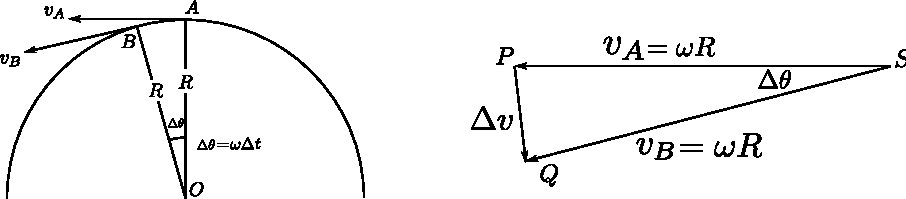
\includegraphics[width=0.9\textwidth]{images/motion-17.pdf}
\caption{匀速圆周运动的加速度}\label{fig: motion-匀速圆周运动的加速度}
\end{figure}



\begin{example}
(1)求一个以线速度$v = 10 \unit{m/s}$在半径$R=10\unit{m}$的圆形轨道上作匀速圆周运动质点的加速度大小。

(2)一个在半径$R = 10\unit{m}$的圆周上匀速圆周运动质点的向心加速度$a_r = 10\unit{m/s^2}$,求其圆周运动的频率。


\tagged{student}{\vspace*{4cm}}
\begin{taggedblock}{teacher}
\noindent
解析:直接根据定义进行计算。第一问
\[a = \frac{v^2}{R} = 10\unit{m/s^2}\]
第二问:
\[
f = \frac{1}{T} = \frac{\omega}{2\pi} = \frac{1}{2\pi}\unit{Hz}.
\]
\end{taggedblock}
\end{example}




\begin{example}
如果多个围绕共同圆心作匀速圆周运动质点的周期$T$的平方与它们各自的轨道半径$R$的三次方成正比:
\[ \frac{T^2}{R^3} = C, \]
其中$C$为一个常数,求它们圆周运动向心加速度与轨道半径的关系。
\tagged{student}{\vspace*{4cm}}
\begin{taggedblock}{teacher}
\newline
解析:假设轨道半径为$R$的质点匀速圆周运动的角速度为$\omega$,其周期
\[ T = \frac{2\pi}{\omega} \]
根据已知的信息可知角速度与半径之间满足
\[  \omega^2 = \frac{4\pi^2}{CR^3}, \]
这样不同半径上质点的向心加速度为
\[ a_r = \omega^2R = \frac{4\pi^2}{CR^2}, \]
可见向心加速度与它们到圆心距离的平方成反比。
当把这两个例子应用到动力学中的时候恰恰代表了两种最经典的有心力情况下的运动。
\end{taggedblock}
\end{example}

\begin{example}
如果多个围绕共同圆心作匀速圆周运动质点的周期$T$与它们各自的轨道半径$R$无关,求向心加速度与轨道半径之间的关系。
\tagged{student}{\vspace*{4cm}}
\begin{taggedblock}{teacher}
\newline
解析:和前一问几乎一模一样的做法,只不过周期和半径的关系发生了变化,简单的代数计算表明这时的向心加速度需要和轨道半径$R$成正比:
\[a_r = \frac{4\pi^2}{T^2}R\]
\end{taggedblock}
\end{example}




\begin{example}
以圆形轨道行驶的赛车速度不宜过快,否则就会打滑,已知在给定的赛道上赛车沿不同圆周作匀速运动的向心加速度的最大值均为$a$,它同时也是赛车在加速度和减速过程中的最大加速度。
考虑如图所示赛道,弯道为圆孤,内、外半径分别为$R_1$、$R_2$。
在直道上赛车以最大速度$v_0>\sqrt{aR_1}$,比较沿着赛道内侧和外侧两种方式通过弯道的时间。
\begin{flushright}
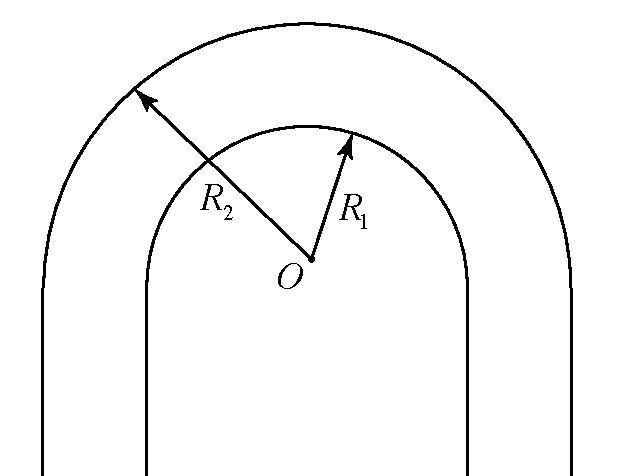
\includegraphics[width=0.4\textwidth]{images/motion-problem-34.pdf}
\end{flushright}
\tagged{student}{\vspace*{4cm}}

\begin{taggedblock}{teacher}
\noindent
解析:略
\end{taggedblock}
\end{example}

在大多数情况下,圆周运动的角速度并不是一直能够不变的,在各种因素的影响下和质点运动的速度一样,角速度也会发生变化。
把圆周运动质点的角位置在一段时间$\Delta t$内的变化量$\Delta\theta$与相应的时间间隔的比值称为$\Delta t$时间里的平均角速度,和速度类似的在极小的$\Delta t$极限下平均角速度的极限就是对应时刻的瞬时角速度:
\begin{equation}
\omega(t) = \lim_{\Delta t\rightarrow 0 }\frac{\Delta \theta}{\Delta t}
\end{equation}
当圆周运动质点在某一时刻的瞬时角速度为已知时,可以证明它的线速度和向心加速度满足和匀速圆周运动相同的规律:
\begin{equation}
v(t) = R\omega(t),\qquad a_r=\omega(t)^2R = \frac{v(t)^2}{R}
\end{equation}


和直线运动相类比,当角速度做为时间的函数为已知时,它对时间的变化率自然就被称为{\heiti 角加速度},习惯上用$\beta$来表示。
如果角速度随时间的关系用函数$\omega(t)$来表示的话,角加速度也以写为
\begin{equation}
\beta(t) = \lim_{\Delta t\rightarrow 0}\frac{\Delta \omega}{\Delta t}.
\end{equation}
当圆周运动的角加速不为零时,运动质点的加速度除了指向圆心的分量以外还会由于线速度的变化有沿着圆周切线方向的分量,称为{\heiti 线加速度}或{\heiti 切向加速度}。
简单的数学分析可知线加速度的大小
\begin{equation}\label{eqn: motion-线加速度}
a_t = R\beta
\end{equation}
这时运动质点的加速度为切向加速度和向心加速度的矢量和。
线加速度保持为常数的圆周运动称为{\heiti 匀加速圆周运动},如果$t=0$的初始时刻以角加速度$\beta$作匀加速圆周运动质点的初始角位置为$\theta_0$、初始角速度$\omega_0$的质点的角速度和角位置随时间的变化关系可以写为
\begin{eqnarray}
\omega(t)&=&\omega_0+\beta t\\
\theta(t)&=&\theta_0+\omega_0t+\frac{1}{2}\beta t^2
\end{eqnarray}
作角加速运动的质点速度的大小和方向都在不断变化,由于角加速度不为零,所以质点运动过程中沿着圆周切向的加速度分量\ref{eqn: motion-线加速度}以外,速度方向的改变同时也会导至非零的径向加速度分量,简单地分析可知向心加速度同样是由\ref{eqn: motion-a=v^2/R}给出,只不过这时式中的$v^2$在不同的时间需要取不同的数值。



\begin{example}
一质点在半径为$R=1\unit{1}$圆周上作圆周运动,$t=0$时初始角速度为$\omega_0=0$,角加速度$\beta = 1\unit{rad/s^2}$,求其边缘速度达声速$340\unit{m/s}$所需要的时间。
\tagged{student}{\vspace*{4cm}}
\begin{taggedblock}{teacher}
\newline
解析:任意时刻的线速度由
\[v = \omega(t)R = \beta R t\]
这样超过声速的时刻自然就是
\[
t' = \frac{v_S}{\beta R}\simeq 340\unit{s}
\]
\end{taggedblock}
\end{example}


%%%%%%%%%%%%%%%%%%%%%%%%%%%%%%%%%%
\begin{example}
一质点沿半径为$R$的圆轨道运动,初速度为$v_0$,其加速度方向与速度方向之间的夹角$ \theta$恒定,试求速度大小与时间的关系。
\begin{flushright}
\includegraphics[width=0.3\textwidth]{images/motion-problem-41.pdf}
\end{flushright}
\tagged{student}{\vspace*{1cm}}
\begin{taggedblock}{teacher}
\noindent
解析:【选讲】设加速度的大小为$a$,未知。在径向和横向上运动分别满足:
\[
a\cos\theta = \frac{v^2}{R},\qquad \frac{\Delta v}{\Delta t} = a\sin\theta.
\]
联立以上两式消去$a$可得速度随时间的变化关系
\[
\frac{\Delta v}{\Delta t} = \frac{v^2}{R}\tan\theta,
\]
该方程的解为
\[
v(t) = \frac{1}{\frac{1}{v_0}-\frac{\tan\theta}{R}t}
\]
\end{taggedblock}
\end{example}











\section{平面内的曲线运动}
详细地研究了抛体和圆周运动以后,我们已经积累了大量的描述物体运动的手段和技术。
在这些技术的基础上就可以着手分析更一般的运动,为简单起见假设运动物体始终保持在空间当中某个特定的平面内,称之为二维运动;后面可以看出对二维运动的研究对更复杂的三维运动的描写提供了几乎全部的术语和技术,向三维空间的推广几乎不用费任何力气。
对二维曲线运动的分析主要采取两种方法,一种是在平面直角坐标系或极坐标系中用物体在坐标系的分量随时间的变化来描写物体的运动;另一种是时刻追随运动的物体,将它所有的运动学变量在它的速度方向和垂直于速度的方向来分解从而得到运动的性质。
两种方法各有特点和优势,根据实际的问题选择合适的处理方法,下面我们就来逐一学习两种不同的描写手段。

\subsection{固定坐标系}
\begin{figure}[hbtp]
\centering
\includegraphics[width=0.5\textwidth]{images/motion-18.pdf}
\caption{用直角坐标系描写质点的曲线运动,用质点的坐标随时间的关系来决定任一时间运动质点的位置。当根据运动方程得到$t_1$时刻的两个坐标值分别为$x(t_1)$和$y(t_1)$,立刻就可以判断质点此时位于图中的$A$点处}\label{fig: motion-曲线运动的直角坐标系描写}
\end{figure}

在质点运动的平面内建立一个直角坐标系$Oxy$,其中$O$为坐标系的原点,$x、y$分别是相互垂直的两根坐标轴。
对于轴的取向并没有特别的规定,可以根据所研究对象运动的特点灵活选择。
例如处理抛体运动时选择两根轴分别平行和垂直于地面就很方便,另外在处理地面上物体的运动时将轴指向东西和南北方向可以更方便地与地理知识产生联系。
当坐标系被给定了以后,平面内任何一点的坐标就是被唯一给定的,反过来当给定了一个物体的两个坐标值以后它真实的位置也将被唯一确定。
物体的运动可以用它的两个坐标值分别与时间的关系来描写,如图\ref{fig: motion-曲线运动的直角坐标系描写}所示对于坐标系$Oxy$来说平面内质点的运动可以用它的$x$和$y$坐标与时间的函数给出:
\begin{equation}\label{eqn: motion-分量的运动方程}
x = x(t),\qquad y = y(t)
\end{equation}
$x(t)$和$y(t)$称为曲线运动分量的运动方程,无论多么复杂的曲线运动其分量看上去都是在作一维的运动,可以用一维运动的相应技术来分析分运动,最后就可以得到完整的运动。
在抛体的运动分析过程中我们已经看到,当把抛体的运动分解为水平和竖直方向的分运动以后就可以简单地分析了。
当分量的运动方程\ref{eqn: motion-分量的运动方程}为已知时,就能够得到曲线运动的其它信息。

运动物体的轨迹可以由各个时刻的位置在平面上划出的曲线所决定。
从数学上看和抛体运动类似,任意曲线运动的轨迹可以通过联立两个方向分运动的方程通过消去时间变量而得。
在有些特殊情况下很容易得到轨迹的方程,但不见得所有情况下都能够得到轨迹方程解析的表达式。



\begin{example}
已知分量的运动方程为
\[x(t) = A\cos\omega t,\qquad y(t)=A\sin\omega t\]
求运动质点的轨迹方程并在下面的坐标系中画出轨迹的示意图。
\begin{flushright}
\includegraphics[width=0.4\textwidth]{images/motion-problem-35.pdf}
\end{flushright}
\tagged{student}{\vspace*{0cm}}
\begin{taggedblock}{teacher}
\noindent
解析:很明显是一个圆,两式取平方和就可以消去时间,可以得到轨迹满足
\[x^2+y^2 = A^2\]
很明显是平面内圆的方程。
\end{taggedblock}
\end{example}

\begin{example}
已知分量的运动方程为
\[x(t) = a\cos\omega t,\qquad y(t)=b\sin\omega t\]
求运动质点的轨迹方程,并画出轨迹的示意图。
\begin{flushright}
\includegraphics[width=0.4\textwidth]{images/motion-problem-35.pdf}
\end{flushright}
\tagged{student}{\vspace*{0cm}}
\begin{taggedblock}{teacher}
\noindent
解析:轨迹是一个椭圆,将两式右边的$a$、$b$除到左边来再求平方和就可以消去时间,得到
\[\frac{x^2}{a^2}+\frac{y^2}{b^2}=1\]
是平面内椭圆的方程。
\end{taggedblock}
\end{example}



\begin{example}
一个半径为$R$的圆在平面上以做无滑动的匀速滚动,圆心速度速度为$v$,试求圆上固定一点$P$在如图所示的坐标系中$x、y$坐标随时间的函数。
\begin{flushright}
\includegraphics[width = 0.5\textwidth]{images/motion-19.pdf}  
\end{flushright}
\tagged{student}{\vspace*{4cm}}
\begin{taggedblock}{teacher}
\noindent
解析:运动学的分析表明经过$t$的时间里转过部分相对圆心的夹角为$\frac{v}{R}t=\omega t$,由几何关系可知点$P$的运动方程为
\[
x_p(t) = R[\omega t - \sin\omega t],\qquad y_p(t) = R[1-\cos\omega t]
\]
\end{taggedblock}
\end{example}




\begin{example}
已知一个在空间中运动的质点在直角坐标系$Oxyz$中的运动方程为
\[x(t) = R\cos\omega t,\qquad y(t) = R\sin\omega t,\qquad z(t) = vt \]
以上各量均为正数,试画出质点轨迹的示意图。
\begin{flushright}
\includegraphics[width=0.4\textwidth]{images/motion-problem-36.pdf}
\end{flushright}
\tagged{student}{\vspace*{0cm}}
\begin{taggedblock}{teacher}
\noindent
解析:$x-y$平面上作匀速圆周运动,在$z$方向上匀速运动,总得来看就是一个旋转上升的螺旋线。
\end{taggedblock}
\end{example}

曲线运动的速度可以由分运动速度的矢量和给出。
对于由\ref{eqn: motion-分量的运动方程}给出的运动,它在坐标轴的分速度自然为已知,这样它的速度可以由两个方向的速度合成而得。
反过来的过程也是成立的,当已知曲线运动在某一时刻的速度以后它分的分速度可由速度沿坐标轴的分量而得到。
同样的道理运动质点的加速度也等于分量的加速度的矢量和,加速度的分量等于总的加速度在对应轴的分量。

\begin{example}
现有一个质点$P$在半径为$R$的圆上作角速度为$\omega$的匀速圆周运动。
建立一个原点位于圆心$O$的平面直角坐标系,在$t=0$的时刻质点刚好处于$x$轴上,且围绕原点做逆时针转动。
求此后任意时间它在坐标轴上的投影$x(t) = R\cos\omega t$,$y(t) = R\sin\omega t$的速度和加速度。
\begin{flushright}
\includegraphics[width = 0.4\textwidth]{images/motion-35.pdf} 
\end{flushright}
\tagged{student}{\vspace*{4cm}}
\begin{taggedblock}{teacher}
\noindent
解析:当速度的分量为已知时,可以得到真实速度的大小和方向。
反过来,当知道了质点运动的速度以后,它向着各个方向投影点速度的大小和方向也能够反过来得到。
对于这个圆周运动的例子来说,沿圆周运动的速度和加速度均为已知,只需要将它们投影到各个坐标轴上就可以得到运动质点在坐标轴上投影的速度和加速度。
质点运动方程中的$\omega t$决定了投影的角度。
它在运动过程中的速度大小均为$v=\omega R$,方向沿着圆的切线;加速度大小均为$a = \omega^2R$,方向指点圆心。
通过上面的分析很容易得知,它在$x$、$y$轴的投影运动的速度和加速度分别为
\begin{eqnarray*}
&v_x = -\omega R \sin \omega t,\qquad & a_x = -\omega^2 R\cos\omega t\\
&v_y = \omega R \cos \omega t,\qquad & a_y = -\omega^2R\sin\omega t
\end{eqnarray*}

\end{taggedblock}
\end{example}





\begin{example}
试证明一个半径为$R$的圆在平面上以做无滑动的匀速滚动,圆心速度速度为$v$,当圆上固定一点$P$刚好与地面接触时的瞬时速度为零。
\begin{flushright}
\includegraphics[width = 0.4\textwidth]{images/motion-36.pdf} 
\end{flushright}
\tagged{student}{\vspace*{4cm}}
\begin{taggedblock}{teacher}
\noindent
解析:各种方法证明均可,无滑动的话自然这一点的速度必须为零。
\end{taggedblock}
\end{example}


\begin{example}
在如图所示的平面极坐标系中,一个质点的运动由方程
\[ r = vt,\qquad  \theta  = \omega t\]
给出,所有参数均为正数,试定性地画出其运动轨迹。
\begin{center}
\includegraphics[width=0.3\textwidth]{images/motion-problem-37.pdf}
\end{center}
\tagged{student}{\vspace*{0cm}}
\begin{taggedblock}{teacher}
\noindent
解析:在极坐标系中,运动质点与原点的距离随时间均匀增大,同时角度也均匀增大,可以想像到的时运动轨迹为某种形式的螺线形。
\end{taggedblock}
\end{example}


\begin{example}
在平面极坐标系中一个质点的运动由方程
\[
r = r_0 e^{\lambda t},\qquad \theta=\omega t
\]
试证明它在任何一点处的速度与它到极坐标系中心连线的夹角均为给定值,并给出该值。
已知对于任意的$x$,当其变化量$\Delta x\ll x$时,有如下的近似关系式:
\[e^{x+\Delta x}\simeq e^x(1+\Delta x)\]
\tagged{student}{\vspace*{4cm}}
\begin{taggedblock}{teacher}
\newline
解析:运动质点与中心的距离随时间指数增加,而角度则是均匀增大,轨迹也是某种形式的螺线形。
对于任意的时刻$t$以及其随后的微小时间间隔$\Delta t$,其径向距离变成了:
\[ r(t+\Delta t) =r_0 e^{\lambda (t+\Delta t)}\simeq r_0e^{\lambda t}(1+\lambda \Delta t)=r(t)(1+\lambda \Delta t)\]
这样其径向距离的变化量则是:
\[
\Delta r = r(t)\lambda\Delta t
\]
在同样的时间里,它的横向位置的变化量则是
\[ r(t)\Delta \theta  = r(t)\omega\Delta t \]
与径向距离的变化量相比可以看出
\[
\frac{\Delta r}{r \omega \Delta t} = \frac{\lambda}{\omega}=const
\]
\end{taggedblock}
\end{example}
\subsection{自然坐标系}
除了用运动平面内的直角坐标系,还可以在平行和垂直于曲线运动物体速度的方向将各个运动学变量分解。
这里将与速度相同的方向称为运动的{\heiti 切线方向},简称{\heiti 切向},故名思意切向就是运动轨迹切线的方向。
与切线垂直,指向运动轨迹弯曲的方向称为轨迹的{\heiti 法线方向},简称{\heiti 法向}。
根据运动学性质,曲线运动质点的速度只有切向分量,法向分量为零。
但是加速度则不同,作曲线运动物体加速度必然与瞬时速度方向不一致,所以加速度即有切向分量,也有法向分量。
由运动轨迹的切向和法向构成的坐标系称为{\heiti 自然坐标系},运动学变量在自然坐标系中的分量具有最明确的物理意义,但是由于曲线运动质点的切向和法向在其轨迹上不同点处的方向并不一样,所以在自然坐标系是一个方向不断发生变化的坐标系,在它里面处理运动学问题有一定的数学复杂性。


\begin{figure}[hbtp]
\centering
\includegraphics[width = 0.5\textwidth]{images/motion-20.pdf}
\caption{曲线运动速度的变化量,当$\Delta t\rightarrow 0$时可以理解加速度在自然坐标系中分量的物理含义}
\label{fig: motion-曲线运动速度的变化}
\end{figure}

假设曲线运动质点在某一给定时刻$t$时的位置矢量由$\vec{r}(t)$给出,此时的瞬时速度和瞬时加速度由矢量$\vec{v}$,$\vec{a}$给出。
在此之后的$\Delta t$时间后,它的位置和速度会发生一定的变化,如果时间间隔选取足够小的话,可以认为在$\Delta t$时间里做匀加速度直线运动,这样$t+\Delta t$时刻的速度和位置分别由
\begin{eqnarray}
\vec{v}(t+\Delta t)& = &\vec{v}+\vec{a}\Delta t\label{eqn: motion-曲线运动速度变化量}\\
\vec{r}(t+\Delta t)& =& \vec{r}(t)+\vec{v}\Delta t+\frac{1}{2}\vec{a}\Delta t^2\label{eqn: motion-曲线运动中位置的变化量}
\end{eqnarray}
给出。
我们来着重考察曲线运动物体速度的变化量,式\ref{eqn: motion-曲线运动速度变化量}的图形表示如图\ref{fig: motion-曲线运动速度的变化},从中可以看出在最一般的情况下由于非零的加速度会导致速度的大小和方向同时发生变化。
在无限小的$\Delta t$间隔里,图中的三角形$ABC$实际上是一个顶角$\Delta \theta$极其之小的三角形,在后面的推理过程中要密切注意这一点。
各条边的长度已经在图中标出,$\alpha$角代表瞬时加速度$\vec{a}$与瞬时速度$\vec{v}$的夹角。
速度大小的变化量由图中边长$AC$与$AB$的差别来表示,而速度方向的变化可以由$\Delta \theta$来表达。


在三角形$ABC$中使用余弦定理可得
\[
v(t+\Delta t) = \sqrt{v(t)^2+a^2\Delta t^2+2va\Delta t\cos\alpha}
\]
与通常的余弦定理不同的是$\alpha$是三角形的外角,所以上式中最后一项的符号为正。
在$\Delta t\rightarrow 0$的极限下可以忽略所有$\Delta t$一次方项以外的其它高次项,并将上式做近似展开:
\begin{eqnarray*}
v(t+\Delta t)&=&v(t)\left(1+2\frac{a}{v}\Delta t\cos\alpha\right)^{1/2}\\
& \simeq & v(t)\left( 1+ \frac{a}{v}\cos\alpha\Delta t \right) = v(t)+a\cos\alpha \Delta t
\end{eqnarray*}
从中可以看到速度大小的变化量
\[
\Delta v = v(t+\Delta t)-v(t) = a\cos\alpha\cdot \Delta t
\]
结合图\ref{fig: motion-曲线运动速度的变化}能够看到,速度大小的变化量等于加速度在沿速度方向的分量,也就是加速度的切向分量$a\cos\alpha$与时间间隔$\Delta t$的乘积。
也就是说加速度的切向分量能够决定曲线运动速率的变化,当加速度的切向分量与速度方向一致时运动速率将会增加,反之当加速度的切向分量与速度相反时曲线运动的速率会减小,最特殊的情况下当加速度与速度方向垂直时,运动速率不会发生任何变化,这一点在匀速圆周运动的例子中已经看到。

速度方向的变化用图\ref{fig: motion-曲线运动速度的变化}中的角度$\Delta\theta$来衡量,在小角度极限下角度的弧度值、正弦值和正切值在数字上近似相等。
在三角形$ABC$中利用正弦定理有
\[
\frac{v(t+\Delta t)}{\sin\alpha}=\frac{a\Delta t}{\sin\theta}
\]
简单的数学运算并略去更小的量以后上式可以整理成为
\begin{equation}
\Delta\theta = \frac{a\sin\alpha }{v}\Delta t
\end{equation}
从中可以看出加速度的法向分量的大小和运动速率共同决定了速度方向变化的快慢。
将上式变形可以得到
\[
a\sin\alpha = v\frac{\Delta\theta}{\Delta t},
\]
最后一个因子看上去和一个圆周运动角速度的表达式非常相似,如果假想圆周运动的线速度就是曲线运动质点在此时的速率,半径为$\rho$,那么它可以表示为
\begin{equation}
a\sin\alpha = v\frac{v}{\rho} = \frac{v^2}{\rho}
\end{equation}
它很像匀速圆周运动的向心加速度的表达式。
可以形象将曲线运动质点在其轨迹上任何一点处的运动与一个圆周运动等同起来,圆周运动的线速度就是曲线运动质点的瞬时速率,半径由上式中$\rho$给出,它由曲线运动质点速度方向的变化量所决定。
数学上将这个等效的圆周运动的圆形称作曲线运动轨迹的{\heiti 密切圆},它完全由曲线的形状所决定,图\ref{fig:Osculating_circle}给出密切圆的一个例子。
关于密切圆,有一个形象的理解。
回忆一下一些基本的几何事实:两个点唯一决定一条直线,直线上无限接近的两点之间连线的极限就是曲线的切线;与之相似的,不在同一直线上的三个点唯一地决定了一个圆,在曲线上一点的两侧取两个点,让这两个点无限地逼近给定点的过程中它们与给定点所决定的圆的极限就是曲线的密切圆。

\begin{figure}[ht]
\centering
\includegraphics[width=0.5\textwidth]{images/Osculating_circle}
\caption{曲线上任意一点处的密切圆}
\label{fig:Osculating_circle}
\end{figure}


\begin{example}
抛体运动的上升过程中加速度和速度夹角为$\underline{\qquad }$(锐,钝)角,运动速率不段$\underline{\qquad }$(增加,减小);下降过程中加速度与速度夹角为$\underline{\qquad }$(锐,钝)角,速率不段$\underline{\qquad }$(增加,减小)。
确定抛物线$y = ax^2$在$x=0$处的曲率半径。
\tagged{student}{\vspace*{4cm}}
\begin{taggedblock}{teacher}
\newline
解析:从原点出发平抛的运动方程$y=-\frac{gx^2}{2v_0^2}$,此时加速度大小为$g$,方向向下。
设此时的曲率半径为$\rho$,根据密切圆的性质可得
\[
\frac{v^2}{\rho} = g,\qquad \rho = \frac{v^2}{g}
\]
因为密切圆只与曲线形状有关,将上式与平抛轨迹方程做比较可知当抛物线用$y = ax^2$来表示时在最底点的曲率半径
\[
\rho = \frac{1}{2a}
\]

\end{taggedblock}
\end{example}

\begin{example}
评估下面这条曲线上四个点的弯曲情况,并尽可能地画出这些点的密切圆。
\begin{center}
\includegraphics[width=0.7\textwidth]{images/motion-problem-curved-lines-radius.pdf} 
\end{center}


\end{example}

\begin{example}
求长轴、短轴分别为$a、b$的椭圆在其长轴和短轴处的曲率半径。
\begin{flushright}
\includegraphics[width=0.3\textwidth]{images/motion-problem-45.pdf}
\end{flushright}
\tagged{student}{\vspace*{4cm}}
\begin{taggedblock}{teacher}
\noindent
解析:前面已经分析了椭圆轨道运动质点两个分量随时间的变化关系,当运动到长轴时加速度只有$x$分量,大小为$-\omega^2 a$,而速度只有$y$分量,大小则是$\omega b$,这样根据曲线运动的一般性质它的加速度垂直于速度,只有横向分量:
\[
\omega^2a = \frac{\omega^2b^2}{\rho_a},\qquad \rho_a = \frac{b^2}{a}
\]
同样的道理在短轴处
\[
\rho_b = \frac{a^2}{b}
\]
\end{taggedblock}
\end{example}

\begin{example}
有一个沿直线运动的质点,在$t=0$时刻速度为$v_0$并作减速运动,此后任意时刻的加速度与速度方向相反,且正比于当时的速度值$a=-kv$,求它完全停止所需要的时间和走过的总路程。
%\begin{flushright}
%\includegraphics[width = 0.2\textwidth]{images/.pdf} 
%\end{flushright}
\tagged{student}{\vspace*{4cm}}
\begin{taggedblock}{teacher}
\newline
解析:【选讲】可利用微元法讲解。
满足已知条件时速度随时间$t$和前进距离$x$变化关系为
\[
v(t) = v_0e^{-kt},\qquad v = v_0-kx
\]
\end{taggedblock}
\end{example}


\begin{example}
有一个沿直线运动的质点,在$t=0$时刻速度为$v_0$并作减速运动,此后任意时刻的加速度与速度方向相反,且正比于当时的速度值的平方$a=-\beta v^2$,求它速度随时间的变化关系。
\tagged{student}{\vspace*{4cm}}
\begin{taggedblock}{teacher}
\newline
解析:【选讲】速度随时间的变化关系为
\[
\frac{1}{v(t)} = \frac{1}{v_0}+\beta t,\qquad v(t) = \frac{v_0}{1+ v_0\beta t}
\]
\end{taggedblock}
\end{example}

\section{天体运动:太阳系的运行}
\begin{figure}[h]
\centering
\includegraphics[width=0.5\textwidth]{images/motion-Kepler_Mars_retrograde.pdf}
\caption{地球上看到的火星运动轨迹}
\label{fig:motion-Kepler_Mars_retrograde}
\end{figure}

在人类历史的很长一段时间里,人们都认为地球是宇宙的中心,太阳、月球、行星和所有的恒星都围绕地球做匀速圆周转动,这就是长期以来一直坚持的{\heiti 日心说}。
日心说在解释太阳、月球、恒星围绕地球的转动并没有什么问题,但是在试图解释行星的运行时却遇到了几乎无法克服的困难。
天文学家哥白尼指出如果假设地球和所有其它行星一起共同围绕太阳转动,那么在解释太阳系的运行时就简单了许多,经过和传统观念的长期斗争最终{\heiti 日心说}取得了胜利。
在日心说建立早期,由于观测数据不完备,也由于人们对自然界物体运动存在有一些非科学的看法,认为地球和行星围绕太阳做匀速圆周运动,但随着人们观测手段的进步并经过长期精确的天文观测以后发现行星围绕太阳的运行轨迹并不是严格的圆形,在轨道不同位置处速度也不一致。

最终天文学家开普勒在大量观测数据的基础上总结出了行星运动的三个经验定律,称为{\heiti 开普勒三定律},它们分别是
\begin{enumerate}
\item 行星的轨道是一个椭圆,太阳位于椭圆的一个焦点上。
\item 行星与太阳的连线在相同时间里扫过相同的面积。
\item 行星运行周期的平方与椭圆轨道半长轴的立方的比值对于所有行星均相同。
\end{enumerate}
按照顺序它们分别称为开普勒第一、第二和第三定律。
第一和第二定律是针对单个行星来说的,而第三定律是不同行星公转参数之间的一个关系。
开普勒定律为近代科学的发展打开了一道大门,最终牛顿在开普勒三定律的基础上建立了近代力学的体系。
我们只有先在运动学的范围内将天体的运动分析清楚以后才能够进一步地分析天体运动的其它特征。
从开普勒定律当中可以看出,行星的运动都是椭圆轨道上的曲线运动,利用前面掌握的分析曲线运动的技术就能够在一定程度上更精确地掌握行星的运动学特征,尤其是在行星在运行过程中速度和加速度的变化与它的位置,特别是和太阳的距离之间究竟满足什么样的关系。


\subsection{开普勒第一定律:椭圆}
\begin{figure}[hbtp]
\centering
\includegraphics[width=0.45\textwidth]{images/motion-ellipse-detail.pdf}  
\includegraphics[width=0.3\textwidth]{images/motion-21.pdf} 

\caption{椭圆中的各个相关几何量及其定义}\label{fig: motion-椭圆的定义}
\end{figure}


开普勒第一定律给出了轨道的形状以及和太阳的相对位置关系。
椭圆是一个之前不太熟悉的几何图形,简单地说椭圆就是圆在平面上的投影,或者说是一个被“挤扁”了的圆。
从数学上看椭圆还可以被看成是到两个给定点距离之和等于常数的所有点构成的集合。
如图\ref{fig: motion-椭圆的定义}中所给出的,这两个给定点分别为$F_1$和$F_2$,它们称为椭圆的两个{\heiti 焦点},开普勒第一定律指出当图中的椭圆代表某颗行星的轨道时,太阳必然位于$F_1$或$F_2$处。
通过对称性和椭圆的定义很容易证明,椭圆上一点到两个焦点距离之和正是椭圆当中最长的那条线$A_1A_1$的长度。
$A_1A_2$称为椭圆的{\heiti 长轴},它的中点$C$就是椭圆的中心,$CA_1=CA_2=a$称为椭圆的半长轴,它出现在开普勒第三定律当中。
与长轴相应地还有一条短轴,在图中用$CB_1=CB_2=b$表示,长轴和短轴的长度就唯一确定了椭圆的形状,并且从中可以看出当长轴与短轴长度相同时椭圆就退变成了一个圆。
除了长轴和短轴以外,中点到焦点的距离$CF_1=CF_2=c$也是椭圆的一个重要的特征量,它称为椭圆的{\heiti 半焦距},自然两焦点之间的距离就是椭圆的{\heiti 焦距}。
半焦距$c$与半长轴$a$的比值称为椭圆的偏心率
\begin{equation}
e = \frac{c}{a},
\end{equation}
偏心率是描写椭圆更圆一些或更扁一些的物理量,$e=0$的极限情况下椭圆就退化为一个圆,从这个角度来说圆可以看做是偏心率为零的椭圆,对于椭圆来说$0<e<1$,偏心率越大椭圆就越扁,反之偏心率越小椭圆就越圆。
建立图\ref{fig: motion-椭圆的定义}所示的平面直角坐标系,原点和椭圆的中点重合,$x$轴和$y$轴分别与长轴和短轴重合,这样椭圆上所有的点满足方程
\begin{equation}
\frac{x^2}{a^2}+\frac{y^2}{b^2}=1.
\end{equation}




\begin{example}
证明在椭圆当中$a^2=b^2+c^2$,在此基础上将半短轴长度$b$用$a$和$e$表示出来。
\begin{flushright}
\includegraphics[width = 0.3\textwidth]{images/motion-37.pdf} 
\end{flushright}
\tagged{student}{\vspace*{2cm}}
\begin{taggedblock}{teacher}
\noindent
解析:由短轴的顶点、中心点和一个焦点做一个直角三角形,三条边的长度分别为$a$、$b$和$c$,在三角形当中使用勾股定理可以证明该结论。
进一步可以根据偏心率的定义可知
\[
b=\sqrt{a^2-c^2}=\sqrt{a^2-a^2e^2} = a\sqrt{1-e^2}
\]
\end{taggedblock}
\end{example}

\begin{example}
用椭圆的半长轴$a$和偏心率$e$写出椭圆面积的表达式。
\tagged{student}{\vspace*{4cm}}
\begin{taggedblock}{teacher}
\newline
解析:椭圆是圆的投影,所以它的面积也等于圆面积在平面上的投影。
简单的分析可知椭圆面积$S=\pi ab$,根据前面一问的答案可知
\[S=\pi a b = \pi a^2\sqrt{1-e^2}\]
\end{taggedblock}
\end{example}

\begin{example}
行星轨道上距离太阳最近的点称为近日点,与太阳相距最远的点称为远日点。
求当一颗行星在半长轴为$a$,偏心率为$e$的椭圆轨道上运动时近日点和远日点的距离。
\begin{flushright}
\includegraphics[width = 0.4\textwidth]{images/motion-38.pdf} 
\end{flushright}
\tagged{student}{\vspace*{4cm}}
\begin{taggedblock}{teacher}
\noindent
解析:根据椭圆中各个量的定义,半长轴为$a$,偏心率为$e$时轨道的半焦距
\[
c = ae
\]
从几何上可以看出近日点和远日点与太阳的距离分别为
\[ r_1 = a(1+e),\qquad r_2 = a(1-e) \]
\end{taggedblock}
\end{example}






\subsection{开普勒第二定律}
\begin{figure}[hbtp]
\centering
\includegraphics[width=0.7\textwidth]{images/motion-22.pdf}
\caption{开普勒第二定律:相同时间里矢径扫过相同的面积}\label{fig: motion-开普勒第二定律解释}
\end{figure}


开普勒第一定律给出了行星轨道的形状和太阳的位置,第二定律告诉了我们轨道上的行星位置是如何随时间变化的。
与直线运动不同的是做曲线运动的行星与太阳连线(矢径)扫过的面积与时间成正比,一段时间矢径扫过的图形为一个类似于图\ref{fig: motion-开普勒第二定律解释}左面所示的扇形的几何图形$SP_1P_2$,其面积并不容易计算。
但在一段极其之小的时间里行星的运动可以近似地看成是匀速直线运动,在这样的小的时间里行星矢径扫过的面积可以近似地看成一个顶角很小的三角形,它的面积可以通过行星的速度以及它对太阳的位置所决定。

如图\ref{fig: motion-开普勒第二定律解释}右图所示,在某一时刻$t$行星位于轨道上的$P$点处,它的速度与椭圆相切,大小为$v$,已在图中标出。
在随后的$\Delta t$时间内,它的速度近似地认为没有发生太大的变化,其位置$Q$与$P$的连线可以看做一条直线,其长度为行星线速度与时间的乘积$v\Delta t$。
在此期间矢径扫过的面积等于三角形$SPQ$的面积,如果此时$P$点与太阳的距离为$r$时,三角形$SPQ$的面积
\[
\Delta S = \frac{1}{2}v\Delta t\cdot r\cdot \sin\theta
\]
这时矢径扫过面积随时间的变化率与行星运动学变量之间的关系为
\begin{equation}
\frac{\Delta S}{\Delta t} =\frac{1}{2} vr\sin\theta.
\end{equation}
开普勒第二定律表明上式的右边对于行星轨道的任何位置均为常数。
也就是说行星在它轨道上任何一点上的速度、它与太阳的距离以及速度方向与矢径方向夹角的正弦的乘积为常数
\begin{equation}
vr\sin\theta = \textmd{常数}.
\end{equation}
上式中同时包含了三个运动学变量,在数学处理上有一定的复杂性。
如图\ref{fig: motion-开普勒第二定律应用到近日点和远日点}所示当行星运动到近日点和远日点时,速度和矢径方向垂直,可以很容易地得到这两点之间的一个关系:
\begin{equation}
v_1r_1=v_2r_2
\end{equation}
其中$v_{1,2}$,$r_{1,2}$分别代表近日点、远日点处的速率和距离,这个关系虽然简单,但是对于处理行星运动问题来说非常重要。

\begin{figure}[hbtp]
\centering
\includegraphics[width=0.5\textwidth]{images/motion-23.pdf}
\caption{开普勒第二定律在近日点和远日点处的应用}\label{fig: motion-开普勒第二定律应用到近日点和远日点}
\end{figure}

\begin{example}
天文观测数据表明,地球近日点为$147\pow{6}\unit{km}$,远日点$152\pow{6}\unit{km}$,她在近日点的速度为$30.29\unit{km/s}$,求地球轨道的偏心率以及它在远日点的速度。
\tagged{student}{\vspace*{4cm}}
\begin{taggedblock}{teacher}
\newline
解析:根据近日点、远日点长度的公式,令两点距太阳距离$r_1<r_2$,写义$k=r_1/r_2$,有
\[ \frac{1-e}{1+e} = \frac{r_1}{r_2}=k,\qquad e = \frac{1-k}{1+k}\simeq 0.0167. \]
从中可以看出地球的轨道很圆。
又通过开普勒第二定律可知
\[v_1r_1 = v_2r_2,\qquad v_2 = \frac{r_1}{r_2}v_1\simeq 29.4\unit{km/s}\]
\end{taggedblock}
\end{example}

\begin{example}
当行星运动轨道的半长轴为$a$,偏心率为$e$且其通过近日点和远日点时的速度分别为$v_{1,2}$,求证它公转的周期
\[  T = \frac{2\pi a}{v_1}\sqrt{\frac{1+e}{1-e}}  = \frac{2\pi a}{v_2}\sqrt{\frac{1-e}{1+e}} \]
\tagged{student}{\vspace*{4cm}}
\begin{taggedblock}{teacher}
\newline
解析:根据所给数据,椭圆的半短轴长度和面积分别为
\[b = a\sqrt{1-e^2},\qquad S = \pi a b = \pi a^2\sqrt{1-e^2}.\]
它通过近日点的速度为已知,而近日点与太阳的距离则是$r_1 = (1-e)a$,这样单位时间时矢径扫过的面积自然就是
\[
\frac{\Delta S}{\Delta t} = \frac{1}{2}(1-e)v_1a
\]
根据开普勒第二定律,所有时间里扫过的面积都相同,所以行星公转周期就是总面积除以面积速度:
\[
T = \frac{S}{\frac{\Delta S}{\Delta t}} = \frac{\pi a^2\sqrt{1-e^2}}{\frac{1}{2}(1-e)v_1a} = \frac{2\pi a \sqrt{1-e^2}}{v_1(1-e)}=\frac{2\pi a \sqrt{1-e^2}}{v_2(1+e)}
\]
稍加变形就可以得到最终结论。
\end{taggedblock}
\end{example}

\begin{example}
试证明:匀速直线运动的物体与任一固定点连线在相同时间里扫过相同的面积。
\tagged{student}{\vspace*{4cm}}
\begin{taggedblock}{teacher}
\newline
解析:只需要画出固定的点和一个匀速直线运动的质点在两个相邻时刻走过的轨迹,并且找到它与固定点连线扫过的面积的三角形,就可以发现它们是同底等高的两个三角形,自然面积是相等的。
\end{taggedblock}
\end{example}

因为行星是在椭圆轨道上运动,所以它们速度的大小和方向总是不断地发生变化,这样加速度永远不为零。
行星运动的加速度为我们探索其运动定律提供了丰富的线索,开普勒第二定律的一个结论就行星的轨道运动过程中加速度的方向永远指向太阳!
下面我们就来看一下这个结论是如何通过运动学的分析得到的。

和一般的曲线运动相似,只要我们研究的是极短时间里的运动,那么这段时间里运动物体的速度和加速度的变化量就可以忽略不计,从而可以看成是匀加速运动。
从\ref{eqn: motion-曲线运动中位置的变化量}可以看出,在极小的时间里,曲线运动的质点位置变化可以看成是以当前的速度进行的匀速直线运动和以当前的加速度做的初速度为零的匀加速度运动的合成,两个分运动的方向分别与瞬时速度和瞬时加速度方向一致。

\begin{figure}[hbtp]
\centering
\includegraphics[width=0.6\textwidth]{images/motion-24.pdf}
\caption{将行星运动切割成无限多的部分可以证明开普勒第二定律}\label{fig: motion-开普勒第二定律的证明}
\end{figure}

如图\ref{fig: motion-开普勒第二定律的证明}所示,假设行星运动到轨道上的$A_1$点,此时的速度大小为$\vec{v}_1$,指向$A_1B_1$方向,那么假设它的加速度为零的话在$\Delta t$时间之后它将运动到$B_1$点且$A_1B_1 = v_1\Delta t$。
但是由于非零的加速度行星真实的运动还需要在矢量$A_1B_1$的基础上叠加上由于加速度带来的位移,假设加速度的大小为$a_1$,指向此时太阳所处的位置$S$,在目前对它的大小不做特殊的规定,加速度引起的位置变化量由图中的矢量$B_1A_2$来给出,其大小等于$\frac{1}{2}a_1\Delta t^2$,由于$A_2B_1$平行于$SA_1$,所以三角形$SA_1A_2$的面积与三角形$SA_1B_1$(图中未画出)的面积相等。
最后在非零的速度和加速度共同影响下行星真实的运动由$A_1A_2$给出,它的长度与时间$\Delta t$的比值可以看成是在加速度影响下行星运动到$A_2$点的速率,$A_1A_2$的方向自然就是$A_2$点行星的速度方向。

当行星运行到$A_2$点后,假如它的加速度为零,将以当前的速度做匀速直线运动到图中的$B_2$点且$A_1A_2=A_2B_2$,如果在$A_2$点的加速度方向指向此时行星与太阳连线方向$A_2S$的话,在相同的$\Delta t$时间以后行星所处的位置$A_3$与$B_2$的连线与$A_2S$平行,大小等于$\frac{1}{2}a_2\Delta t^2$,其中$a_2$为行星在$A_2$点上加速度的大小。
根据三角形的几何性质,三角形$SA_2A_2$与$SA_2B_2$同底等高,所以它们面积相同;同理三角形$SA_2B_2$与$SA_1A_2$同底等高,所以它们的面积也相同,联合以上两个事实可知三角形$SA_1A_2$的面积与$SA_2A_3$相等。
因为三角形$SA_1A_2$与$SA_2A_3$是行星在相同的时间间隔里矢径扫过的面积,根据以上的分析可以知道假如在$A_1$和$A_2$点上的加速度的方向均指向当时太阳的方向,无论加速度的大小如何矢径扫过的面积均相同。
将同样的推理持续地应用到此后的运动过程可以得出结论:在行星运动的加速度时刻指向太阳的情况下,行星与太阳的连线在相同时间里扫过相同的面积,也就是开普勒第二定律。

\begin{example}
前面已经证明了如果行星的加速度时刻指向太阳的话,行星矢径在相同时间里扫过相同的面积。请证明上述结论的逆命题,即当行星与太阳的连线在相同时间里扫过面积相同时,行星在轨道上任意时刻的加速度必须指向太阳。
\tagged{student}{\vspace*{4cm}}
\begin{taggedblock}{teacher}
\newline
解析:将前面的推理反过来说一遍,在极小的相同时间里只有由非零的加速度带来的运动状态的变化能够满足等面积定律。
\end{taggedblock}
\end{example}




\begin{example}
根据开普勒第二定律证明:行星在近日点$A$和远日点$B$处的加速度$a_{A,B}$的比值反比于近、远日点距离的比值:
\[\frac{a_A}{a_B} = \frac{r_B^2}{r_A^2},\]
即近远日点的加速度反比于与太阳距离的平方。
\tagged{student}{\vspace*{4cm}}
\begin{taggedblock}{teacher}
\newline
解析:因为近、远日点在椭圆上是对称点,这两点处的曲率半径相同,均为$\rho = b^2/a$。
因为加速度必然指向太阳,并且在近、远日点处的速度与太阳的向径垂直,所以只有向心加速度。
向心加速度的大小
\[a = \frac{v^2}{\rho}\]
因为曲率半径相同,所以两点处的加速度的比值就是速度平方的比值:
\[a_A/a_B = v_A^2/v_B^2 = r_B^2/r_A^2\]
\end{taggedblock}
\end{example}


\begin{example}
更细致的天文观测表明,行星与太阳的连线相同时间里扫过的面积并不严格相等。
假设某一段时间里木星与太阳的连线在单位时间里扫过的面积随时间增加,试在图中定性地给出此时木星加速度的方向,其中箭头表示木星公转的方向。
\begin{flushright}
\includegraphics[width = 0.3\textwidth]{images/motion-problem-25.pdf} 
\tagged{teacher}{\includegraphics[width = 0.3\textwidth]{images/motion-problem-25-solution.pdf} }
\end{flushright}
\tagged{student}{\vspace*{0cm}}
\begin{taggedblock}{teacher}
\noindent
解析:加速度指向轨道弯曲的方向,但是由于此时木星与太阳连线扫过面积速度随时间增加,从前面的分析可知它的加速度必需有沿着运动方向向前的分量,所以最后的结果如图所示。
\end{taggedblock}
\end{example}

\begin{example}
当木星和土星的相对位置关系如左图所示,其中$S$代表太阳,$J$代表木星而$Sat$表示土星,它们沿逆时针方向围绕太阳公转。长期的天文观测表明当它们之间的位置关系如左图时木星与太阳的连线扫过的面积随时间增加,而当它们的位置如右图所示时,木星与太阳连线扫过的面积随时间减小,从中你能够得到什么样的结论?
\begin{flushright}
\includegraphics[width = 0.6\textwidth]{images/motion-problem-26.pdf} 
\end{flushright}
\tagged{student}{\vspace*{2cm}}
\begin{taggedblock}{teacher}
\noindent
解析:从前一问的结论可知,当土星位于木星运行前方时,木星的加速度有向前的分量;反过来土星位于木星后方时木星的加速度有向后的分量,这实际上是万有引力的结论。
\end{taggedblock}
\end{example}


\subsection{开普勒第三定律}

开普勒第三定律给出了不同行星公转周期与它们椭圆轨道半长轴之间的关系,由于这里面涉及到复杂的数学运算,以我们目前的数学和物理知识还无法严格地分析。
实际的天文观测表明,虽然各个行星的运行轨道都是椭圆,但实际上多数行星椭圆轨道的偏心率都很小,也就是说多数行星的轨道都非常接近于圆。
表\ref{table: motion-太阳系行星数据}给出了太阳系八大行星轨道的半长轴、偏心率和周期的观测数据,从中可以看出除了水星以外的其它行星轨道都很接近于圆形。
其中长度的单位为{\heiti 天文单位},它被定义为地球到太阳的平均距离,由于地球公转轨道也十分接圆形,所以地球的半长轴大约就是一个天文单位;另外为了不让数字变得很大,各个行星的周期用年来表示,自然地球公转的周期就是一年。


\begin{table}[ht]
\begin{center}
\begin{tabular}{|c|c|c|c|c|c|c|c|c|}
\hline 
行星 & 水星 & 金星 & 地球 & 火星 & 木星 & 土星 & 天王星 & 海王星 \\ 
\hline 
半长轴(Au) & 0.39 & 0.72 & 1 & 1.5 & 5.2 & 9.5 & 19 & 30 \\ 
\hline 
偏心率 & 0.21 & 0.0068 & 0.017 & 0.093 & 0.048 & 0.054 & 0.047 & 0.0086 \\ 
\hline 
周期(年) & 0.24 & 0.62 & 1 & 1.88 & 11.86 & 29.45 & 84.02 & 164.79 \\ 
\hline 
\end{tabular} 
\caption{太阳系八大行星半长轴、偏心率和公转周期的观测值}\label{table: motion-太阳系行星数据}
\end{center}
\end{table}


如果将行星的轨道用圆做近似的话,各个行星的公转就被简化为以太阳为中心的匀速圆周运动,这时开普勒第三定律可以写成
\begin{equation}\label{eqn: motion-kepler's 3rd law for circal motion}
\frac{T^2}{R^3}=C
\end{equation}
其中$T$和$R$分别代表行星公转的周期和半径,$C$是一个常数,与行星的任何性质均无关。
通过开普勒第三定律能够给出各个行星之间运动学参数之间丰富的联系。

\begin{example}
由开普勒第三定律推出沿半径为$R$的圆形轨道公转行星的线速度$v$和角速度$\omega$。
\tagged{student}{\vspace*{4cm}}
\begin{taggedblock}{teacher}
\newline
解析:周期$T$可以写成$T = \frac{2\pi R}{v}$,将它代入第三定律的表达式\ref{eqn: motion-kepler's 3rd law for circal motion}可得
\[
\frac{4\pi^2 R^2}{v^2 R^3} = \frac{4\pi^2}{v^2R} = C
\]
这时可以解出:
\[
v^2 = \frac{4\pi^2}{CR},\qquad v = \sqrt{ \frac{4\pi^2}{CR}}
\]
根据速度和角速度的关系可得角速度满足
\[
\omega = \frac{v}{R} = \sqrt{ \frac{4\pi^2}{CR^3}},\qquad \omega^2 = \frac{4\pi^2}{CR^3}
\]
\end{taggedblock}
\end{example}


\begin{example}
据报道,天文学家发现在冥王星外还可能存在有一个较大的围绕太阳转动的天体,通过观测发现它的周期约为288年,假设该行星绕太阳做匀速圆周运动,求它与太阳的距离是地球距太阳距离的多少倍?
\tagged{student}{\vspace*{4cm}}
\begin{taggedblock}{teacher}
\newline
解析:开普勒第三定律的直接应用,如果以年和天文单位为时间和长度的计量单位,那么:
\[
\frac{T^2}{R^3} = 1,\qquad R = 43.61\unit{AU}
\]
\end{taggedblock}
\end{example}

\begin{example}
利用开普勒第三定律给出沿半径为$R$的圆形轨道公转的行星加速度与半径的关系。
\tagged{student}{\vspace*{4cm}}
\begin{taggedblock}{teacher}
\newline
解析:前面已经有了速度的表达式,直接利用匀速圆周运动加速度的表达式可得
\[
a = \frac{v^2}{R} = \frac{4\pi^2}{CR^2}
\]
\end{taggedblock}
\end{example}


\begin{example}
两颗行星围绕太阳公转轨道的半长轴和偏心率分别为$A_{1,2}$和$e_{1,2}$。
试证明两颗行星分别运行到远日点时,它们加速度的比反比于它们各自的远日点距离的平方,即
\[  \frac{a_1}{a_2} = \frac{1/r_1^2}{1/r_2^2} \]
其中$a_{1,2}$分别为两个行星在远日点的加速度,$r_{1,2}$分别为两颗行星远日点与太阳的距离。
\tagged{student}{\vspace*{4cm}}
\begin{taggedblock}{teacher}
\newline
解析:根据开普勒第二定律以及两颗行星的轨道参数,可知两个行星的轨道周期分别为
\[ T_1 = \frac{2\pi A_1}{v_1}\sqrt{\frac{1-e_1}{1+e_1}},\qquad T_2 = \frac{2\pi A_2}{v_2}\sqrt{\frac{1-e_2}{1+e_2}}\]
其中$v_{1,2}$分别是两行星运行到远日点时的速度。
开普勒第三定律给出,两行星周期$T_{1,2}$的平方与半长轴$A_{1,2}$立方的比值为常数,设此常数为$C$,那么我们有
\[
\frac{4\pi^2}{v_1^2 A_1}\frac{1-e_1}{1+e_1} = C
\]
同理角标1换成2也成立。

当它们各自位于远日点时,根据前面的分析,加速度方向指向太阳,大小$a = \frac{v^2}{\rho}$,其中$\rho$为远日点的曲率半径,大小等于$\rho = b^2/a = (1-e^2)a$。
这样
\[
a_i = \frac{v_i^2}{(1-e_i^2)a_i}  = \frac{4\pi^2}{C}\frac{1}{a_i^2(1+e_i)^2} = \frac{4\pi^2}{C}\frac{1}{r_i^2},\qquad i=1,2\]
其中$r_i$为行星远日点距离,得证。
从中也可以看出,只要开普勒第三定律成立,这个结论可以推广到所有的行星上去。
结合前面第二定律中的问题,这个结论可以进一步推广到近日点和远日点上。
但以这种方法无法还暂时没办法推广到轨道上所有的位置。
\end{taggedblock}
\end{example}

\begin{example}
根据由表\ref{table: motion-太阳系行星数据}给出的太阳系行星观测数据完成下表,并给出开普勒第三定律\ref{eqn: motion-kepler's 3rd law for circal motion}中的常数值。
\begin{center}
\begin{tabular}{|c|c|c|c|c|c|c|c|c|}
\hline 
行星 & 水星 & 金星 & 地球 & 火星 & 木星 & 土星 & 天王星 & 海王星  \\ 
\hline 
$T^2$ &   &   &   &   &   &   &   &  	 \\ 
\hline 
$a^3$ &   &   &   &   &   &   &   &   \\ 
\hline 
$T^2/a^3$ &   &   &   &   &   &   &   &   \\ 
\hline 
\end{tabular} 
\end{center}

\tagged{student}{\vspace*{4cm}}
\begin{taggedblock}{teacher}


\end{taggedblock}
\end{example}

\begin{example}
火星是人类将要登陆的下一个目标。
地球和火星围绕太阳运动的轨道都可近似看作圆形,下图中两个虚线圆周分别表示地球和火星的运行轨道,二者绕行方向相同。
已知地球绕太阳一周的时间为365日,火星绕太阳一周的时间为687日。
要想在地球上发射飞船到达火星,并且发射时耗费燃料最少,应使飞船沿图中虚线表示的椭圆轨道飞行半周,恰与火星轨道相切,此时如果火星恰好运动到该处即可登陆火星。
请通过计算后在力中大致画出发射飞船时刻火星所处的位置以及飞船登陆火星时刻地球所处的位置。
\begin{flushright}
\includegraphics[width=0.4\textwidth]{images/motion-problem-38.pdf}
\end{flushright}
\tagged{student}{\vspace*{1cm}}
\begin{taggedblock}{teacher}


\vspace*{4cm}
\noindent
解析:不仅仅是行星,人造卫星的运动也满足第三定律,根据题意我们知道它的轨道半长轴
\[a = \frac{R_E+R_M}{2}\]
这样根据第三定律可知从地球轨道运动到火星轨道所需要的时间,进而求出发射卫星时火星的位置。

\end{taggedblock}
\end{example}










\section{相对运动,参考系}
一个很显的事实就是地球在不停地自转,与此同时又以大约一年为周期围绕太阳作公转,近代的天文观测表明,太阳也不是绝对静止的,而是以极高的速度围绕银河系的中心作转动。
所有的物体每时每刻都处于不停的运动状态当中。
正因为如此,作为物质运动观测者的我们也不可避免地处于复杂的运动状态,曾经人们希望通过某种方法得到物体严格、绝对的运动,但随着时间的推移人们逐渐发现这样的目标实际上是无法达到的。
古老的争论最终的答案反而是简单的:正是因为绝对静止的物体是不存在的,所以任何人,或者更准确地说观测者都有权认为自己是不动的,有权用自己的方式描写所有其它物体的运动!
这样不同的观测者对于同一个物体运动的描写方式其实是可以不同,而在运动学中,只要知道了两个不同观测者之间相对运动的情况,也就是两个运动着的观测者之中的某一个看到的第二个观测者的运动状态为已知时,它们所看到的同一个物体的运动方式之间就有确定的联系。



无论是直角坐标系或极坐标系,都需要有一个原点。
也就是说总是需要一个空间中的给定点才能够建立这些坐标系,没有这样一个给定的点坐标系的建立也就无从谈起。
运动学中,选择一个或一些被认为是静止不动物体的过程称为选择了{\heiti 参考系},在参考系中可以取一个点以及通过该点一些明确定义的方向建立{\heiti 坐标系}来描写其它物体的运动。
在运动学中参考系和坐标系的选取具有相当的任意性,用不同的坐标系来描写质点的运动均是合法和可行的,只不过坐标系选择合理的话描写起来会方便一些。
相同于不同的坐标系对同一质点运动的描写方式之间是有确定的关系,这种关系与被描写质点的运动无关,只依赖于两个坐标系之间的关系。


\subsection{在不同坐标系中描写运动}
\begin{figure}[hbtp]
\centering
\includegraphics[width=0.6\textwidth]{images/motion-28.pdf}
\caption{用两个相对静止的坐标系描写同一质点的运动}\label{fig: motion-用两个相对静止的坐标系描写同一质点的运动}
\end{figure}

最简单的情况下,考虑用图\ref{fig: motion-用两个相对静止的坐标系描写同一质点的运动}所示的两个一维坐标系$Ox$和$Ox'$来描写同一个物体的一维运动,两个坐标系相对静止,但是两个坐标系的原点并不重全,坐标系$Ox'$的原点位于$Ox$系当中$x=x_0$处。
当运动质点在某一时刻位于图中的$P$点时,它在两个坐标系中的坐标值并不相同,但是简单的分析即可看出无论质点位于何处,它在两个坐标系中的坐标值均满足关系式
\begin{equation}
x' = x - x_0
\end{equation}
物理上将上式称做两个坐标系之间的{\heiti 坐标变换}。
当质点$P$处于运动状态时,它的速度和加速度可以相对于两个参考系分别描写。
如果我们假设两个参考系中所用的时间都是相同的,那么可以证明质点相对于两个参考系的速度一致。
同样的道理质点的加速度在两个参考系中也是一样的。

当两个参考系之间有相对运动时,情况就变得复杂一些。
假设有两个参考系$S$和$S'$,其中$S$相对地面静止,而$S'$沿着$x$轴的正方向以速度$u$作匀速运动。
和前面一样,认为两个参考系用同样的时间变量,并且在两个参考系$S$和$S'$中分别建立坐标系$Ox$和$Ox'$,假设在$t=0$时两个坐标系的原点重合,那么在此后的过程当中坐标系$S'$的原点在$S$中的坐标值将会随时间均匀增加,根据前面的分析,处于任意位置的质点$P$在两个坐标系中的坐标值满足关系
\begin{equation}\label{eqn: motion-伽利略空间变换}
x' = x-ut,
\end{equation}
其中$u$为两个参考系的相对速度。
这时在两个参考系中所看到的质点的速度不同,满足关系式
\begin{equation}
v' = v-u,
\end{equation}
从中可以看到当某一时刻质点相对于$S$的运动速度$v$刚好与参考系之间的运动速度相同时在$s'$看来它就处于静止状态。
如果两个参考系之间的相对运动速度时刻保持不变,当质点做加速度运动时它在两个参考系中的加速度则保持一致。

上面的结论与日常生活的经验是高度一致的,尤其是两个处于相对运动的观察者在描写同一物体运动过程中所使用的时间相同。
也就是说时间对于不同坐标系来说取相同的数值,不同的观察者看到同一物理过程开始和结束的时间都是一致的。
这一点在很长时间里都认为是理所应当的,但更准确地讲不同的观测者所经历的时间也是不同的,但这种现像只会在物体运动速度接近光速时才变得重要。
描写速度接近光速物体运动的理论称为{\heiti 相对论},当物体运动速度远小于光速时相对论的效果非常微弱,假设相对运动的不同参考系中观察者所使用的时间一致并不会带来可以察觉的效果,基于这个条件建立起来的力学称为{\heiti 经典力学},目前阶段我们首先在经典力学的框架内讨论各个物体的相对运动,当掌握了相当数量描写物体运动的方法以后在将来学习相对论时你会发现,只需要简单的几步就可以在更严格意义下描写高速物体的运动。


\begin{example}
一条船在静止湖水中的运动速度为$v$,求它在以均速$u$流动的河水中从$A$点出发驶向与它相距$L$的$B$点,再由$B$点原路返回所需要的时间。
为使在河水中从$A$到$B$再返回所用的时间与以相同方式在静水是行驶所需的时间相同,河水中船速应为多少?
\begin{flushright}
\includegraphics[width = 0.3\textwidth]{images/motion-39.pdf} 
\end{flushright}
\tagged{student}{\vspace*{2cm}}
\begin{taggedblock}{teacher}
\vspace*{3cm}
\noindent
解析:以速度$v$往返所需要的时间为
\[
T_1 = \frac{2L}{\sqrt{v^2-u^2}}.
\]
如果希望与静水的时间一致,那么速度$v_1$所需要满足的条件为
\[
\frac{2L}{\sqrt{v_1^2-u^2}} = \frac{2L}{v},\qquad v_1 = \sqrt{v^2+u^2}
\]
\end{taggedblock}
\end{example}



\begin{example}
在与地面相对静止的参考系$S$当中质点$A$以匀速$v$撞向静止的质点$B$,现有一个相对$S$以做匀速运动的参考系$S'$,当$S'$的原点运动速度$u$多大时在它看来两个质点以相同的速度迎面碰撞?
\begin{flushright}
\includegraphics[width = 0.3\textwidth]{images/motion-40.pdf} 
\end{flushright}
\tagged{student}{\vspace*{2cm}}
\begin{taggedblock}{teacher}
\noindent
解析:设$S'$的运动速度为$u$,那么两个质点在$S'$中的速度分别为$v-u$和$-u$,要求两质点以相同的速度迎面相撞,即在$S'$中的速度大小相等、方向相反:
\[ v-u = -(-u),\qquad\textbf{可得}\qquad  u = \frac{1}{2}v\]
\end{taggedblock}
\end{example}



\begin{example}
在与地面相对静止的参考系$S$当中质点$A$以匀速$v$撞向静止的质点$B$,求一个相对于$S$沿它的正方向以速度$u$匀速运动参考系中,两个质点的运动速度。
\tagged{student}{\vspace*{4cm}}
\begin{taggedblock}{teacher}
\newline
解析:直接根据速度变换的公式两个质点相对于$S'$的速度
\[v_A' = v-u,\qquad v_B' = -u\]
这两个问题看似简单,但是是研究动力学问题的基础。
上一问中$S$就是实验室参考系,两质点质量相同时$S'$就是质心参考系。
这里提出这两个问题是为了避免在将来的学习中过分地关注参考系的选取而干扰动力学的分析。
\end{taggedblock}
\end{example}




在最一般的情况下,我们用两个坐标系$S$和$S'$描写一个沿直线运动质点的运动,当该质点在坐标系$S$中的运动由方程$x(t)$给出,而$S'$坐标系的原点在坐标系$S$中的坐标值随时间的变化由方程$x_0(t)$所给出时,在$S'$中同一质点的运动则可以用方程
\begin{equation}
x'(t)  = x(t)-x_0(t)
\end{equation}
来描写。
这时当一个运动质点$P$相对于$S$的速度为$v$时,它相对于$S'$参考系的速度
\begin{equation}
v'(t) = v(t)-u(t),
\end{equation}
其中$u(t)$是当前时刻参考系$s'$的原点相对于$s$的运动速度。
与此同时,如果质点相对$S$的加速度为$a$,并且$S'$的原点相对于$S$的加速度为$a_0$,那么它相对于$S'$运动的加速度就是
\begin{equation}
a'=a-a_0.
\end{equation}
需要特别指出的是只有当两个参考系的相对运动过程中,直角坐标系的坐标轴方向不发生变化时以上各式才能够成立,如果轴的方向有变化,例如参考系$S'$相对于$S$有转动的情况下,需要将转动的效果同时考虑在内。
在处理运动学问题当中选用合适的的参考系有时会有出奇不意的效果,例如对于抛体运动,因为所有抛出的物体都做指向地面加速度为$g$的匀加速运动,当选取一个自由下落的参考系来描写抛体运动时,相对于加速下落的参考系抛体的运动都变成了匀速直线运动!



\begin{example}
有一辆火车启动阶段相对地面作加速度为$a_1$的匀加速运动,在火车上的一个人沿着火车前进方向以初速度$v_2$,加速度$a_2$匀加速跑动。
求证火车上的人相对于地面也做匀加速度运动,并给出相对地面的加速度。
\tagged{student}{\vspace*{4cm}}
\begin{taggedblock}{teacher}
\newline
解析:在地面上建立一个相对地面静止的坐标系,火车相对于地面的运动用方程
\[ x_1=x_0+v_0t+ \frac{1}{2}a_1t^2 \]
来描写,与此同时建立一个与火车相对静止的坐标系$x'$,相对于火车人的运动方程
\[ x' = v_2t +\frac{1}{2}a_2t^2 \]
这样相对于地面人的运动
\[x =x_1+x' = x_0+(v_0+v_2)t+\frac{1}{2}(a_1+a_2)t^2 \]
与匀加速运动方程相比较可以看出,人相对于地面的加速度$a_1+a_2$。
\end{taggedblock}
\end{example}

\begin{example}
在$t=0$时从一点同时以同样大厦的速率$v_0$向各个方向抛出小球。
证明:在任一时刻$t$,这些小球都位于一个球面上,球的中心以自由落体的加速度下落,球的半径等于$v_0t$。
\tagged{student}{\vspace*{4cm}}
\begin{taggedblock}{teacher}
\newline
解析:在加速下落的参考系中,抛体加速度消失,做匀速直线运动。
\end{taggedblock}
\end{example}


前面学过的描述运动的方法除了可以应用在能够明确判断位置的质点或宏观物体上以外,还可以应用到那些有着明确定义、具有物理意义的其它对象上,这其中最重要一个的就是多个质点的质心。
我们知道在地球表面附近一个复杂形状物体所受的重力作用于其质心,而质心的位置则是由构成物体各部分的质量和位置共同决定。

对于由多个质点构成的系统,将各个质点进行编号,分别称为$1,2,3\cdot , N$,假设第$i$个质点的质量为$m_i$,它在给定的直角坐标系中的坐标值为$(x_i,y_i,z_i)$时,质点系统的质心$C$在该坐标系中的位置由
\begin{eqnarray}
x_c = \frac{\sum_{i=i}^{N}m_ix_i}{\sum_{i=i}^{N}m_i} =\frac{1}{M} \sum_{i=i}^{N}m_ix_i\nonumber\\
y_c = \frac{\sum_{i=i}^{N}m_iy_i}{\sum_{i=i}^{N}m_i}=\frac{1}{M} \sum_{i=i}^{N}m_iy_i\nonumber\\
z_c = \frac{\sum_{i=i}^{N}m_iz_i}{\sum_{i=i}^{N}m_i}=\frac{1}{M} \sum_{i=i}^{N}m_iz_i
\end{eqnarray}
给出,其中$M$为质点系统的总质量,即各个质点质量的总和。
而对于那些看上去质量连续分布的物体来说,可以将其分割成多个体积很小的部分,将每一个小部分都看成是具有极小质量的质点,也可以利用上式得到其质心的位置。

当构成系统的各个质点在空间当中运动时,它们的质心位置也会随之发生变化。
从质心的定义可以看出,质心的运动状态是由各个质点运动状态所决定的,在将来的动力学当中将会发现质心的运动将扮演非常重要的角色。




\begin{example}
求证如果质点系中所有的质点均作匀速运动时,其质心也作匀速运动。
当所有的质点均在$x$轴上运动,且第$i$个质点的运动速为$v_i$,给出质心速度的表达式。
\tagged{student}{\vspace*{4cm}}
\begin{taggedblock}{teacher}
\newline
解析:质心的位置
\[x_c =\frac{1}{M} \sum_{i=i}^{N}m_ix_i\]
当每个质点的速度为已知时
\[
v_c = \frac{\Delta x_c}{\Delta t} = \frac{1}{M}\sum_{i=i}^{N}m_i\frac{\Delta x_i}{\Delta t} = \frac{1}{M}\sum_{i=i}^{N}m_iv_i
\]
\end{taggedblock}
\end{example}

\begin{example}
两个质量分别为$m_1$、$m_2$的质点在一条直线上相对地面以速度$v_1$、$v_2$作匀速运动,求以质心为参考系两质点的运动速度。
\tagged{student}{\vspace*{4cm}}
\begin{taggedblock}{teacher}
\newline
解析:此时质心的速度
\[
v_c = \frac{m_1v_1+m_2v_2}{m_1+m_2}
\]
这样质点1相对质心的速度分别为
\[
v_{1\rightarrow c} = v_1-v_c = \frac{m_2(v_1-v_2)}{m_1+m_2},
\]
同样的道理可得另一个质点相对质心的速度为
\[
v_{2\rightarrow c} = v_2-v_c = \frac{m_1(v_2-v_1)}{m_1+m_2}
\]
两个质心相对质心的速度之间有关系:
\[
m_1v_{1\rightarrow c}+m_2v_{2\rightarrow c} = 0
\]
\end{taggedblock}
\end{example}

\begin{example}
两个质量分别为$m_1$、$m_2$的质点在一条直线上相对地面以加速度$a_1$、$a_2$作匀加速运动,求质心的加速度。

如果对于相同的两个质点,如果它们的质心作匀速直线运动,而质量为$m_1$质点相对地面的加速度为$a_1$,求另一个质点的加速度。
\tagged{student}{\vspace*{4cm}}
\begin{taggedblock}{teacher}
\newline
解析:根据从质心速度那里得到的经验,质心的加速度
\[
a_c = \frac{m_1a_1+m_2a_2}{m_1+m_2},
\]
如果$a_c = 0$那么两质点的加速度必须满足
\[
m_1a_1+m_2a_2 = 0,\qquad a_2 = -\frac{m_1}{m_2}a_1.
\]
\end{taggedblock}
\end{example}




\subsection{相对运动中的矢量运算}
相对于不同坐标,同一质点的位置矢量、速度、加速度都有可能不同,但是如果两个参考物体之间的相对运动为已知时,相对于它们两者的运动学变量就会有关联。

如果相对于O点来说,A点的位置、速度和加速度分别为$\vec{r}_{A\rightarrow O}$,$\vec{v}_{A\rightarrow O}$和$\vec{a}_{A\rightarrow O}$,假如有另外一个质点B,它相对于A的位置、速度和加速度分别为$\vec{r}_{B\rightarrow A}$,$\vec{v}_{B\rightarrow A}$和$\vec{a}_{B\rightarrow A}$,那么B相对于O的位置、速度和加速度则分别为
\begin{eqnarray}
\vec{r}_{B\rightarrow O}&=&\vec{r}_{B\rightarrow A}+\vec{r}_{A\rightarrow O}\\
\vec{v}_{B\rightarrow O}&=&\vec{v}_{B\rightarrow A}+\vec{v}_{A\rightarrow O}\\
\vec{a}_{B\rightarrow O}&=&\vec{a}_{B\rightarrow A}+\vec{a}_{A\rightarrow O}.
\end{eqnarray}

\begin{example}
飞机上的罗盘指出飞机向正东方向飞行,地面上的气象台指出风向为正北,试作图表明飞机相对于地面的速度。
另外飞行员应怎样驾驶飞机才能使飞机的飞行方向相对于地面为正东。
\tagged{student}{\vspace*{4cm}}
\begin{taggedblock}{teacher}
\newline
解析:略,求相对速度
\end{taggedblock}
\end{example}


%%%%%%%%%%%%%%%%%%%%%%%%%%%%%
\begin{example}
在宽度为$d$的河中,水流速度$v_2$恒定。
岸边有一艘小船,保持相对河水恒定的速率$v_1$渡河,但船头的方向可以选择。
试求小船渡河时可能的最短时间和最小位移。
\begin{flushright}
\includegraphics[width = 0.3\textwidth]{images/motion-41.pdf} 
\end{flushright}
\tagged{student}{\vspace*{4cm}}
\begin{taggedblock}{teacher}
\noindent
解析:最短时间一定出现在$v_1$指向对岸的情况,因为这时垂直于河水方向的速度最大;而最小位移则一定出现在合速度方向垂直于河岸的情况。
\end{taggedblock}
\end{example}

\begin{example}
一架飞机在静止空气中的速率为$60\unit{m/s}$,风的速率为$30\unit{m/s}$,飞机仍能向北以$60\unit{m/s}$的速率飞行。
求风向和机头的指向。


%\begin{flushright}
%\includegraphics[width = 0.2\textwidth]{images/.pdf} 
%\end{flushright}
\tagged{student}{\vspace*{4cm}}
\begin{taggedblock}{teacher}
\vspace*{4cm}
\noindent
解析:解三角形的问题,如上图所示共有两种可能的情况,每种情况下均为等边三角形,底角满足
\[
\cos\theta = \frac{1}{4}.
\]
\end{taggedblock}
\end{example}



\begin{example}
蒸汽轮船以$v_1$的速度向南航行,船上的人看到烟囱中冒出的烟向东方向,若船速度增加至$v_2$,船上的人看到烟向东北。
假设烟为烟囱冒出后立即按风速运动,求风速。

%\begin{flushright}
%\includegraphics[width = 0.2\textwidth]{images/.pdf} 
%\end{flushright}
\tagged{student}{\vspace*{4cm}}
\begin{taggedblock}{teacher}
\vspace*{4cm}
\noindent
解析:$v=\sqrt{(v_2-v_1)^2+v_1^2}$
\end{taggedblock}
\end{example}

\begin{example}
如图所示的一艘潜艇静止潜伏于海水中的$A$点,通过观察确定在图中$B$点处有一艘敌船以速度$v_1$匀速行驶,$B$点与$A$点相距$L$,敌船行驶方向与两船连线方向的夹角为$\theta$。
潜艇希望发射鱼雷将敌航击沉,鱼雷在水中的速度为$v_2$,潜艇可以控制鱼雷的发射方向,但发射以后鱼雷将始终沿直线运行。
求鱼雷发射方向与图中$AC$连线方向的夹角,使它能够击中敌船。


\begin{flushright}
\includegraphics[width = 0.45\textwidth]{images/motion-46.pdf} 
\end{flushright}
\tagged{student}{\vspace*{3cm}}
\begin{taggedblock}{teacher}
\vspace*{5cm}
\noindent
解析:鱼雷相对于敌船的速度刚好与连线方向一致时就可以击中。
\end{taggedblock}
\end{example}



%%%%%%%%%%%%%%%%%%%%%%%%%%

\begin{example}
如图所示,轰炸机以速度$v_1$作水平匀速飞行,飞行高度为$H$。
假设所有物体均作抛体运动,试求:

(1) 为使炸弹命中地面目标,轰炸机投弹时就距离目标多大的水平距离?

(2). 在地面上与目标相距$D$处有一门大炮,在轰炸机投放炸弹的同时发射一枚炮弹,使炮弹能击中飞行中的炸弹,问炮弹的初速度$v_2$至少要多大?

(3).若$v_2$取最小值,问炮弹的发射角$\alpha$多大?
\tagged{student}{\vspace*{4cm}}
\begin{taggedblock}{teacher}
\vspace*{4cm}
\newline
解析:可以在下落的参考系,或相对运动来分析两个物体的运动,它们相对运动就是匀速直线运动。
运用运动学分析很容易得到这几个问题的解。
\end{taggedblock}
\end{example}


\begin{example}
在海面上有三艘轮船,船A以速度$u$向正东方向航行,船$B$以速度$2u$向正北方向航行,船$C$以速度$2\sqrt{2}u$向东偏北$45^\circ$方向航行。
在某一时刻,船$B$和$C$恰好同时经过船$A$的航线并位于船$A$的前方,船$B$到船$A$的距离为$a$,船$C$到船$A$的距离为$2a$。
若以此时刻作为计算时间的零点,求在$t$时刻$B$、$C$两船间距离的中点$M$到船$A$的连线$MA$绕$M$ 点转动的角速度。

\begin{flushright}
\includegraphics[width = 0.45\textwidth]{images/motion-problem-40.pdf} 
\end{flushright}
\tagged{student}{\vspace*{4cm}}
\begin{taggedblock}{teacher}
\noindent
解析:28届预赛题。
\end{taggedblock}
\end{example}



\begin{example}
一架敌机以水平速度$v_0$在距离地面$H$的高度匀速飞行,当它正好处于$A$点正上方时于$A$点处发射一枚地空导弹,导弹的速率始终为$v_1$且大于飞机的速率,其速度方向始终指向飞机,求导弹发射一瞬间的加速度以及导弹击中敌机所需要的总时间。

\tagged{student}{\vspace*{4cm}}
\begin{taggedblock}{teacher}
\noindent
解析:利用微元分析可解此例题。
如上图所示,在开始运动以后的微小$\Delta t$时刻,飞机飞行了$v_0\Delta t$的距离,而图中导弹的角度则变化了$\Delta\theta = \frac{v_0\Delta t}{H}$,这样导弹速度的变化量则是$\Delta v = v_1\Delta \theta = \frac{v_1v_0}{H}\Delta t$,最后可得开始时刻导弹的加速度为
\[
a = \frac{v_1v_0}{H}.
\]
总时间的求解要复杂一些,最“笨”的办法就是根据导弹运行的规则求出其轨迹来,但这种方法在这个阶段明显不能用。
设导弹的飞行角度随时间的关系为$\theta(t)$,根据已知条件可知各个量有如下的联系:
\begin{eqnarray*}
\sum v_1\cos\theta(t)\Delta t = H\\
\sum v_1\sin\theta(t)\Delta t = v_0T\\
\sum (v_1-v_0\sin\theta(t))\Delta t = H
\end{eqnarray*}
其中将时间无限地划分成小的部分,再将它们累加起来。
根据第二个关系式可知
\[
\sum \sin\theta(t)\Delta t = \frac{v_0T}{v_1},
\]
把它代入第三个关系式我们有
\[
v_1T-v_0\frac{v_0T}{v_1} = H,\qquad T = \frac{Hv_1}{v_1^2-v_0^2}.
\]
\end{taggedblock}
\end{example}







\section{受约束的运动}

前面几节已经看到了各种形式的运动,大多数情况下质点的运动并没有受到其它物体的干扰,将这类运动形式称之为{\heiti 自由运动}。
但实际上大多数物体的运动不可避免地受到其它物体的干扰,无法在全空间内自由运动。
在物理上当一个物体的运动过程中受到各种各样的限制统称为受{\heiti 约束}的运动。
约束的种类有很多,也无法无遗漏地对运动的约束做完整的总结,下面给出常见的典型约束以及它们的特点。
\begin{itemize}
\item 来自于杆的约束。
最简单的约束末过于在两个物体之间用一根长度无法变化的杆连接的情况。
此时两个物体无论其运动状态如何它们之间的距离始终为常数,也就是杆本身的长度。
如果杆的一端连接在一个固定的端点上,那么杆另一端的物体与端点的的距离必为常数。
\item 来自于绳子的约束。
如图 所示的例子,当两个物体之间由一根柔软的绳子相连接时,如果我们假设绳子的长度保持不变且无法被拉断时,无论两个物体的运动状态为何,它们之间的相对距离都不可能大于绳子的长度。
绳子有可能处于拉紧状态,这时两物体的距离为给定值;也可能处于放松状态,所以和杆不同的是由绳连接的两个物体之间的距离有可能小于绳长。
\item 来自于固体的限制。
不同于液体和气体,固体有其固有的形状,除非极端情况任何宏观的物体在其运动过程中都无法进入到固体内部。
所以当有固体存在时实际上给其它物体的运动带来了一个限制,这也是约束的一种。
更特别的当某一物体或它的一部分始终与固体表面相接触时,固体的形状对受限制物体运动起着至关重要的作用。
\end{itemize}
约束的种类还有很多,要根据具体的问题进行分析,并不拘泥于标准的形式。

\begin{example}
地面和垂直墙壁之间有一根长度为$L$刚性杆,杆的两端分别与地面的墙壁接触并在运动过程中始终不脱离。

(1) 当杆与墙壁夹角为$\theta$时,若其端点$A$向下运动的速度为$v_A$,求端点$B$的瞬时速度。

(2)在杆从竖直状态开始到完全水平,求它上面距$A$点$\alpha L$的一点$P$的运动轨迹,$\alpha<1$。

(3) 当杆与墙壁夹角为$\theta$时,若其端点$A$向下运动的速度为$v_A$,求$P$点速度的大小和方向。
\begin{flushright}
\includegraphics[width=0.4\textwidth]{images/motion-problem-42.pdf}
\end{flushright}

\tagged{student}{\vspace*{4cm}}
\begin{taggedblock}{teacher}
\noindent
解析:1. 两个端点沿杆方向的速度相同可得$v_B = v_A\tan\theta$;

2. 当杆处于一给定角度$\theta$时,P点的坐标
\[
x_P = \alpha L \cos\theta,\qquad y_P = (1-\alpha)L\sin\theta,
\]
消去角度可得轨迹
\[
\left(\frac{x}{\alpha}\right)^2+\left(\frac{y}{1-\alpha}\right)^2 = L^2.
\]
是一个椭圆,并且当$\alpha = 1/2$,也就是杆的中点轨迹是一个圆。

3. P点坐标也可表示为
\[x_p = \alpha x_B,\qquad y_p = (1-\alpha)y_A\]
已知$\frac{\Delta y_A}{\Delta t} = v_A$以及由第一问可得$\frac{\Delta x_B}{\Delta t} = v_A\tan\theta$,可得$P$点坐标随时间的变化率:
\[
\frac{\Delta x_P}{\Delta t} = \alpha v_A\tan\theta,\qquad \frac{\Delta y_P}{\Delta t} = (1-\alpha)v_A
\]
\end{taggedblock}
\end{example}


\begin{example}
如图所示,岸边的汽车用一根不可伸长的轻绳通过定滑轮牵引水中的小船,车速恒定为$v$。
设小船始终不离开水面且强足够长,河岸离水面的高度为$h$,求当绳子与水平面夹角为$\theta$时小船的速度$u$。
\begin{flushright}
\includegraphics[width = 0.5\textwidth]{images/motion-42.pdf} 
\end{flushright}
\tagged{student}{\vspace*{4cm}}
\begin{taggedblock}{teacher}
\noindent
解析:$u=\frac{v}{\cos\theta}$
\end{taggedblock}
\end{example}

\begin{example}
一个倾角为$\theta$的斜面在水平地面上以匀速$v_0$运动,如图所示一根杆被限制在竖直方向运动,求杆的竖直速度。
\begin{flushright}
\includegraphics[width = 0.25\textwidth]{images/motion-43.pdf} 
\end{flushright}
\tagged{student}{\vspace*{1cm}}
\begin{taggedblock}{teacher}
\noindent
解析:用微元法,稍稍向右移动一下斜面即可发现杆向上的速度
\[u = v\tan\theta.\]
\end{taggedblock}
\end{example}

\begin{example}
一个半径为$R$的半圆柱体在垂直于柱轴水平方向上以匀速$v_0$运动,如图所示在圆柱面上搁一竖直杆,此杆只能沿竖直方向上下运动。
求杆上任意一点速度和与加速度与由图中给出的角度$\theta$的关系。
\begin{flushright}
\includegraphics[width = 0.3\textwidth]{images/motion-44.pdf} 
\end{flushright}
\tagged{student}{\vspace*{3cm}}
\begin{taggedblock}{teacher}
\noindent
解析:和前一问一样的方法用微元法可得$u = v_0\tan\theta$
\end{taggedblock}
\end{example}

\begin{example}
如图所示杆$OA$长为$R$,可绕$O$点的水平轴在竖直平面内转动,其端点$A$第着一跨过定滑轮$B$、$C$的不可伸长的轻绳,绳的另一端系一物块$M$,滑轮的半径可忽略,$B$在$O$的正上方,$OB$之间的距离为$H$。
某一时刻当绳的$BA$段与$OB$之间的夹角为$ \alpha$时杆的角速度为$ \omega$,求此时物块$M$的速率$v_M$。

\begin{flushright}
\includegraphics[width = 0.3\textwidth]{images/motion-45.pdf} 
\end{flushright}
\tagged{student}{\vspace*{4cm}}
\begin{taggedblock}{teacher}
\noindent
解析:$\omega H\sin\alpha$
\end{taggedblock}
\end{example}






\section{刚体运动}


刚体(rigid body)是由多个质点构成的系统,与一般的质点系统不同的是刚体的形状,或者从更微观的角度来说构成刚体的各个质点之间的相对位置时刻保持不变。
形象地看刚体就是极其坚硬的物体,很明显刚体是对一大类真实物体的简化模型,实际上任意物体在外力作用下的形状变化总是存在的,但如果它们的形状变化相对于其本身的尺寸来说可以忽略不计的话,就可以当做刚体。
因为构成刚体各部分的质量和位置均保持不变,一个直接的推论就是刚体的质心相对刚体的位置总保持不变。
比起质点的运动,对刚体运动的描写会复杂很多。简单的思考就能够发现, 完整描写刚体的运动除了要指出任一时刻刚体的位置以外,还需要指出刚体的姿态或者指向才行。




 \begin{figure}
 \centering
  \includegraphics[width=0.4\textwidth]{images/rb-Eulerangles.pdf} 
   \caption{欧拉角}
    \label{rig: motion-euler-angle}
 \end{figure}
 
在将来研究刚体在外力作用下运动时将会发现,刚体的质心扮演着非常重要的作用,不但很多力的作用点都通过质心,能够简化分析问题的复杂性,而且大多数情况来说,刚体质心的运动也比刚体上其它点的运动要简单。
正因为如此在无特别说明的情况下,今后一律用刚体质心的位置来代表刚体的空间位置。
而对刚体姿态的描写则复杂很多,一般的分析可以表明,至少需要三个物理量才能够明确地指出刚体的姿态,这三个物理量的选取有一定的任意性,这其中最著名是{\heiti 欧拉角},如图\ref{rig: motion-euler-angle}所示。
由于欧拉角极其复杂,高中阶段不作特别的要求。
今后我们主要关注刚体的几种简单形式的运动:
\begin{itemize}
\item
平动:在运动过程中不发生任意形式转动。
很明显,平动刚体的运动学性质和质点并没有本质的区别,可以用质心的位置的运动完整地刻画刚体运动。
图\ref{fig: motion-平动的刚体}就是刚体平动的一个简单的例子。
\item
定轴转动:图\ref{fig: motion-rotation-about-fixed-axis}给出了一个通过固定轴线转动的刚体。
刚体的转动可以用它相对于固定轴线转动的角位置、角速度和角加速度等变量来描写。
虽然物理意义有所不同,但从数量之间的关系上来看,定轴转动刚体的运动学和圆周运动质点有很高的相似性,也是相对简单的运动形式。
\item
平面平行运动:同时包含转动和位置移动的运动形式,但转动轴在刚体运动过程中始终平行,轮子的滚动是平面平行运动的一个典型的例子。
任意平面平行运动都可分解为刚体上(或外部)任意选定参考点为代表的刚体平动与围绕此参考点的转动的合成,一般来说将参考点取成刚体的质心。
\end{itemize}
在刚体运动的任意时刻都可以看成是围绕一个不动中心以给定的瞬时角速度转动,这个不动的中心称为刚体的{\heiti 瞬心},它可以在刚体内部,也可以在刚体外部。


\begin{figure}[h]

\begin{minipage}[t]{0.5\linewidth}
\centering
\includegraphics[width=0.8\textwidth]{images/rb-theory-2.pdf}
\caption{平动的刚体}
\label{fig: motion-平动的刚体}
\end{minipage}%
\begin{minipage}[t]{0.5\linewidth}
\centering
\includegraphics[width=0.8\textwidth]{images/rb-rotation-about-fixed-axis.pdf}
\caption{围绕固定轴线$AB$的定轴转动}
\label{fig: motion-rotation-about-fixed-axis}
\end{minipage}%
\end{figure}

%%%%%%%%%%%%%%%%%
\begin{example}

如图所示,质点$A$、$B$被长度为$l$的刚性轻杆连接构成一个简单的刚体模型。
以以下各种情况下求刚体质心的位置、速度以及瞬心的位置,速度的正方向已在图中给出。

1. $m_A = m_B=m$,$v_A = 2v_B=v_0$;

2.  $m_A = m_B=m$,$v_A = -v_B=v_0$;

3. $m_A = 2m_B=m$, $v_A = -v_B=v_0$.

\begin{flushright}
\includegraphics[width = 0.4\textwidth]{images/motion-51.pdf} 
\end{flushright}
\tagged{student}{\vspace*{4cm}}
\begin{taggedblock}{teacher}
\noindent
解析:1. 质心速度 $\frac{3}{2}v_0$,瞬心的位置在$B$右边$l$处;

2. 质心速度为0,瞬心的位置在杆中点处;

3. 质心速度$\frac{1}{3}v$向下,瞬心还是中点。
\end{taggedblock}
\end{example}
%%%%%%%%%%%%%%%%%%%%%%





%%%%%%%%%%%%%%%%%%%%%%%%%%%%%%%%%%
\begin{example}
一个半径为$R$的乒乓球在平面上运动,初始时刻的质心$O$的速度为$v_0$,方向向右,与此同时有逆时针的角速度$\omega_0$。
在转变为纯滚动状态之前,质心的加速度为$a$,方向始终向左,而角加速度的大小为$\beta$,方向为顺时针。
当球与平面接触点的瞬时速度为零时所有的加速度瞬时变为零,此后乒乓球将作无滑动的滚动。
求最终达到纯滚动状态时质心速度的大小和方向。
\begin{flushright}
\includegraphics[width=0.5\textwidth]{images/motion-problem-43.pdf}
\end{flushright}
\tagged{student}{\vspace*{3cm}}
\begin{taggedblock}{teacher}
\noindent
解析:质心运动速度随时间的关系
\[v(t) = v_0-at,\]
以顺时针为正方向,那么角速度随时间的关系则是
\[
\omega(t) = -\omega_0+\beta t,
\]
当$v(t) = \omega(t)R$时达到纯滚动状态,可以解出到达纯滚动状态的时间
\[
t = \frac{v_0+\omega_0R}{a+\beta R}.
\]
这时质心的速度
\[
v = v_0-at = \frac{\beta Rv_0-\omega_0Ra}{a+\beta R}
\]
\end{taggedblock}
\end{example}
%%%%%%%%%%%%%%%%%%%%%%%%%%


\begin{example}
美国的“超能人类”杰克飞刀在记者面前作了一次表演,把他的超级精准技能表现得淋漓尽致。
他先后甩出两把飞刀,第一所钉在作为耙子的木墩上,刀身恰与耙子面垂直处于水平方向,而第二把飞刀的刀尖恰好扎在第一把刀的木柄上。
图(a)是第一把飞刀飞行的示意图,其中最后边的a是飞刀出手的瞬间,其后依次是它在空中的相继几个位置,最左边则是钉在耙上的位置。

仔细研究飞刀的轨迹发现飞刀在空中的运动可以分解为两个简单的运动:一是质心$C$做抛体运动,二是飞刀整体绕质心$C$匀速转动。
要想准确地击中目标必须准确地把握质心$C$出手时速度$v_C$的大小和方向以及绕质心转动的角速度$\omega$。 

(1)已知出手时刻习刀的质心$C$与目标在同一水平线上,与目标的距离$s=5.0\unit{m}$,飞刀纵轴线与水平方向的夹角$ \theta=60^\circ$,飞刀的长度$L = 25\unit{cm}$,质心$C$与刀尖的距离$l = 10\unit{cm}$,重力加速度为$g = 9.8\unit{m/s^2}$。
如果他想让飞刀出手后质心$C$沿$30^\circ$角的抛物线飞行,请用以上物理量表示$v_C$和$ \omega$的值并代入数值得出结果。

(2)第二把飞刀出手时的位置及$ \theta$角都与第一把飞刀相同,要使它准确地插在第一把飞刀的木柄上,并且第二把飞刀飞行过程中的最大高度与批一把飞刀相同,质心$C$的速度大小需要变为$v_C'$,转动角速度需变为$ \omega'$。
请估算$v_C'$及$ \omega'$分别比$v_C$及$ \omega$小百分之几?
\begin{center}
\includegraphics[width = 0.9\textwidth]{images/motion-52.pdf} 
\end{center}

\tagged{student}{\vspace*{6cm}}
\begin{taggedblock}{teacher}
\noindent
解析:2016北京应用物理竞赛决赛试题
\end{taggedblock}
\end{example}


\section{流体运动}
像水或空气这种没有固定的形状,在外力作用下能够自由流动物体的物质称为{\heiti 流体}。
流体的运动是自然界当中最复杂的运动形式之一,为了更深入、准确地描写和预测流体运动的性质,科学家和工程师都为之付出了巨大的努力。
因为流体的运动过于复杂,所以这里我们首先学习相对简单流动状态,即所谓的{\heiti 稳定流动}。
稳定流动的流体在流过空间给定点的速度大小和方向都不随时间发生变化。
两种典型的流体:空气和水还有一个本质的不同,空气十分稀薄并且很容易被压缩;而水的密度相对较大且密度在外界压力下变化不大。
如果某种流体在流动过程中密度不随压强、速度发生改变则研究起来相对简单,将像水这种密度变化不大的流体进一步理想化为{\heiti 不可压缩流体},而像空气这种密度变化范围较大的流体称为{\heiti 可压缩流体}。

不可压缩流体的稳定流动是进一步分析复杂的流动现象的基础,这里首先来看这种最简单的流动形式。
虽然实践上并不可行,但理论上可以设想能够跟随单个水分子并记录它的运动。
处于不可压缩流体处于稳定流动状态时,单个水分子的运动速度一般来说也不会始终保持不变,而是随着运动位置的不同而改变。
对单个分子的观察可以得到它在稳定流动中所划出的轨迹和各点的速度。
而通过观察多个水分子的运动,就可以得到多条运动轨迹和相应的速度。
从流体稳定流动的性质可知,当跟随一个水分子而得到它在其运动轨迹上各点的速度以后,此后流经此处的水分子也必将具有相同的速度。
这样稳定流动流体的性质实际上可以用通过其流过空间每一点流体的速度来表示。


\begin{figure}[hbtp]
\begin{minipage}[c]{0.45\textwidth}
\begin{center}
\includegraphics[height=1in]{images/Bubble_Buoyancy.pdf}
\end{center}
\caption{流经一个圆球的流线分布}
\label{fig: motion-流经一个圆球的流线分布}
\end{minipage}
\begin{minipage}[c]{0.45\textwidth}
\begin{center}
\includegraphics[height=1in]{images/motion-Streamlines_and_streamtube.pdf}
\end{center}
\caption{流线和流线管}
\label{fig: motion-流线和流线管}
\end{minipage}
\end{figure}


实际上对于真实的流体来说,跟踪其单个流体分子的运动是不可能的,但是测量流体稳定流动过程中通过某一给定点的速度则相对容易一些。
如果测量足够细致,可得流体在各点的流速,因为速度是一个矢量,所以最终测量的结果可以用空间中各个点处唯一确定的一个矢量来表示流体的流速,称稳定流体的流速分布,从稳定流动的性质可知各点的流速不随时间而变。
当各点的流速均为已知时,也可以得到一个给定的水分子在流动过程中的轨迹。
具体的做法是当流体分子到达某一点时,它此时的速度正是该点处的流速,经过$\Delta t$时间之后它会以此时的速率$v$沿着速度方向运行$v\Delta t$的距离。
而到达新的位置时,它的速度将会变成速率分布在新位置处的取值,继续前面的操作,并令$\Delta t$取很小的数值,就可以一步步得到该分子的轨迹。
以这种方式得到的轨迹称为{\heiti 流线}。
形象地看当空间各点的流速均为已知时,流线就是将各点的流速矢量光滑地连接起来的结果。
从得到流线的方法可以得到稳定流动时流线的一些性质:
\begin{itemize}
\item 流线与它经过点的流速矢量相切
\item 通过流动区域内一点有且只有一条流线
\item 两条不同的流线永不相交
\end{itemize}

在流体流经区域内任取一个面$S$,可以定义单位时间里通过该表面流体的体积。
简单的观察可以看出,如果$S$上与穿过其表面的流线垂直且流速度处处相等均为$v$的话,对于不可压缩流体单位时间里通过$S$流体的体积为$Sv$。
所有通过$S$边缘的流线形成一个管状结构,称为{\heiti 流线管},如图\ref{fig: motion-流线和流线管}所示,对于不可压缩流体来说如果流线管沿着流体前进方向截面积变大,则流速会降低;反之当流线管的截面积变小则意味着流速增加。

\begin{example}
如图所示,不可压缩流体在管中稳定流动,任何一点垂直于流动方向的截面上流速处处相等。
已知截面$A$的面积为$S_A$,流速为$v_A$,如果截面$B$的面积为$S_B$的话,求流体在此处的流速。
\begin{flushright}
\includegraphics[width = 0.5\textwidth]{images/motion-48.pdf} 
\end{flushright}
\tagged{student}{\vspace*{1cm}}
\begin{taggedblock}{teacher}
\noindent
解析:由于流体的不可压缩性,相同时间里通过截面$A$和$B$流体的体积相同,这样我们有
\[S_Av_A = S_Bv_B,\qquad v_B =  \frac{S_A}{S_B}v_A \]
\end{taggedblock}
\end{example}

\begin{example}
有一圆柱形的管道,处处充满管道不可压缩流体能否是管中作稳定的加速运动?
\begin{flushright}
\includegraphics[width = 0.5\textwidth]{images/motion-49.pdf} 
\end{flushright}
\tagged{student}{\vspace*{2cm}}
\begin{taggedblock}{teacher}
\noindent
解析:根据题意这样的加速流动过程不满足连续性方程,所以不能够实现。
注意这里的条件和现实的水泵的工作有不同,所以它们并不矛盾。
\end{taggedblock}
\end{example}

\begin{example}
有一个极大容器,其内部有足够量的水,容器底部有一个面积为$S$的圆孔,水从孔中流出。
假设刚离开孔时水的速度为$v$,每个水分子的下落与自由落体完全一致。
如果在下落过程中水不会散开,求在孔下方$h$处水流截面积的大小。
\begin{flushright}
\includegraphics[width = 0.4\textwidth]{images/motion-50.pdf} 
\end{flushright}
\tagged{student}{\vspace*{3cm}}
\begin{taggedblock}{teacher}
\noindent
解析:根据自由落体的性质,当下降高度为$h$时,流体速度
\[v(h)=\sqrt{v^2+2gh}\]
由于不可压缩性,速度的增加必将导致截面积的减小
\[Sv = S(h)\sqrt{v^2+2gh} ,\qquad S(h) = \frac{v}{\sqrt{v^2+2gh}} S\]
\end{taggedblock}
\end{example}

除了像水那样可以近似看成是不可压缩的流体以外,像空气这种很容易被压缩的气体流动是另一类典型的流体运动。
因为空气很容易被压缩,所以在流动过程中它的密度也有可能发生变化。
为简单起见同样来看稳定的气体流动,这时为了完整地描写流动过程,除了指出气体流过区域当中每点的速度以外,也必须同时指出各点的密度。

对于可压缩流体来说,如果在流动过程中没有流动物质的产生或消失,则各点处的密度和速度之间就必须满足一定的关系。
这时在流动过程中真正保持不变的并不是流体的体积,而是流体物质的质量。
在流体流经区域上任意取一个闭合面,它可以是规则的图形,也可以是任意的曲面,无论形状如何,流入该曲面的流体的质量必须等于流出的质量。
否则的话,将造成曲面内部流体物质的积累或减小,如果流入物质的质量大于流出物质的质量,那么曲面内包围的流体质量将增加,反之当流出的质量小于流入质量的话,曲面包围的质量将减小。
所以稳定流动的流体必须满足一个条件:对于任意闭合曲面,单位时间里流入的质量必须严格等于流出的质量,这称为流体的{\heiti 连续性条件},它在分析一般的流体问题中非常重要。

\begin{example}
如图所示,流体在管道中稳定流动,流体在垂直于管道的方向上性质处处相同。
已知在$A$处的截面积为$S_A$,密度为$\rho_A$,流速为$v_A$,而在$B$处的截面积为$S_B$、密度为$\rho_B$,求流体在$B$点处的流速$v_B$。
\begin{flushright}
\includegraphics[width = 0.5\textwidth]{images/motion-47.pdf} 
\end{flushright}
\tagged{student}{\vspace*{1cm}}
\begin{taggedblock}{teacher}
\noindent
解析:这是连续性条件最简单的应用之一,单位时间里通过截面$A$的流体的质量$\rho_Av_AS_A$,同样的通过$B$处的流量$\rho_BS_Bv_B$,两者必须相等,这样
\[  v_B = \frac{\rho_A S_A}{\rho_B S_B}v_A. \]
\end{taggedblock}
\end{example}

\begin{example}
有一个极大容器,其内部有足够量的密度为$\rho$的液体,容器底部有一个面积为$S$的圆孔,液体从孔中流出。
假设刚离开孔时水的速度为$v$,忽略液体分子之间的相互作用以及表面张力,那么在下落过程中截面积始终保持为$S$,并且个分子的下落与自由落体完全一致。
请液体密度与下落高度的函数$\rho(h)$
\tagged{student}{\vspace*{4cm}}
\begin{taggedblock}{teacher}
\newline
解析:根据自由落体的性质,当下降高度为$h$时,流体速度
\[v(h)=\sqrt{v^2+2gh}\]
因为截面积保持不变,那么连续性方程则变为
\[\rho v = \rho(h)v(h),\qquad \rho(h) = \frac{ v}{\sqrt{v^2+2gh}}\rho \]
\end{taggedblock}
\end{example}



\section{运动学综合}
在前面各个章节我们广泛了讨论了运动学的内容,掌握了大量描写物体运动的方法。
但是现实世界中物体的运动具有更大的复杂性,下面我们就针对几种对未来继续学习具有一定启发、同时又很有趣的问题展开讨论






\begin{example}
在赛场不同位置的人看到的短跑选手从出发到冲过终点所需要的时间是否相同?
已知光的传播速度为$c$。
\tagged{student}{\vspace*{4cm}}
\begin{taggedblock}{teacher}
\newline
解析:选取终一的时间,设选手在$t=0$时起跑,$t=T$时冲过终点。
设一个观众到起点的距离为$L_1$,到终点的距离为$L_2$,那么他实际上会在$t_1 = \frac{L_1}{c}$时刻看到选手起跑,而在$t_2=T+\frac{L_2}{c}$的时刻看到冲过终点,这样他实际上看到的选手从起跑到撞线的时间差
\[
\Delta t = t_2-t_1 = T+\frac{L_2-L_1}{c}
\]
不同位置上的人$L_{1,2}$取到不同的值,所以实际上不同位置看到的时间略有不同,只不过因为光速极大,人们忽略了这一效应而已。
\end{taggedblock}
\end{example}




\begin{example}
在遥远的太空中有一个运动着的发光天体,它与地球的距离为$L$,运动速度为$v$,前进的方向与天体与地球连线方向的夹角为$\theta$,考虑光的有限传播速度,设光速为$c$,求地球上的人所看到该天体的横向运动速度。
当$x\ll 1$时可以有近似的展开式
\[(1+ax+bx^2)^{1/2}\simeq 1+\frac{1}{2}ax\]
这里我们忽略了所有$x$的高次幂,因为它们在数值上远小于上式中的两项。
\begin{flushright}
\includegraphics[width=0.2\textwidth]{images/motion-problem-1.pdf}
\tagged{teacher}{\includegraphics[width=0.2\textwidth]{images/motion-problem-1-solution.pdf}}
\end{flushright}
\tagged{student}{\vspace*{2cm}}
\begin{taggedblock}{teacher}
\noindent
解析:如图所示的恒星在一段极小时间$\Delta t$里的运动情况。
设$t=0$时它位于图中的$A$点,而在$\Delta t$时间后它运动到了$B$点,很明显$AB = v\Delta t$。
因为光是有限的速度,地球上的$C$点看到从$A$到$B$的时间会有不同。
天体位于$A$点时,它所发出的光将在$t_1 = L/c$后到达地球,而它在$B$点发出的光到达地球的时间则是
\[t_2 = \Delta t+\frac{L'}{c}\]
其中$L'$可以由余弦定理给出:
\[L' = \sqrt{L^2+v^2\Delta t^2-2Lv\Delta t \cos \theta } = L\left( 1-2\frac{v\Delta t}{L}\cos\theta +\frac{v^2\Delta t^2}{L^2} \right)^{1/2}\]
利用题目中给出的近似展开式可得
\[  L' = L-v\Delta t\cos\theta\]
这样代入$t_2$的表达
\[t_2 = \Delta t +\frac{L-v\Delta t\cos\theta}{c}\]
两个时间均为已知,所以地球上的观测者看到这个过程的时间差
\[\Delta t' = t_2-t_1 = (1- \frac{v}{c}\cos\theta)\Delta t. \]
与此同时,地球上的观察者只能够看到发光天体的横向运动,在已知地球到恒星的距离$l$时,在上式给出的时间里,地球上的人会认为恒星走过的距离
\[ \Delta s = v\sin\theta\Delta t  \]
所以总的来说地球上的观察都认为该恒星的横向运动速度
\[ u = \frac{\Delta s}{\Delta t'}  = \frac{v\sin\theta\Delta t }{(1- \frac{v}{c}\cos\theta)\Delta t} = \frac{v\sin\theta }{1- \frac{v}{c}\cos\theta} \]
当$v\ll c$时,分母中的第二项可以忽略不计,这和地面上看到的低速物体的横向速度没有区别,但当$v$接近于光速时则会有明显的效果,当$\theta>0$时,它会使分母变小,也就是看到的横向速度变大。
通过计算它和光速的比值能够发现,当$v$和$\theta$满足一定的条件时横向速度甚至有可以超过光速。

\end{taggedblock}
\end{example}


\begin{example}
可以近似认为地球在一个半径为$R$的圆轨道上绕日公转,取日心为参考系,地球公转一周即一年为$T=365.2564$日,地球自转周期为$T$。
地球上的人连续两次看见太阳在天空中同一位置的时间间隔$T_E$为一个太阳日,简称一日,即24小时。
假设有某种作用,把地球绕日公转的圆轨道半径改变为$R'$,但未改变地球自转的周期。
设经过这样改变后,地球公转一个周期即新的一年刚好是360新日,试问

(1)这新的一日的时间是多少小时(按改变前的小时计)?

(2)这新的一年应该是多少小时,才能使得新的一年刚好是360新日。
\tagged{student}{\vspace*{6cm}}
\begin{taggedblock}{teacher}
\newline
解析:27届预赛第17题
\end{taggedblock}
\end{example}


\begin{example}
太阳系内行星的公转方向是基本相同的,地球上的观测者所看到的行星位置实际上是该行星在遥远的背景星空中的投影。
由于各行星的公转速度以及它们在轨道上的位置的不同,地球上的观测者看到的行星在背景星空中移动的方向与地球的公转方向并非总是相同。
人们把看到的行星移动方向与地球公转方向相同情境下行星的视运动叫顺行,方向相反叫逆行。
当行星位于由顺行转为逆行或由逆行转为顺行的转折点时,行星看起来好像停留在星空不动,该位置叫留。
天文学把地外行星运行到太阳和地球所在的直线上、且太阳和地外行星位于地球两测的情形叫行星冲日。
火星冲日是常见的天文现象,设地球和火星都在同一平面内绕太阳做圆周运动,己知火星轨道半径$R_M$为地球轨道半径$R_E$的1.524倍,不考虑地球的自转。
试计算火星在经历相邻两次冲日的时间间隔内其视运动为逆行和顺行的时间间隔。
\begin{flushright}
\includegraphics[width=0.4\textwidth]{images/Mars_retrograde_motion.pdf}
\end{flushright}
\tagged{student}{\vspace*{4cm}}
\begin{taggedblock}{teacher}
\noindent
解析:32届决赛
\end{taggedblock}
\end{example}

\begin{example}
历史上曾有人利用在地球位于其公转轨道的不同位置处从地球上测得的木星的卫星周期,首次求出了光的传播速度。
现已知离木星最近的一个卫星——木卫$\uppercase\expandafter{\romannumeral1}$的周期$T_0=42.5\unit{h}$,在地球公转轨道上各处从地球上测得的木卫$\uppercase\expandafter{\romannumeral1}$的所有周期值中,最大的比$T_0$多$15\unit{s}$,最小的比$T_0$小$15\unit{s}$。
假定地球、木星的公转轨道是同一平面内的圆轨道,木卫$\uppercase\expandafter{\romannumeral1}$绕木星的运动轨道也是该平面内的圆轨道;地球的轨道半径$R_E = 1.5\pow{8}\unit{km}$,木星的轨道半径$R_J = 7.8\pow{8}\unit{km}$,木卫$\uppercase\expandafter{\romannumeral1}$的轨道半径$R_I = 4.2\pow{5}\unit{km}$。

(1)试分析论证:测得木卫$\uppercase\expandafter{\romannumeral1}$周期最大值和最小值时,相对木星而言,地球位于其公转轨道的何处附近以及地球、木星和木卫$\uppercase\expandafter{\romannumeral1}$的运动对测量周期的影响。

(2)利用这些数据并作合理近似求出光的传播速度$c$。
\tagged{student}{\vspace*{4cm}}
\begin{taggedblock}{teacher}
\newline
解析:19届决赛,在切点处,是测量周期有最大值和最小值,算出$c=3.1*10^8 m/s$
\end{taggedblock}
\end{example}







\begin{example}
一次炮击中,第一次试射炮口与地面的夹角为$30^\circ$时炮弹的落点比目标远$20\unit{m}$,将炮口与地面的夹角减小到$29^\circ$时炮弹的落点比目标近$30\unit{m}$,根据以上数据找出一个确定再次发射的角度,使炮弹尽可能地命中目标。
\tagged{student}{\vspace*{4cm}}
\begin{taggedblock}{teacher}
\newline
解析:无论炮弹在飞行过程中是否是作抛体运动,哪怕是受到复杂的阻力,它的射程其实都是角度的函数,原则上可以在坐标系中画出图像。
因为一般来说炮弹的飞行距离与误差比起来非常之大,射程与角度的函数图像在29度到30度的范围内可以近似地看成是一条直线。

有了这个图像,就可以直接解出下次发射最佳的角度为29.6度。
\end{taggedblock}
\end{example}



\begin{example}
步枪的描准遵循“三点一线”的原理,即当步枪的缺口、准星和目标三个点连成一条线时击发子弹可击中目标。
虽然子弹的飞行速度极快,大约为每秒800到1000米,但考虑到射出的子弹实际上在作抛体运动,所以需要在射击之前对步枪进行校准。
校准的原理是使缺口和准星的连线与枪管实际上并不平行,而是有一个微小的夹角。
忽略子弹飞行过程中受到的空气阻力,初速度为$v_0$,求为了准确击中距离为$L$处的目标缺口和准星的连线与枪管的夹角$\alpha$。
\tagged{student}{\vspace*{4cm}}
\begin{taggedblock}{teacher}
\newline
解析:简单地画出射击时枪口与地面的夹角、缺口和准星的位置可以看到,缺口准星的连线方向与枪管的夹角实际上就是子弹射出时与地面的夹角。
而在初速度和抛射角都被给定的情况下子弹的射程就是射击点与目标的距离$L$
\[L=\frac{v_0^2}{2}\sin 2 \alpha, \qquad \alpha = \frac{1}{2}\arcsin\frac{gL}{v_0^2}\]
对于实际的情况来说这个夹角都是很小的,所以它可以近似地表达为
\[\alpha \simeq \frac{gL}{2v_0^2}\]
\end{taggedblock}
\end{example}

\begin{example}
水平地面上有一竖直墙壁,墙壁上距离地面高$h$处有一条直线。
为了使距离墙壁$L$的一个人以给定的初速度$v_0$投出的物体均能够击中直线,求描准点所构成的轨迹。
\tagged{student}{\vspace*{4cm}}
\begin{taggedblock}{teacher}
\vspace*{4cm}
\newline
解析:建立如图所示的坐标系,角度已在图中标出,设瞄准点的坐标为$(x,y)$,那么每一次抛射所需要的水平方向位移为
\[
S = \sqrt{d^2+x^2}
\]
而抛出的角度满足
\[
\tan\theta = \frac{y}{\sqrt{d^2+x^2}}
\]
要想都到达$H$的高度则要求
\[
H = \frac{y}{\sqrt{d^2+x^2}}\sqrt{d^2+x^2}-\frac{g(d^2+x^2)}{2v_0^2}(1+\frac{y^2}{d^2+x^2}),
\]
将上式化简并整理可得瞄准点所满足的方程:
\[
x^2+(y-\frac{v_0^2}{g})^2+d^2+\frac{2v_0^2h}{g}-\frac{v_0^4}{g^2}=0,
\]
可见是一个圆形。
\end{taggedblock}
\end{example}












